\chapter{Set Theory and Logic}

We adopt, as most mathematicians do, the naive point of view\cite{Halmos1960} regarding set theory. We shall assume that what is meant by a set of objects is intuitively clear, and we shall proceed on that basis without analyzing the concept further. Such an analysis properly belongs to the foundations of mathematics\cite{Wilder1965} and to mathematical logic, and it is not our purpose to initiate the study of those \idx{field}s.

Logicians have analyzed set theory in great detail, and they have formulated axioms for the subject. Each of their axioms expresses a property of sets that mathematicians commonly accept, and collectively the axioms provide a foundation broad enough and strong enough that the rest of mathematics can be built on them.

It is unfortunately true that careless use of set theory, relying on intuition alone, can lead to contradictions. Indeed, one of the reasons for the axiomatization of set theory was to formulate rules for dealing with sets that would avoid these contradictions. Although we shall not deal with the axioms explicitly, the rules we follow in dealing with sets derive from them. In this book, you will learn how to deal with sets in an ``apprentice'' fashion, by observing how we handle them and by working with them yourself. At some point of your studies, you may wish to study set theory more carefully and in greater detail; then a course in logic or foundations will be in order.

\section*{§ 1 Fundamental Concepts}

Here we introduce the ideas of set theory, and establish the basic terminology and notation. We also discuss some points of elementary logic that, in our experience, are apt to cause confusion.

\section*{Basic Notation}

Commonly we shall use capital letters \(A,B,\ldots\) to denote sets, and lowercase letters \(a,b,\ldots\) to denote the objects or elements belonging to these sets. If an object \(a\) belongs to a set \(A\) , we express this fact by the notation

\[
a \in  A\text{ . }
\]

If \(a\) does not belong to \(A\) , we express this fact by writing

\[
a \notin  A\text{ . }
\]

The \idx{equality symbol} \(=\) is used throughout this book to mean \idx{Logical equivalence} logical identity. Thus, when we write \(a = b\) , we mean that `` \(a\) `` and `` \(b\) `` are symbols for the same object. This is what one means in arithmetic, for example, when one writes \(\frac{2}{4} = \frac{1}{2}\) . Similarly, the equation \(A = B\) states that `` \(A\) `` and `` \(B\) `` are symbols for the same set; that is, \(A\) and \(B\) consist of precisely the same objects.

If \(a\) and \(b\) are different objects, we write \(a \neq  b\) ; and if \(A\) and \(B\) are different sets, we write \(A \neq  B\) . For example, if \(A\) is the set of all nonnegative real numbers, and \(B\) is the set of all positive real numbers, then \(A \neq  B\) , because the number 0 belongs to \(A\) and not to \(B\) .

We say that \(A\) is a \idx{subset} of \(B\) if every element of \(A\) is also an element of \(B\) ; and we express this fact by writing

\[
A \subset  B\text{ . }
\]

Nothing in this definition requires \(A\) to be different from \(B\) ; in fact, if \(A = B\) , it is true that both \(A \subset  B\) and \(B \subset  A\) . If \(A \subset  B\) and \(A\) is different from \(B\) , we say that \(A\) is a \idx{proper subset} of \(B\) , and we write

\[
A \varsubsetneq  B\text{ . }
\]

The \idx{relation}s \(\subset\) and \(\varsubsetneq\) are called \idx{inclusion} and \idx{proper inclusion}, respectively. If \(A \subset  B\) , we also write \(B \supset  A\) , which is read `` \(B\) \idx{contains} \(A\) .''

How does one go about specifying a set? If the set has only a few elements, one can simply list the objects in the set, writing `` \(A\) is the set consisting of the elements \(a\) , \(b\) , and \(c\) .'' In symbols, this statement becomes

\[
A = \{ a,b,c\} ,
\]

where braces are used to enclose the list of elements.

The usual way to specify a set, however, is to take some set \(A\) of objects and some property that elements of \(A\) may or may not possess, and to form the set consisting of all elements of \(A\) having that property. For instance, one might take the set of real numbers and form the subset \(B\) consisting of all even \idx{integers}. In symbols, this statement becomes

\[
B = \{ x \mid  x\text{ is an even integer }\} .
\]

Here the braces stand for the words ``the set of,'' and the vertical bar stands for the words ``such that.'' The equation is read `` \(B\) is the set of all \(x\) such that \(x\) is an even integer.''

\section*{The Union of Sets and the Meaning of "or"}

Given two sets \(A\) and \(B\) , one can form a set from them that consists of all the elements of \(A\) together with all the elements of \(B\) . This set is called the \idx{union} of \(A\) and \(B\) and is denoted by \(A \cup  B\) . Formally, we define

\[
A \cup  B = \{ x \mid  x \in  A\text{ or }x \in  B\} .
\]

But we must pause at this point and make sure exactly what we mean by the statement `` \(x \in  A\) or \(x \in  B\) .''

In ordinary everyday English, the word ``or'' is ambiguous. Sometimes the statement `` \(P\) or \(Q\) `` means `` \(P\) or \(Q\) , or both'' and sometimes it means `` \(P\) or \(Q\) , but not both.'' Usually one decides from the context which meaning is intended. For example, suppose I spoke to two students as follows:

\begin{centeredblock}
``Miss Smith, every student registered for this course has taken either a course in linear algebra or a course in analysis.''

``Mr. Jones, either you get a grade of at least 70 on the final exam or you will flunk this course.''
\end{centeredblock}

In the context, Miss Smith knows perfectly well that I mean ``everyone has had linear algebra or analysis, or both,'' and Mr. Jones knows I mean ``either he gets at least 70 or he flunks, but not both.'' Indeed, Mr. Jones would be exceedingly unhappy if both statements turned out to be true!

In mathematics, one cannot tolerate such ambiguity. One has to pick just one meaning and stick with it, or confusion will reign. Accordingly, mathematicians have agreed that they will use the word ``or'' in the first sense, so that the statement `` \(P\) or \(Q\) `` always means `` \(P\) or \(Q\) , or both.'' If one means `` \(P\) or \(Q\) , but not both,'' then one has to include the phrase ``but not both'' explicitly.

With this understanding, the equation defining \(A \cup  B\) is unambiguous; it states that \(A \cup  B\) is the set consisting of all elements \(x\) that belong to \(A\) or to \(B\) or to both.

\section*{The Intersection of Sets, the Empty Set, and the Meaning of "If ... Then"}

Given sets \(A\) and \(B\) , another way one can form a set is to take the common part of \(A\) and \(B\) . This set is called the inter\idx{Section: of the positive integers} section of \(A\) and \(B\) and is denoted by \(A \cap  B\) . Formally, we define

\[
A \cap  B = \{ x \mid  x \in  A\text{ and }x \in  B\} .
\]

But just as with the definition of \(A \cup  B\) , there is a difficulty. The difficulty is not in the meaning of the word ``and''; it is of a different sort. It arises when the sets \(A\) and \(B\) happen to have no elements in common. What meaning does the symbol \(A \cap  B\) have in such a case?

To take care of this eventuality, we make a special convention. We introduce a special set that we call the \idx{empty set}, denoted by \(\varnothing\) , which we think of as ``the set having no elements.''

Using this convention, we express the statement that \(A\) and \(B\) have no elements in common by the equation

\[
A \cap  B = \varnothing \text{ . }
\]

We also express this fact by saying that \(A\) and \(B\) are disjoint.

Now some students are bothered by the notion of an ``empty set.'' ``How,'' they say, ``can you have a set with nothing in it?'' The problem is similar to that which arose many years ago when the number 0 was first introduced.

The empty set is only a convention, and mathematics could very well get along without it. But it is a very convenient convention, for it saves us a good deal of awkwardness in stating theorems and in proving them. Without this convention, for instance, one would have to prove that the two sets \(A\) and \(B\) do have elements in common before one could use the notation \(A \cap  B\) . Similarly, the notation

\[
C = \{ x \mid  x \in  A\text{ and }x\text{ has a certain property }\}
\]

could not be used if it happened that no element \(x\) of \(A\) had the given property. It is much more convenient to agree that \(A \cap  B\) and \(C\) equal the empty set in such cases.

Since the empty set \(\varnothing\) is merely a convention, we must make conventions relating it to the concepts already introduced. Because \(\varnothing\) is thought of as ``the set with no elements,'' it is clear we should make the convention that for each object \(x\) , the relation \(x \in  \varnothing\) does not hold. Similarly, the definitions of union and intersection show that for every set \(A\) we should have the equations

\[
A \cup  \varnothing  = A\;\text{ and }\;A \cap  \varnothing  = \varnothing .
\]

The inclusion relation is a bit more tricky. Given a set \(A\) , should we agree that \(\varnothing  \subset  A\) ? Once more, we must be careful about the way mathematicians use the English language. The expression \(\varnothing  \subset  A\) is a shorthand way of writing the sentence,''Every element that belongs to the empty set also belongs to the set \(A\) .'' Or to put it more formally,''For every object \(x\) , if \(x\) belongs to the empty set, then \(x\) also belongs to the set \(A\) .''

Is this statement true or not? Some might say ``yes'' and others say ``no.'' You will never settle the question by argument, only by agreement. This is a statement of the form ``If \(P\) , then \(Q\) ,'' and in everyday English the meaning of the ``if ... then'' construction is ambiguous. It always means that if \(P\) is true, then \(Q\) is true also. Sometimes that is all it means; other times it means something more: that if \(P\) is false, \(Q\) must be false. Usually one decides from the context which interpretation is correct.

The situation is similar to the ambiguity in the use of the word ``or.'' One can reformulate the examples involving Miss Smith and Mr. Jones to illustrate the ambiguity. Suppose I said the following:

\begin{centeredblock}
``Miss Smith, if any student registered for this course has not taken a course in linear algebra, then he has taken a course in analysis.''

``Mr. Jones, if you get a grade below 70 on the final, you are going to flunk this course.''
\end{centeredblock}

In the context, Miss Smith understands that if a student in the course has not had linear algebra, then he has taken analysis, but if he has had linear algebra, he may or may not have taken analysis as well. And Mr. Jones knows that if he gets a grade below 70, he will flunk the course, but if he gets a grade of at least 70, he will pass.

Again, mathematics cannot tolerate ambiguity, so a \idx{Choice axiom (see Axiom of choice)} choice of meanings must be made. Mathematicians have agreed always to use ``if ... then'' in the first sense, so that a statement of the form ``If \(P\) , then \(Q\) `` means that if \(P\) is true, \(Q\) is true also, but if \(P\) is false, \(Q\) may be either true or false.

As an example, consider the following statement about real numbers:

\[
\text{ If }x > 0\text{ , then }{x}^{3} \neq  0\text{ . }
\]

It is a statement of the form,''If \(P\) , then \(Q\) ,'' where \(P\) is the phrase `` \(x > 0\) `` (called the \idx{hypothesis} of the statement) and \(Q\) is the phrase `` \({x}^{3} \neq  0\) `` (called the \idx{conclusion} of the statement). This is a true statement, for in every case for which the hypothesis \(x > 0\) holds, the conclusion \({x}^{3} \neq  0\) holds as well.

Another true statement about real numbers is the following:

\[
\text{ If }{x}^{2} < 0\text{ , then }x = {23}\text{ ; }
\]

in every case for which the hypothesis holds, the conclusion holds as well. Of course, it happens in this example that there are no cases for which the hypothesis holds. A statement of this sort is sometimes said to be \idx{vacuously true}.

To return now to the empty set and inclusion, we see that the inclusion \(\varnothing  \subset  A\) does hold for every set \(A\) . Writing \(\varnothing  \subset  A\) is the same as saying,''If \(x \in  \varnothing\) , then \(x \in  A\) ,'' and this statement is vacuously true.

\section*{Contrapositive and Converse}

Our discussion of the ``if ... then'' construction leads us to consider another point of elementary logic that sometimes causes difficulty. It concerns the relation between a statement, its \idx{contrapositive}, and its \idx{converse}.

Given a statement of the form ``If \(P\) , then \(Q\) , its contrapositive is defined to be the statement ``If \(Q\) is not true, then \(P\) is not true.'' For example, the contrapositive of the statement

\[
\text{ If }x > 0\text{ , then }{x}^{3} \neq  0\text{ . }
\]

is the statement

\[
\text{ If }{x}^{3} = 0\text{ , then it is not true that }x > 0\text{ . }
\]

Note that both the statement and its contrapositive are true. Similarly, the statement

\[
\text{ If }{x}^{2} < 0\text{ , then }x = {23}\text{ , }
\]

has as its contrapositive the statement

\[
\text{ If }x \neq  {23}\text{ , then it is not true that }{x}^{2} < 0\text{ . }
\]

Again, both are true statements about real numbers.

These examples may make you suspect that there is some relation between a statement and its contrapositive. And indeed there is; they are two ways of saying precisely the same thing. Each is true if and only if the other is true; they are logically equivalent.

This fact is not hard to demonstrate. Let us introduce some notation first. As a shorthand for the statement ``If \(P\) , then \(Q\) ,'' we write

\[
P \Rightarrow  Q
\]

which is read `` \(P\) implies \(Q\) .'' The contrapositive can then be expressed in the form

\[
\left( {\operatorname{not}Q}\right)  \Rightarrow  \left( {\operatorname{not}P}\right) \text{ , }
\]

where ``not \(Q\) `` stands for the phrase `` \(Q\) is not true.''

Now the only way in which the statement `` \(P \Rightarrow  Q\) `` can fail to be correct is if the hypothesis \(P\) is true and the conclusion \(Q\) is false. Otherwise it is correct. Similarly, the only way in which the statement \(\left( {\text{ not }Q}\right)  \Rightarrow  \left( {\text{ not }P}\right)\) can fail to be correct is if the hypothesis ``not \(Q\) `` is true and the conclusion ``not \(P\) `` is false. This is the same as saying that \(Q\) is false and \(P\) is true. And this, in turn, is precisely the situation in which \(P \Rightarrow  Q\) fails to be correct. Thus, we see that the two statements are either both correct or both incorrect; they are logically equivalent. Therefore, we shall accept a proof of the statement `` not \(Q \Rightarrow\) not \(P\) `` as a proof of the statement `` \(P \Rightarrow  Q\) .''

There is another statement that can be formed from the statement \(P \Rightarrow  Q\) . It is the statement

\[
Q \Rightarrow  P
\]

which is called the converse of \(P \Rightarrow  Q\) . One must be careful to distinguish between a statement's converse and its contrapositive. Whereas a statement and its contrapositive are logically equivalent, the truth of a statement says nothing at all about the truth or falsity of its converse. For example, the true statement

\[
\text{ If }x > 0\text{ , then }{x}^{3} \neq  0\text{ , }
\]

has as its converse the statement

\[
\text{ If }{x}^{3} \neq  0\text{ , then }x > 0\text{ , }
\]

which is false. Similarly, the true statement

\[
\text{ If }{x}^{2} < 0\text{ , then }x = {23}\text{ , }
\]

has as its converse the statement

\[
\text{ If }x = {23}\text{ , then }{x}^{2} < 0\text{ , }
\]

which is false.

If it should happen that both the statement \(P \Rightarrow  Q\) and its converse \(Q \Rightarrow  P\) are true, we express this fact by the notation

\[
P \Leftrightarrow  Q\text{ , }
\]
which is read `` \(P\) holds if and only if \(Q\) holds.''

\section*{Negation}

If one wishes to form the contrapositive of the statement \(P \Rightarrow  Q\) , one has to know how to form the statement ``not \(P\) ,'' which is called the \idx{negation} of \(P\) . In many cases, this causes no difficulty; but sometimes confusion occurs with statements involving the phrases ``for every'' and ``for at least one.'' These phrases are called logical \idx{Quantifiers, logical} quantifiers.

To illustrate, suppose that \(X\) is a set, \(A\) is a subset of \(X\) , and \(P\) is a statement about the general element of \(X\) . Consider the following statement:

\[
\left( *\right) \hspace{1em} \text{ For every }x \in  A\text{ , statement }P\text{ holds. }
\]

How does one form the negation of this statement? Let us translate the problem into the language of sets. Suppose that we let \(B\) denote the set of all those elements \(x\) of \(X\) for which \(P\) holds. Then statement \(\left( *\right)\) is just the statement that \(A\) is a subset of \(B\) . What is its negation? Obviously, the statement that \(A\) is not a subset of \(B\) ; that is, the statement that there exists at least one element of \(A\) that does not belong to \(B\) . Translating back into ordinary language, this becomes

\[
\text{For at least one } x \in  A \text{, statement } P \text{ does not hold.}
\]

Therefore, to form the negation of statement (*), one replaces the quantifier ``for every'' by the quantifier ``for at least one,'' and one replaces statement \(P\) by its negation.

The process works in reverse just as well; the negation of the statement

\[
\text{ For at least one }x \in A\text{ , statement }Q\text{ holds, }
\]

is the statement

\[
\text{For every } x \in A \text{, statement } Q \text{ does not hold.}
\]

\section*{The Difference of Two Sets}

We return now to our discussion of sets. There is one other \idx{Operation, binary} operation on sets that is occasionally useful. It is the \idx{difference of two sets}, denoted by \(A - B\) , and defined as the set consisting of those elements of \(A\) that are not in \(B\) . Formally,

\[
A - B = \{ x \mid  x \in  A\text{ and }x \notin  B\} .
\]

It is sometimes called the \idx{complement} of \(B\) relative to \(A\) , or the complement of \(B\) in \(A\) . Our three set operations are represented schematically in Figure 1.1.

\begin{center}
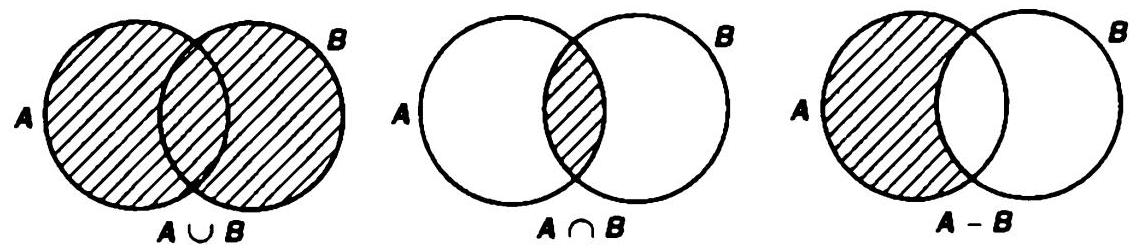
\includegraphics[width=1.0\textwidth]{images/1.1.jpg}
\end{center}
\hspace*{3em} 

Figure 1.1

\section*{Rules of Set Theory}

Given several sets, one may form new sets by applying the set-theoretic operations to them. As in algebra, one uses parentheses to indicate in what order the operations are to be performed. For example, \(A \cup  \left( {B \cap  C}\right)\) denotes the union of the two sets \(A\) and \(B \cap  C\) , while \(\left( {A \cup  B}\right)  \cap  C\) denotes the intersection of the two sets \(A \cup  B\) and \(C\) . The sets thus formed are quite different, as Figure 1.2 shows.

\begin{center}
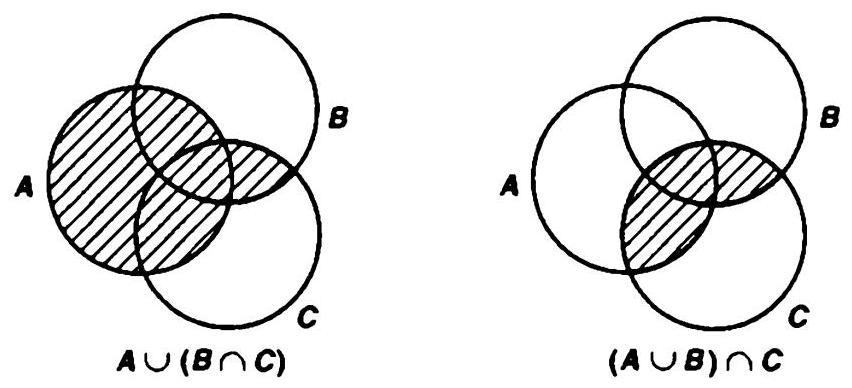
\includegraphics[width=0.7\textwidth]{images/1.2.jpg}
\end{center}
\hspace*{3em} 

Figure 1.2

Sometimes different combinations of operations lead to the same set; when that happens, one has a rule of set theory. For instance, it is true that for any sets \(A,B\) , and \(C\) the equation

\[
A \cap  \left( {B \cup  C}\right)  = \left( {A \cap  B}\right)  \cup  \left( {A \cap  C}\right)
\]

holds. The equation is illustrated in Figure 1.3; the shaded region represents the set in question, as you can check mentally. This equation can be thought of as a ``\idx{Distributive laws for  and} distributive law'' for the operations \(\cap\) and \(\cup\) .

\begin{center}
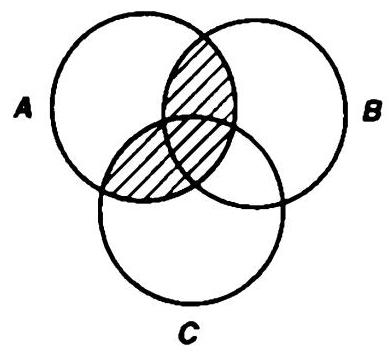
\includegraphics[width=0.3\textwidth]{images/1.3.jpg}
\end{center}
\hspace*{3em}

Figure 1.3

Other examples of set-theoretic rules include the \idx{Second coordinate of ordered pair} second ``distributive law,''

\[
A \cup  \left( {B \cap  C}\right)  = \left( {A \cup  B}\right)  \cap  \left( {A \cup  C}\right) ,
\]

and \idx{DeMorgan's laws},

\[
A - \left( {B \cup  C}\right)  = \left( {A - B}\right)  \cap  \left( {A - C}\right) ,
\]

\[
A - \left( {B \cap  C}\right)  = \left( {A - B}\right)  \cup  \left( {A - C}\right) .
\]

We leave it to you to check these rules. One can state other rules of set theory, but these are the most important ones. DeMorgan's laws are easier to remember if you verbalize them as follows:

The complement of the union equals the intersection of the complements.
The complement of the intersection equals the union of the complements.

\section*{Collections of Sets}

The objects belonging to a set may be of any sort. One can consider the set of all even integers, and the set of all blue-eyed people in Nebraska, and the set of all decks of playing cards in the world. Some of these are of limited mathematical interest, we admit! But the third example illustrates a point we have not yet mentioned: namely, that the objects belonging to a set may themselves be sets. For a deck of cards is itself a set, one consisting of pieces of pasteboard with certain standard designs printed on them. The set of all decks of cards in the world is thus a set whose elements are themselves sets (of pieces of pasteboard).

We now have another way to form new sets from old ones. Given a set \(A\) , we can consider sets whose elements are subsets of \(A\) . In particular, we can consider the set of all subsets of \(A\) . This set is sometimes denoted by the symbol \(\idxmath{P}{\(\mathcal{P}\left( A\right)\)} \mathcal{P}\left( A\right)\) and is called the \idx{power set} of \(A\) (for reasons to be explained later).

When we have a set whose elements are sets, we shall often refer to it as a \idx{collection} of sets and denote it by a script letter such as \(\mathcal{A}\) or \(\mathcal{B}\) . This device will help us in keeping things straight in arguments where we have to consider objects, and sets of objects, and collections of sets of objects, all at the same time. For example, we might use \(\mathcal{A}\) to denote the collection of all decks of cards in the world, letting an ordinary capital letter \(A\) denote a deck of cards and a lowercase letter \(a\) denote a single playing card.

A certain amount of care with notation is needed at this point. We make a distinction between the object \(a\) , which is an \idx{element of a set} \(A\) , and the one-element set \(\{ a\}\) , which is a subset of \(A\) . To illustrate, if \(A\) is the set \(\{ a,b,c\}\) , then the statements

\[
a \in  A,\;\{ a\}  \subset  A,\;\text{ and }\;\{ a\}  \in  \mathcal{P}\left( A\right)
\]

are all correct, but the statements \(\{ a\}  \in  A\) and \(a \subset  A\) are not.

\section*{Arbitrary Unions and Intersections}

We have already defined what we mean by the union and the intersection of two sets. There is no reason to limit ourselves to just two sets, for we can just as well form the union and intersection of arbitrarily many sets.

Given a collection \(\mathcal{A}\) of sets, the union of the elements of \(\mathcal{A}\) is defined by the equation

\[
\mathop{\bigcup }\limits_{{A \in  \mathcal{A}}}A = \{ x \mid  x \in  A\text{ for at least one }A \in  \mathcal{A}\} .
\]

The intersection of the elements of \(\mathcal{A}\) is defined by the equation

\[
\mathop{\bigcap }\limits_{{A \in  \mathcal{A}}}A = \{ x \mid  x \in  A\text{ for every }A \in  \mathcal{A}\} .
\]

There is no problem with these definitions if one of the elements of \(\mathcal{A}\) happens to be the empty set. But it is a bit tricky to decide what (if anything) these definitions mean if we allow \(\mathcal{A}\) to be the empty collection. Applying the definitions literally, we see that no element \(x\) satisfies the defining property for the union of the elements of \(\mathcal{A}\) . So it is reasonable to say that

\[
\mathop{\bigcup }\limits_{{A \in  A}}A = \varnothing
\]

if \(\mathcal{A}\) is empty On the other hand, every \(x\) satisfies (vacuously) the defining property for the intersection of the elements of \(\mathcal{A}\) . The question is, every \(x\) in what set? If one has a given large set \(X\) that is specified at the outset of the discussion to be one’s ``universe of discourse,'' and one considers only subsets of \(X\) throughout, it is reasonable to let

\[
\mathop{\bigcap }\limits_{{A \in  A}}A = X
\]

when \(\mathcal{A}\) is empty Not all mathematicians follow this convention, however. To avoid difficulty, we shall not define the intersection when \(\mathcal{A}\) is empty.

\section*{Cartesian Products}

There is yet another way of forming new sets from old ones; it involves the notion of an ``\idx{ordered pair}'' of objects. When you studied analytic geometry, the first thing you did was to convince yourself that after one has chosen an \(x\) -axis and a \(y\) -axis in the plane, every point in the plane can be made to correspond to a unique ordered pair(x, y)of real numbers. (In a more sophisticated treatment of geometry, the plane is more likely to be defined as the set of all ordered pairs of real numbers!)

The notion of ordered pair carries over to general sets. Given sets \(A\) and \(B\) , we define their \idx{Cartesian product: countably infinite} cartesian product \(A \times  B\) to be the set of all ordered pairs(a, b)for which \(a\) is an element of \(A\) and \(b\) is an element of \(B\) . Formally,

\[
A \times  B = \{ \left( {a,b}\right)  \mid  a \in  A\text{ and }b \in  B\} .
\]

This definition assumes that the concept of ``ordered pair'' is already given. It can be taken as a primitive concept, as was the notion of ``set''; or it can be given a definition in terms of the set operations already introduced. One definition in terms of set operations is expressed by the equation

\[
\left( {a,b}\right)  = \{ \{ a\} ,\{ a,b\} \} ;
\]

it defines the ordered pair(a, b)as a collection of sets. If \(a \neq  b\) , this definition says that (a, b)is a collection containing two sets, one of which is a one-element set and the other a two-element set. The \idx{first coordinate} of the ordered pair is defined to be the element belonging to both sets, and the second coordinate is the element belonging to only one of the sets. If \(a = b\) , then(a, b)is a collection containing only one set \(\{ a\}\) , since \(\{ a,b\}  =\)  \(\{ a,a\}  = \{ a\}\) in this case. Its first coordinate and second coordinate both equal the element in this single set.

I think it is fair to say that most mathematicians think of an ordered pair as a primitive concept rather than thinking of it as a collection of sets!

Let us make a comment on notation. It is an unfortunate fact that the notation(a, b) is firmly established in mathematics with two entirely different meanings. One meaning, as an ordered pair of objects, we have just discussed. The other meaning is the one you are familiar with from analysis; if \(a\) and \(b\) are real numbers, the symbol(a, b) is used to denote the \idx{interval} consisting of all numbers \(x\) such that \(a < x < b\) . Most of the time, this conflict in notation will cause no difficulty because the meaning will be clear from the context. Whenever a situation occurs where confusion is possible, we shall adopt a different notation for the ordered pair(a, b), denoting it by the symbol

instead.

\section*{Exercises}

1. Check the distributive laws for \(\cup\) and \(\cap\) and DeMorgan’s laws.

2. Determine which of the following statements are true for all sets \(A,B,C\) , and \(D\) . If a double implication fails, determine whether one or the other of the possible implications holds. If an equality fails, determine whether the statement becomes true if the ``equals'' symbol is replaced by one or the other of the inclusion symbols \(\subset\) or \(\supset\) .

(a) \(A \subset  B\) and \(A \subset  C \Leftrightarrow  A \subset  \left( {B \cup  C}\right)\) .

(b) \(A \subset  B\) or \(A \subset  C \Leftrightarrow  A \subset  \left( {B \cup  C}\right)\) .

(c) \(A \subset  B\) and \(A \subset  C \Leftrightarrow  A \subset  \left( {B \cap  C}\right)\) .

(d) \(A \subset  B\) or \(A \subset  C \Leftrightarrow  A \subset  \left( {B \cap  C}\right)\) .

(e) \(A - \left( {A - B}\right)  = B\) .

(f) \(A - \left( {B - A}\right)  = A - B\) .

(g) \(A \cap  \left( {B - C}\right)  = \left( {A \cap  B}\right)  - \left( {A \cap  C}\right)\) .

(h) \(A \cup  \left( {B - C}\right)  = \left( {A \cup  B}\right)  - \left( {A \cup  C}\right)\) .

(i) \(\left( {A \cap  B}\right)  \cup  \left( {A - B}\right)  = A\) .

(j) \(A \subset  C\) and \(B \subset  D \Rightarrow  \left( {A \times  B}\right)  \subset  \left( {C \times  D}\right)\) .

(k) The converse of (j).

(l) The converse of(j), assuming that \(A\) and \(B\) are nonempty.

(m) \(\left( {A \times  B}\right)  \cup  \left( {C \times  D}\right)  = \left( {A \cup  C}\right)  \times  \left( {B \cup  D}\right)\) .

(n) \(\left( {A \times  B}\right)  \cap  \left( {C \times  D}\right)  = \left( {A \cap  C}\right)  \times  \left( {B \cap  D}\right)\) .

(o) \(A \times  \left( {B - C}\right)  = \left( {A \times  B}\right)  - \left( {A \times  C}\right)\) .

(p) \(\left( {A - B}\right)  \times  \left( {C - D}\right)  = \left( {A \times  C - B \times  C}\right)  - A \times  D\) .

(q) \(\left( {A \times  B}\right)  - \left( {C \times  D}\right)  = \left( {A - C}\right)  \times  \left( {B - D}\right)\) .

3. (a) Write the contrapositive and converse of the following statement: “If \(x < 0\) , then \({x}^{2} - x > 0\) ,'' and determine which (if any) of the three statements are true.

(b) Do the same for the statement ``If \(x > 0\) , then \({x}^{2} - x > 0\) .''

4. Let \(A\) and \(B\) be sets of real numbers. Write the negation of each of the following statements:

(a) For every \(a \in  A\) , it is true that \({a}^{2} \in  B\) .

(b) For at least one \(a \in  A\) , it is true that \({a}^{2} \in  B\) .

(c) For every \(a \in  A\) , it is true that \({a}^{2} \notin  B\) .

(d) For at least one \(a \notin  A\) , it is true that \({a}^{2} \in  B\) .

5. Let \(\mathcal{A}\) be a nonempty collection of sets. Determine the truth of each of the following statements and of their converses:

(a) \(x \in  \mathop{\bigcup }\limits_{{A \in  \mathcal{A}}}A \Rightarrow  x \in  A\) for at least one \(A \in  \mathcal{A}\) .

(b) \(x \in  \mathop{\bigcup }\limits_{{A \in  \mathcal{A}}}A \Rightarrow  x \in  A\) for every \(A \in  \mathcal{A}\) .

(c) \(x \in  \mathop{\bigcap }\limits_{{A \in  \mathcal{A}}}A \Rightarrow  x \in  A\) for at least one \(A \in  \mathcal{A}\) .

(d) \(x \in  \mathop{\bigcap }\limits_{{A \in  \mathcal{A}}}A \Rightarrow  x \in  A\) for every \(A \in  \mathcal{A}\) .

6. Write the contrapositive of each of the statements of Exercise 5.

7. Given sets \(A,B\) , and \(C\) , express each of the following sets in terms of \(A,B\) , and \(C\) , using the symbols \(\cup  , \cap\) , and-.

\[
D = \{ x \mid  x \in  A\text{ and }\left( {x \in  B\text{ or }x \in  C}\right) \} ,
\]

\[
E = \{ x \mid  \left( {x \in  A\text{ and }x \in  B}\right) \text{ or }x \in  C\} ,
\]

\[
F = \{ x \mid  x \in  A\text{ and }\left( {x \in  B \Rightarrow  x \in  C}\right) \} .
\]

8. If a set \(A\) has two elements, show that \(\mathcal{P}\left( A\right)\) has four elements. How many elements does \(\mathcal{P}\left( A\right)\) have if \(A\) has one element? Three elements? No elements? Why is \(\mathcal{P}\left( A\right)\) called the power set of \(A\) ?

9. Formulate and prove DeMorgan's laws for arbitrary unions and intersections.

10. Let \(\idxmath{R}{\(\mathbb{R}\) (reals)} \mathbb{R}\) denote the set of real numbers. For each of the following subsets of \(\mathbb{R} \times  \mathbb{R}\) , determine whether it is equal to the cartesian product of two subsets of \(\mathbb{R}\) .

(a) \(\{ \left( {x,y}\right)  \mid  x\) is an integer \(\}\) .

(b) \(\{ \left( {x,y}\right)  \mid  0 < y \leq  1\}\) .

(c) \(\{ \left( {x,y}\right)  \mid  y > x\}\) .

(d) \(\{ \left( {x,y}\right)  \mid  x\) is not an integer and \(y\) is an integer \(\}\) .

(e) \(\left\{  {\left( {x,y}\right)  \mid  {x}^{2} + {y}^{2} < 1}\right\}\) .

\section*{§ 2 \idx{Function}s}

The concept of function is one you have seen many times already, so it is hardly necessary to remind you how central it is to all mathematics. In this section, we give the precise mathematical definition, and we explore some of the associated concepts.

A function is usually thought of as a rule that assigns to each element of a set \(A\) , an element of a set \(B\) . In calculus, a function is often given by a simple formula such as \(f\left( x\right)  = 3{x}^{2} + 2\) or perhaps by a more complicated formula such as

\[
f\left( x\right)  = \mathop{\sum }\limits_{{k = 1}}^{\infty }{x}^{k}
\]

One often does not even mention the sets \(A\) and \(B\) explicitly, agreeing to take \(A\) to be the set of all real numbers for which the rule makes sense and \(B\) to be the set of all real numbers.

As one goes further in mathematics, however, one needs to be more precise about what a function is. Mathematicians think of functions in the way we just described, but the definition they use is more exact. First, we define the following:

\begin{definition} A \idx{rule of assignment} is a subset \(r\) of the cartesian product \(\mathbf{C} \times  \mathbf{D}\) of two sets, having the property that each element of \(C\) appears as the first coordinate of at most one ordered pair belonging to \(r\) .


Thus, a subset \(r\) of \(C \times  D\) is a rule of assignment if

\[
\left\lbrack  {\left( {c,d}\right)  \in  r\text{ and }\left( {c,{d}^{\prime }}\right)  \in  r}\right\rbrack \Rightarrow  \left\lbrack  {d = {d}^{\prime }}\right\rbrack  .
\]

We think of \(r\) as a way of assigning, to the element \(c\) of \(C\) , the element \(d\) of \(D\) for which \(\left( {c,d}\right)  \in  r\) .

Given a rule of assignment \(r\) , the \idx{domain} of \(\mathrm{r}\) is defined to be the subset of \(C\) consisting of all first coordinates of elements of \(r\) , and the \idx{image} set of \(r\) is defined as the subset of \(D\) consisting of all second coordinates of elements of \(r\) . Formally,

\[
\text{ domain }r = \{ c \mid  \text{ there exists }d \in  D\text{ such that }\left( {c,d}\right)  \in  r\} \text{ , }
\]

\[
\text{ image }r = \{ d \mid  \text{ there exists }c \in  C\text{ such that }\left( {c,d}\right)  \in  r\} \text{ . }
\]
\end{definition}

Note that given a rule of assignment \(r\) , its domain and image are entirely determined. Now we can say what a function is.

\begin{definition} A function \(f\) is a rule of assignment \(r\) , together with a set \(B\) that contains the image set of \(r\) . The domain \(A\) of the rule \(r\) is also called the domain of the function \(f\) ; the image set of \(r\) is also called the image set of \(f\) ; and the set \(B\) is called the \idx{Range of a function} range of \(f{.}^{\dagger}\) .
\end{definition}

If \(f\) is a function having domain \(A\) and range \(B\) , we express this fact by writing

\[
f : A \rightarrow  B
\]

which is read `` \(f\) is a function from \(A\) to \(B\) ,'' or `` \(f\) is a \idx{mapping} from \(A\) into \(B\) ,'' or simply `` \(f\) maps \(A\) into \(B\) .'' One sometimes visualizes \(f\) as a geometric transformation physically carrying the points of \(A\) to points of \(B\) .

If \(f : A \rightarrow  B\) and if \(a\) is an element of \(A\) , we denote by \(f\left( a\right)\) the unique element of \(B\) that the rule determining \(f\) assigns to \(a\) ; it is called the \idx{Value of a function} value of \(f\) at \(a\) , or sometimes the image of \(a\) under \(f\) . Formally, if \(r\) is the rule of the function \(f\) , then \(f\left( a\right)\) denotes the unique element of \(B\) such that \(\left( {a,f\left( a\right) }\right)  \in  r\) .

Using this notation, one can go back to defining functions almost as one did before, with no lack of rigor. For instance, one can write (letting \(\mathbb{R}\) denote the real numbers)

``Let \(f\) be the function whose rule is \(\left\{  {\left( {x,{x}^{3} + 1}\right)  \mid  x \in  \mathbb{R}}\right\}\) and whose range is \(\mathbf{R}\) ,''

\section*{or one can equally well write}

``Let \(f : \mathbb{R} \rightarrow  \mathbb{R}\) be the function such that \(f\left( x\right)  = {x}^{3} + 1\) .''

Both sentences specify precisely the same function. But the sentence ``Let \(f\) be the function \(f\left( x\right)  = {x}^{3} + 1\) `` is no longer adequate for specifying a function because it specifies neither the domain nor the range of \(f\) .

\customfootnote{${}^{\dagger}$ Analysts are apt to use the word "range" to denote what we have called the "image set'' of \(f\). They avoid giving the set \(B\) a name.}


\begin{definition} If \(f : A \rightarrow  B\) and if \({A}_{0}\) is a subset of \(A\) , we define the restriction of \(f\) to \({A}_{0}\) to be the function mapping \({A}_{0}\) into \(B\) whose rule is

\[
\left\{  {\left( {a,f\left( a\right) }\right)  \mid  a \in  {A}_{0}}\right\}  \text{ . }
\]

It is denoted by \(f \mid  {A}_{0}\) , which is read `` \(f\) restricted to \({A}_{0}\) .''
\end{definition}


\begin{centeredblock}
\begin{example} Let \(\mathbb{R}\) denote the real numbers and let \({\bar{\mathbb{R}}}_{ + }\) denote the nonnegative reals. Consider the functions

\(f : \mathbb{R} \rightarrow  \mathbb{R}\;\) defined by \(\;f\left( x\right)  = {x}^{2},\)

\(g \cdot  {\overline{\mathbb{R}}}_{ + } \rightarrow  \mathbb{R}\;\) defined by \(\;g\left( x\right)  = {x}^{2},\)

\(h.\mathbb{R} \rightarrow  {\overline{\mathbb{R}}}_{ + }\;\) defined by \(\;h\left( x\right)  = {x}^{2}\) ,

\(k.{\overline{\mathbb{R}}}_{ + } \rightarrow  {\overline{\mathbb{R}}}_{ + }\;\) defined by \(\;k\left( x\right)  = {x}^{2}\) .

The function \(g\) is different from the function \(f\) because their rules are different subsets of \(\mathbb{R} \times  \mathbb{R}\) ; it is the restriction of \(f\) to the set \({\overline{\mathbb{R}}}_{ + }\) . The function \(h\) is also different from \(f\) , even though their rules are the same set, because the range specified for \(h\) is different from the range specified for \(f\) . The function \(k\) is different from all of these. These functions are pictured in Figure 2.1
\end{example}
\end{centeredblock}

\begin{center}
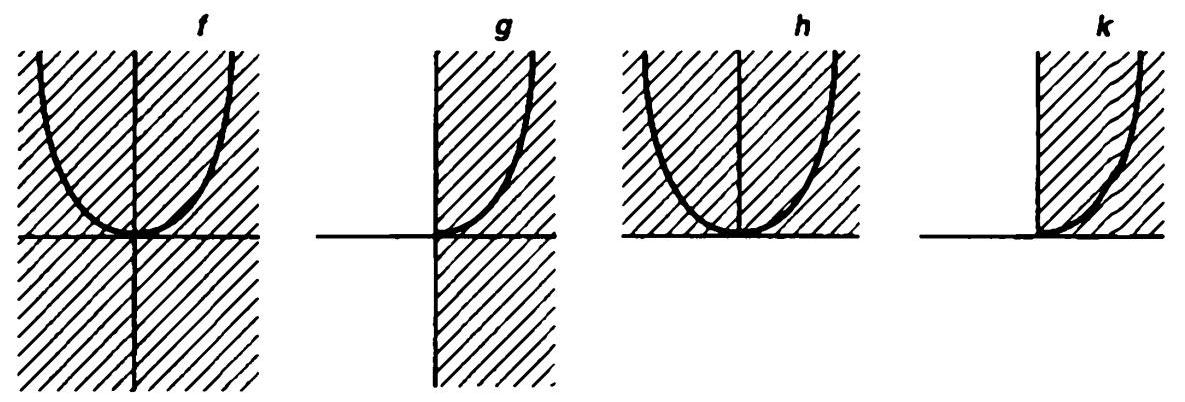
\includegraphics[width=1.0\textwidth]{images/2.1.jpg}
\end{center}
\hspace*{3em}

Figure 2.1

Restricting the domain of a function and changing its range are two ways of forming a new function from an old one. Another way is to form the \idx{Composite: of functions} composite of two functions.


\begin{definition}
    Given functions \(f : A \rightarrow  B\) and \(g : B \rightarrow  C\) , we define the composite \(g \circ  f\) of \(f\) and \(g\) as the function \(g \circ  f : A \rightarrow  C\) defined by the equation \(\left( {g \circ  f}\right) \left( a\right)  =\)  \(g\left( {f\left( a\right) }\right)\) .
\end{definition}


Formally, \(g \circ  f : A \rightarrow  C\) is the function whose rule is

\[
\{ \left( {a,c}\right)  \mid  \text{ For some }b \in  B,f\left( a\right)  = b\text{ and }g\left( b\right)  = c\} .
\]

We often picture the composite \(g \circ  f\) as involving a physical movement of the point \(a\) to the point \(f\left( a\right)\) , and then to the point \(g\left( {f\left( a\right) }\right)\) , as illustrated in Figure 2.2.

Note that \(g \circ  f\) is defined only when the range of \(f\) equals the domain of \(g\) .

\begin{center}
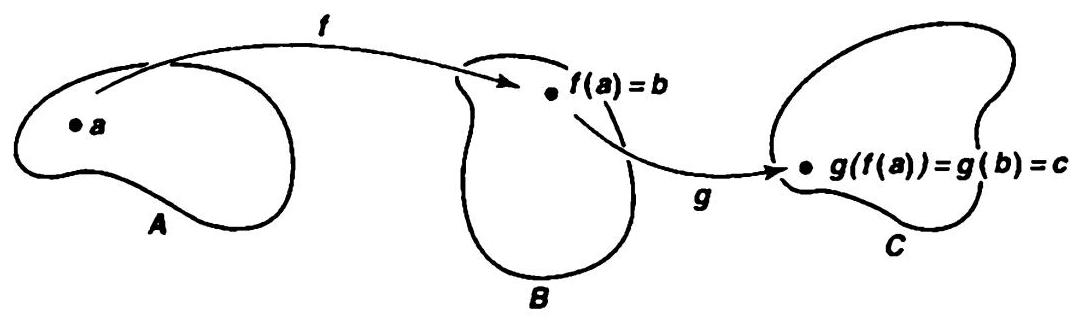
\includegraphics[width=1.0\textwidth]{images/2.2.jpg}
\end{center}
\hspace*{3em} 

Figure 2.2

\begin{example}
    The composite of the function \(f.\mathbb{R} \rightarrow  \mathbb{R}\) given by \(f\left( x\right)  = 3{x}^{2} + 2\) and the function \(g : \mathbb{R} \rightarrow  \mathbb{R}\) given by \(g\left( x\right)  = {5x}\) is the function \(g \circ  f : \mathbb{R} \rightarrow  \mathbb{R}\) given by
    \[
    \left( {g \circ  f}\right) \left( x\right)  = g\left( {f\left( x\right) }\right)  = g\left( {3{x}^{2} + 2}\right)  = 5\left( {3{x}^{2} + 2}\right) .
    \]
    The composite \(f \circ  g\) can also be formed in this case; it is the quite different function \(f \circ  g : \mathbb{R} \rightarrow  \mathbb{R}\) given by
    \[
    \left( {f \circ  g}\right) \left( x\right)  = f\left( {g\left( x\right) }\right)  = f\left( {5x}\right)  = 3{\left( 5x\right) }^{2} + 2.
    \]
\end{example}

\begin{definition}
    A function \(f : A \rightarrow  B\) is said to be injective (or one-to-one) if for each pair of distinct points of \(A\) , their images under \(f\) are distinct. It is said to be surjective (or \(f\) is said to map \(A\) onto \(B\) ) if every element of \(B\) is the image of some element of \(A\) under the function \(f\) . If \(f\) is both injective and surjective, it is said to be bijective (or is called a \idx{one-to-one correspondence}).
\end{definition}


More formally, \(f\) is injective if

\[
\left\lbrack  {f\left( a\right)  = f\left( {a}^{\prime }\right) }\right\rbrack \Rightarrow  \left\lbrack  {a = {a}^{\prime }}\right\rbrack  ,
\]

and \(f\) is surjective if

\[
\left\lbrack  {b \in  B}\right\rbrack \Rightarrow  \left\lbrack  {b = f\left( a\right) \text{ for at least one }a \in  A}\right\rbrack  .
\]

Injectivity of \(f\) depends only on the rule of \(f\) ; surjectivity depends on the range of \(f\) as well. You can check that the composite of two \idx{injective function}s is injective, and the composite of two \idx{surjective function}s is surjective; it follows that the composite of two \idx{bijective function}s is bijective.

If \(f\) is bijective, there exists a function from \(B\) to \(A\) called the \idx{Inverse function} inverse of \(f\) . It is denoted by \({f}^{-1}\) and is defined by letting \({f}^{-1}\left( b\right)\) be that unique element \(a\) of \(A\) for which \(f\left( a\right)  = b\) . Given \(b \in  B\) , the fact that \(f\) is surjective implies that there exists such an element \(a \in  A\) ; the fact that \(f\) is injective implies that there is only one such element \(a\) . It is easy to see that if \(f\) is bijective, \({f}^{-1}\) is also bijective.

\begin{example} Consider again the functions \(f,g,h\) , and \(k\) of Figure 2.1. The function \(f : \mathbb{R} \rightarrow  \mathbb{R}\) given by \(f\left( x\right)  = {x}^{2}\) is neither injective nor surjective. Its restriction \(g\) to the nonnegative reals is injective but not surjective. The function \(h : \mathbb{R} \rightarrow  \idxmath{R}{\({\mathbb{R}}_{ + }\)} {\mathbb{R}}_{ + }\) obtained from \(f\)

by changing the range is surjective but not injective. The function \(k{\overline{\mathbb{R}}}_{ + } \rightarrow  {\overline{\mathbb{R}}}_{ + }\) obtained from \(f\) by restricting the domain and changing the range is both injective and surjective, so it has an inverse. Its inverse is, of course, what we usually call the square-root function.
\end{example}

A useful criterion for showing that a given function \(f\) is bijective is the following, whose proof is left to the exercises:

\begin{lemma} Let \(f : A \rightarrow  B\) . If there are functions \(g : B \rightarrow  A\) and \(h : B \rightarrow  A\) such that \(g\left( {f\left( a\right) }\right)  = a\) for every \(a\) in \(A\) and \(f\left( {h\left( b\right) }\right)  = b\) for every \(b\) in \(B\) , then \(f\) is bijective and \(g = h = {f}^{-1}\) .
\end{lemma}

\begin{definition} Let \(f : A \rightarrow  B\) . If \({A}_{0}\) is a subset of \(A\) , we denote by \(f\left( {A}_{0}\right)\) the set of all images of points of \({A}_{0}\) under the function \(f\) ; this set is called the image of \({A}_{0}\) under \(f\) . Formally,

\[
f\left( {A}_{0}\right)  = \left\{  {b \mid  b = f\left( a\right) \text{ for at least one }a \in  {A}_{0}}\right\}  .
\]

On the other hand, if \({B}_{0}\) is a subset of \(B\) , we denote by \({f}^{-1}\left( {B}_{0}\right)\) the set of all elements of \(A\) whose images under \(f\) lie in \({B}_{0}\) ; it is called the \idx{preimage} of \({B}_{0}\) under \(f\) (or the ``\idx{counterimage},'' or the ``\idx{inverse image},'' of \({B}_{0}\) ). Formally,

\[
{f}^{-1}\left( {B}_{0}\right)  = \left\{  {a \mid  f\left( a\right)  \in  {B}_{0}}\right\}  .
\]

Of course, there may be no points \(a\) of \(A\) whose images lie in \({B}_{0}\) ; in that case, \({f}^{-1}\left( {B}_{0}\right)\) is empty.
\end{definition}

Note that if \(f : A \rightarrow  B\) is bijective and \({B}_{0} \subset  B\) , we have two meanings for the notation \({f}^{-1}\left( {B}_{0}\right)\) . It can be taken to denote the preimage of \({B}_{0}\) under the function \(f\) or to denote the image of \({B}_{0}\) under the function \({f}^{-1} : B \rightarrow  A\) . These two meanings give precisely the same subset of \(A\) , however, so there is, in fact, no ambiguity.

Some care is needed if one is to use the \(f\) and \({f}^{-1}\) notation correctly. The operation \({f}^{-1}\) , for instance, when applied to subsets of \(B\) , behaves very nicely; it preserves inclusions, unions, intersections, and differences of sets. We shall use this fact frequently. But the operation \(f\) , when applied to subsets of \(A\) , preserves only inclusions and unions. See Exercises 2 and 3.

As another situation where care is needed, we note that it is not in general true that \({f}^{-1}\left( {f\left( {A}_{0}\right) }\right)  = {A}_{0}\) and \(f\left( {{f}^{-1}\left( {B}_{0}\right) }\right)  = {B}_{0}\) . (See the following example.) The relevant rules, which we leave to you to check, are the following: If \(f : A \rightarrow  B\) and if \({A}_{0} \subset  A\) and \({B}_{0} \subset  B\) , then

\[
{A}_{0} \subset  {f}^{-1}\left( {f\left( {A}_{0}\right) }\right) \;\text{ and }\;f\left( {{f}^{-1}\left( {B}_{0}\right) }\right)  \subset  {B}_{0}.
\]

The first inclusion is an equality if \(f\) is injective, and the second inclusion is an equality if \(f\) is surjective.

\begin{example} Consider the function \(f : \mathbb{R} \rightarrow  \mathbb{R}\) given by \(f\left( x\right)  = 3{x}^{2} + 2\) (Figure 2.3) Let \(\left\lbrack  {a,b}\right\rbrack\) denote the closed interval \(a \leq  x \leq  b\) . Then

\[
{f}^{-1}\left( {f\left( \left\lbrack  {0,1}\right\rbrack  \right) }\right)  = {f}^{-1}\left( \left\lbrack  {2,5}\right\rbrack  \right)  = \left\lbrack  {-1,1}\right\rbrack  ,\;\text{ and }
\]

\[
f\left( {{f}^{-1}\left( \left\lbrack  {0,5}\right\rbrack  \right) }\right)  = f\left( \left\lbrack  {-1,1}\right\rbrack  \right)  = \left\lbrack  {2,5}\right\rbrack  .
\]
\end{example}

\begin{center}
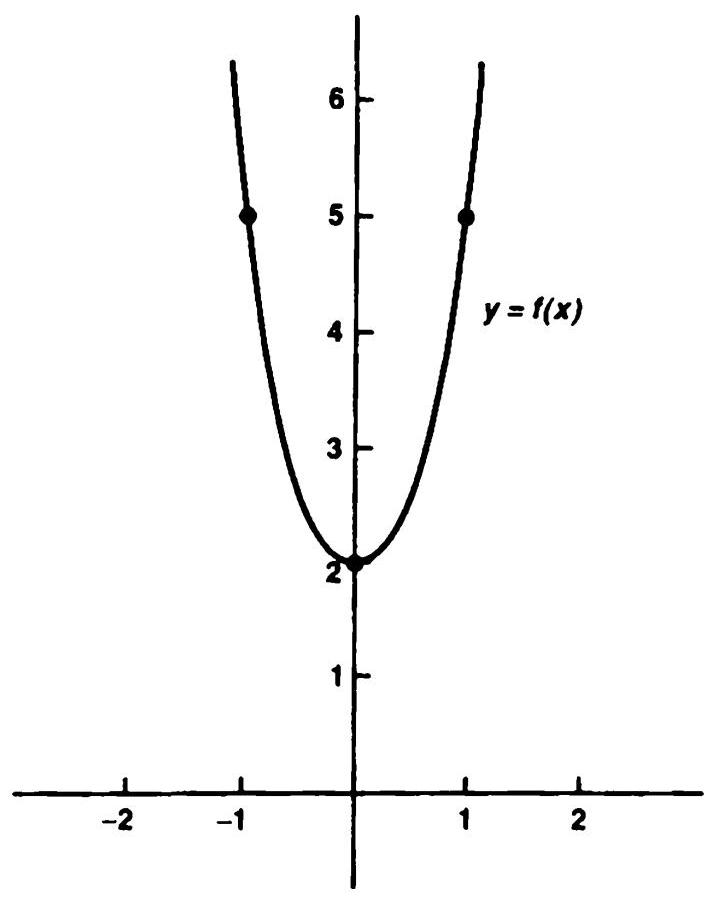
\includegraphics[width=0.6\textwidth]{images/2.3.jpg}
\end{center}
\hspace*{3em} 

Figure 2.3

\section*{Exercises}

1. Let \(f : A \rightarrow  B\) . Let \({A}_{0} \subset  A\) and \({B}_{0} \subset  B\) .

(a) Show that \({A}_{0} \subset  {f}^{-1}\left( {f\left( {A}_{0}\right) }\right)\) and that equality holds if \(f\) is injective.

(b) Show that \(f\left( {{f}^{-1}\left( {B}_{0}\right) }\right)  \subset  {B}_{0}\) and that equality holds if \(f\) is surjective.

2. Let \(f : A \rightarrow  B\) and let \({A}_{i} \subset  A\) and \({B}_{i} \subset  B\) for \(i = 0\) and \(i = 1\) . Show that \({f}^{ - }\) preserves inclusions, unions, intersections, and differences of sets:

(a) \({B}_{0} \subset  {B}_{1} \Rightarrow  {f}^{-1}\left( {B}_{0}\right)  \subset  {f}^{-1}\left( {B}_{1}\right)\) .

(b) \({f}^{-1}\left( {{B}_{0} \cup  {B}_{1}}\right)  = {f}^{-1}\left( {B}_{0}\right)  \cup  {f}^{-1}\left( {B}_{1}\right)\) .

(c) \({f}^{-1}\left( {{B}_{0} \cap  {B}_{1}}\right)  = {f}^{-1}\left( {B}_{0}\right)  \cap  {f}^{-1}\left( {B}_{1}\right)\) .

(d) \({f}^{-1}\left( {{B}_{0} - {B}_{1}}\right)  = {f}^{-1}\left( {B}_{0}\right)  - {f}^{-1}\left( {B}_{1}\right)\) .

Show that \(f\) preserves inclusions and unions only:

(e) \({A}_{0} \subset  {A}_{1} \Rightarrow  f\left( {A}_{0}\right)  \subset  f\left( {A}_{1}\right)\) .

(f) \(f\left( {{A}_{0} \cup  {A}_{1}}\right)  = f\left( {A}_{0}\right)  \cup  f\left( {A}_{1}\right)\) .

(g) \(f\left( {{A}_{0} \cap  {A}_{1}}\right)  \subset  f\left( {A}_{0}\right)  \cap  f\left( {A}_{1}\right)\) ; show that equality holds if \(f\) is injective.

(h) \(f\left( {{A}_{0} - {A}_{1}}\right)  \supset  f\left( {A}_{0}\right)  - f\left( {A}_{1}\right)\) ; show that equality holds if \(f\) is injective.

3. Show that (b), (c), (f), and (g) of Exercise 2 hold for arbitrary unions and intersections.

4. Let \(f : A \rightarrow  B\) and \(g : B \rightarrow  C\) .

(a) If \({C}_{0} \subset  C\) , show that \({\left( g \circ  f\right) }^{-1}\left( {C}_{0}\right)  = {f}^{-1}\left( {{g}^{-1}\left( {C}_{0}\right) }\right)\) .

(b) If \(f\) and \(g\) are injective, show that \(g \circ  f\) is injective.

(c) If \(g \circ  f\) is injective, what can you say about injectivity of \(f\) and \(g\) ?

(d) If \(f\) and \(g\) are surjective, show that \(g \circ  f\) is surjective.

(e) If \(g \circ  f\) is surjective, what can you say about surjectivity of \(f\) and \(g\) ?

(f) Summarize your answers to (b)-(e) in the form of a theorem.

5. In general, let us denote the \idx{identity function} for a set \(C\) by \({i}_{C}\) . That is, define \({i}_{C} : C \rightarrow  C\) to be the function given by the rule \({i}_{C}\left( x\right)  = x\) for all \(x \in  C\) . Given \(f : A \rightarrow  B\) , we say that a function \(g : B \rightarrow  A\) is a \idx{left inverse} for \(f\) if \(g \circ  f = {i}_{A}\) ; and we say that \(h : B \rightarrow  A\) is a \idx{right inverse} for \(f\) if \(f \circ  h = {i}_{B}\) .

(a) Show that if \(f\) has a left inverse, \(f\) is injective; and if \(f\) has a right inverse, \(f\) is surjective.

(b) Give an example of a function that has a left inverse but no right inverse.

(c) Give an example of a function that has a right inverse but no left inverse.

(d) Can a function have more than one left inverse? More than one right inverse?

(e) Show that if \(f\) has both a left inverse \(g\) and a right inverse \(h\) , then \(f\) is bijective and \(g = h = {f}^{-1}\) .

6. Let \(f : \mathbb{R} \rightarrow  \mathbb{R}\) be the function \(f\left( x\right)  = {x}^{3} - x\) . By restricting the domain and range of \(f\) appropriately, obtain from \(f\) a bijective function \(g\) . Draw the graphs of \(g\) and \({g}^{-1}\) . (There are several possible choices for \(g\) .)

\section*{§ 3 Relations}

A concept that is, in some ways, more general than that of function is the concept of a relation. In this section, we define what mathematicians mean by a relation, and we consider two types of relations that occur with great frequency in mathematics: \idx{equivalence relation}s and \idx{order relation}s. Order relations will be used throughout the book; equivalence relations will not be used until \(\$ {22}\) .

\begin{definition} A relation on a set \(A\) is a subset \(C\) of the cartesian product \(A \times  A\) .
\end{definition}


If \(C\) is a relation on \(A\) , we use the notation \({xCy}\) to mean the same thing as \(\left( {x,y}\right)  \in\)  \(C\) . We read it `` \(x\) is in the relation \(C\) to \(y\) .''

A rule of assignment \(r\) for a function \(f : A \rightarrow  A\) is also a subset of \(A \times  A\) . But it is a subset of a very special kind: namely, one such that each element of \(A\) appears as the first coordinate of an element of \(r\) exactly once. Any subset of \(A \times  A\) is a relation on \(A\) .

\begin{example} Let \(P\) denote the set of all people in the world, and define \(D \subset  P \times  P\) by the equation

\[
D = \{ \left( {x,y}\right)  \mid  x\text{ is a descendant of }y\} .
\]

Then \(D\) is a relation on the set \(P\) . The statements `` \(x\) is in the relation \(D\) to \(y\) `` and `` \(x\) is a descendant of \(y\) `` mean precisely the same thing, namely, that \(\left( {x,y}\right)  \in  D\) . Two other relations on \(P\) are the following

\[
B = \{ \left( {x,y}\right)  \mid  x\text{ has an ancestor who is also an ancestor of }y\} \text{ . }
\]

\[
S = \{ \left( {x,y}\right)  \mid  \text{ the parents of }x\text{ are the parents of }y\} \text{ . }
\]

We can call \(B\) the ``blood relation'' (pun intended), and we can call \(S\) the ``sibling relation.'' These three relations have quite different properties. The blood relationship is symmetric, for instance (if \(x\) is a blood relative of \(y\) , then \(y\) is a blood relative of \(x\) ), whereas the descendant relation is not. We shall consider these relations again shortly.
\end{example}

\section*{Equivalence Relations and Partitions}

An equivalence relation on a set \(A\) is a relation \(C\) on \(A\) having the following three properties:

(1) (Reflexivity) \({xCx}\) for every \(x\) in \(A\) .

(2) (Symmetry) If \({xCy}\) , then \({yCx}\) .

(3) (Transitivity) If \({xCy}\) and \({yCz}\) , then \({xCz}\) .

\begin{example} Among the relations defined in Example 1, the descendant relation \(D\) is neither reflexive nor symmetric, while the blood relation \(B\) is not transitive (I am not a blood relation to my wife, although my children are!) The sibling relation \(S\) is, however, an equivalence relation, as you may check.
\end{example}

There is no reason one must use a capital letter-or indeed a letter of any sort-to denote a relation, even though it is a set. Another symbol will do just as well. One symbol that is frequently used to denote an equivalence relation is the ``tilde'' symbol \(\sim\) . Stated in this notation, the properties of an equivalence relation become

(1) \(x \sim  x\) for every \(x\) in \(A\) .

(2) If \(x \sim  y\) , then \(y \sim  x\) .

(3) If \(x \sim  y\) and \(y \sim  z\) , then \(x \sim  z\) .

There are many other symbols that have been devised to stand for particular equivalence relations; we shall meet some of them in the pages of this book.

Given an equivalence relation \(\sim\) on a set \(A\) and an element \(x\) of \(A\) , we define a certain subset \(E\) of \(A\) , called the \idx{equivalence class} determined by \(x\) , by the equation

\[
E = \{ y \mid  y \sim  x\} .
\]

Note that the equivalence class \(E\) determined by \(x\) contains \(x\) , since \(x \sim  x\) . Equivalence classes have the following property:

\begin{lemma} Two equivalence classes \(E\) and \({E}^{\prime }\) are either disjoint or equal
\end{lemma}

\begin{proof}Let \(E\) be the equivalence class determined by \(x\) , and let \({E}^{\prime }\) be the equivalence class determined by \({x}^{\prime }\) . Suppose that \(E \cap  {E}^{\prime }\) is not empty; let \(y\) be a point of \(E \cap  {E}^{\prime }\) . See Figure 3.1. We show that \(E = {E}^{\prime }\) .
\begin{center}
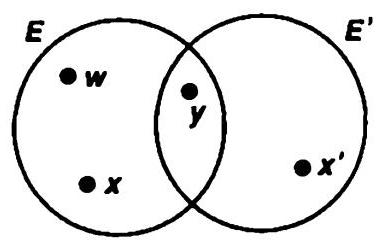
\includegraphics[width=0.3\textwidth]{images/3.1.jpg}
\end{center}
\hspace*{3em} 

Figure 3.1

By definition, we have \(y \sim  x\) and \(y \sim  {x}^{\prime }\) . Symmetry allows us to conclude that \(x \sim  y\) and \(y \sim  {x}^{\prime }\) ; from transitivity it follows that \(x \sim  {x}^{\prime }\) . If now \(w\) is any point of \(E\) , we have \(w \sim  x\) by definition; it follows from another application of transitivity that \(w \sim  {x}^{\prime }\) . We conclude that \(E \subset  {E}^{\prime }\) .

The symmetry of the situation allows us to conclude that \({E}^{\prime } \subset  E\) as well, so that \(E = {E}^{\prime }\) .

Given an equivalence relation on a set \(A\) , let us denote by \(\mathcal{E}\) the collection of all the equivalence classes determined by this relation. The preceding lemma shows that distinct elements of \(\mathcal{E}\) are disjoint. Furthermore, the union of the elements of \(\mathcal{E}\) equals all of \(A\) because every element of \(A\) belongs to an equivalence class. The collection \(\varepsilon\) is a particular example of what is called a partition of \(A\) :
\end{proof}
\begin{definition} A \idx{partition of a set} \(A\) is a collection of disjoint nonempty subsets of \(A\) whose union is all of \(A\) .
\end{definition}


Studying equivalence relations on a set \(A\) and studying partitions of \(A\) are really the same thing. Given any partition \(\mathcal{D}\) of \(A\) , there is exactly one equivalence relation on \(A\) from which it is derived.

The proof is not difficult. To show that the partition \(\mathcal{D}\) comes from some equivalence relation, let us define a relation \(C\) on \(A\) by setting \({xCy}\) if \(x\) and \(y\) belong to the same element of \(\mathcal{D}\) . Symmetry of \(C\) is obvious; reflexivity follows from the fact that the union of the elements of \(\mathcal{D}\) equals all of \(A\) ; transitivity follows from the fact that distinct elements of \(\mathcal{D}\) are disjoint It is simple to check that the collection of equivalence classes determined by \(C\) is precisely the collection \(\mathcal{D}\) .

To show there is only one such equivalence relation, suppose that \({C}_{1}\) and \({C}_{2}\) are two equivalence relations on \(A\) that give rise to the same collection of equivalence classes \(\mathcal{D}\) . Given \(x \in  A\) , we show that \(y{C}_{1}x\) if and only if \(y{C}_{2}x\) , from which we conclude that \({C}_{1} = {C}_{2}\) . Let \({E}_{1}\) be the equivalence class determined by \(x\) relative to the relation \({C}_{1}\) ; let \({E}_{2}\) be the equivalence class determined by \(x\) relative to the relation \({C}_{2}\) . Then \({E}_{1}\) is an element of \(\mathcal{D}\) , so that it must equal the unique element \(D\) of \(\mathcal{D}\) that contains \(x\) . Similarly, \({E}_{2}\) must equal \(D\) . Now by definition, \({E}_{1}\) consists of all \(y\) such that \(y{C}_{1}x\) ; and \({E}_{2}\) consists of all \(y\) such that \(y{C}_{2}x\) . Since \({E}_{1} = D = {E}_{2}\) , our result is proved.

\begin{example} Define two points in the plane to be equivalent if they lie at the same distance from the ongin. Reflexivity, symmetry, and transitivity hold trivially. The collection \(\varepsilon\) of equivalence classes consists of all circles centered at the origin, along with the set consisting of the origin alone.
\end{example}

\begin{example} Define two points of the plane to be equivalent if they have the same \(y\) -coordinate. The collection of equivalence classes is the collection of all straight lines in the plane parallel to the \(x\) -axis.
\end{example}

\begin{example} Let \(\mathcal{L}\) be the collection of all straight lines in the plane parallel to the line \(y =  - x\) . Then \(\mathcal{L}\) is a partition of the plane, since each point lies on exactly one such line. The partition \(\mathcal{L}\) comes from the equivalence relation on the plane that declares the points \(\left( {{x}_{0},{y}_{0}}\right)\) and \(\left( {{x}_{1},{y}_{1}}\right)\) to be equivalent if \({x}_{0} + {y}_{0} = {x}_{1} + {y}_{1}\) .
\end{example}

\begin{example} Let \({\mathcal{L}}^{\prime }\) be the collection of all straight lines in the plane. Then \({\mathcal{L}}^{\prime }\) is not a partition of the plane, for distinct elements of \({\mathcal{L}}^{\prime }\) are not necessarily disjoint; two lines may intersect without being equal.
\end{example}

\section*{Order Relations}

A relation \(C\) on a set \(A\) is called an order relation (or a \idx{simple order}, or a \idx{linear order}) if it has the following properties:

(1) (\idx{Comparability: of cardinalities} Comparability) For every \(x\) and \(y\) in \(A\) for which \(x \neq  y\) , either \({xCy}\) or \({yCx}\) .

(2) (Nonreflexivity) For no \(x\) in \(A\) does the relation \({xCx}\) hold.

(3) (Transitivity) If \({xCy}\) and \({yCz}\) , then \({xCz}\) .

Note that property (1) does not by itself exclude the possibility that for some pair of elements \(x\) and \(y\) of \(A\) , both the relations \({xCy}\) and \({yCx}\) hold (since ``or'' means ``one or the other, or both''). But properties (2) and (3) combined do exclude this possibility; for if both \({xCy}\) and \({yCx}\) held, transitivity would imply that \({xCx}\) , contradicting nonreflexivity.

\begin{example} Consider the relation on the real line consisting of all pairs(x, y)of real numbers such that \(x < y\) . It is an order relation, called the ``usual order relation,'' on the real line. A less familiar order relation on the real line is the following: Define \({xCy}\) if \({x}^{2} < {y}^{2}\) , or if \({x}^{2} = {y}^{2}\) and \(x < y\) . You can check that this is an order relation.
\end{example}

\begin{example} Consider again the relationships among people given in Example 1. The blood relation \(B\) satisfies none of the properties of an order relation, and the sibling relation \(S\) satisfies only (3). The descendant relation \(D\) does somewhat better, for it satisfies both (2) and (3); however, comparability still fails. Relations that satisfy (2) and (3) occur often enough in mathematics to be given a special name. They are called strict \idx{partial order} relations; we shall consider them later (see \(§{11}\) ).
\end{example}

As the tilde, \(\sim\) , is the generic symbol for an equivalence relation, the ``less than'' symbol, \(<\) , is commonly used to denote an order relation. Stated in this notation, the properties of an order relation become

(1) If \(x \neq  y\) , then either \(x < y\) or \(y < x\) .

(2) If \(x < y\) , then \(x \neq  y\) .

(3) If \(x < y\) and \(y < z\) , then \(x < z\) .

We shall use the notation \(x \leq  y\) to stand for the statement ``either \(x < y\) or \(x = y\) ``; and we shall use the notation \(y > x\) to stand for the statement `` \(x < y\) .'' We write \(x < y < z\) to mean `` \(x < y\) and \(y < z\) .''

\begin{definition} If \(X\) is a set and \(<\) is an order relation on \(X\) , and if \(a < b\) , we use the notation(a, b)to denote the set

\[
\{ x \mid  a < x < b\} \text{ ; }
\]

it is called an \idx{open interval} in \(X\) . If this set is empty, we call a the \idx{immediate predecessor} of \(b\) , and we call \(b\) the \idx{immediate successor} of \(a\) .
\end{definition}


\begin{definition} Suppose that \(A\) and \(B\) are two sets with order relations \({ < }_{A}\) and \({ < }_{B}\) respectively. We say that \(A\) and \(B\) have the same \idx{order type} if there is a bijective correspondence between them that preserves order; that is, if there exists a bijective function \(f : A \rightarrow  B\) such that

\[
{a}_{1}{ < }_{A}{a}_{2} \Rightarrow  f\left( {a}_{1}\right) { < }_{B}f\left( {a}_{2}\right) .
\]
\end{definition}


\begin{example} The interval(-1,1)of real numbers has the same order type as the set \(\mathbb{R}\) of real numbers itself, for the function \(f : \left( {-1,1}\right)  \rightarrow  \mathbb{R}\) given by

\[
f\left( x\right)  = \frac{x}{1 - {x}^{2}}
\]

is an order-preserving bijective correspondence, as you can check. It is pictured in Figure 3.2.
\end{example}

\begin{example} The subset \(A = \{ 0\}  \cup  \left( {1,2}\right)\) of \(\mathbb{R}\) has the same order type as the subset

\[
\lbrack 0,1) = \{ x \mid  0 \leq  x < 1\}
\]

of \(\mathbb{R}\) . The function \(f : A \rightarrow  \lbrack 0,1)\) defined by

\[
f\left( 0\right)  = 0,
\]

\[
f\left( x\right)  = x - 1\;\text{ for }x \in  \left( {1,2}\right)
\]

is the required order-preserving correspondence.
\end{example}

One interesting way of defining an order relation, which will be useful to us later in dealing with some examples, is the following:

\begin{center}
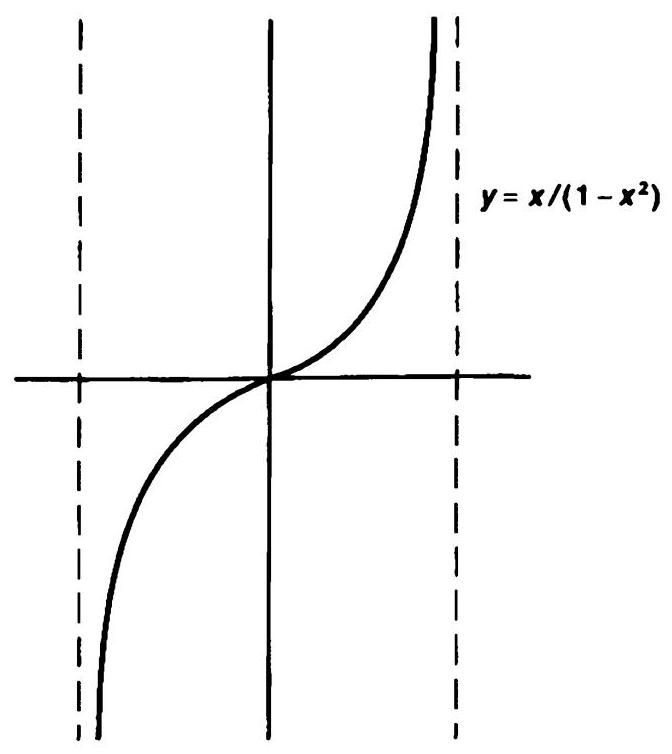
\includegraphics[width=0.6\textwidth]{images/3.2.jpg}
\end{center}
\hspace*{3em} 

Figure 3.2

\begin{definition} Suppose that \(A\) and \(B\) are two sets with order relations \({ < }_{A}\) and \({ < }_{B}\) respectively. Define an order relation \(<\) on \(A \times  B\) by defining

\[
{a}_{1} \times  {b}_{1} < {a}_{2} \times  {b}_{2}
\]

if \({a}_{1}{ < }_{A}{a}_{2}\) , or if \({a}_{1} = {a}_{2}\) and \({b}_{1}{ < }_{B}{b}_{2}\) . It is called the \idx{dictionary order} relation on \(A \times  B\) .
\end{definition}

Checking that this is an order relation involves looking at several separate cases; we leave it to you.

The reason for the choice of terminology is fairly evident. The rule defining \(<\) is the same as the rule used to order the words in the dictionary. Given two words, one compares their first letters and orders the words according to the order in which their first letters appear in the alphabet. If the first letters are the same, one compares their second letters and orders accordingly. And so on.


\begin{example} Consider the dictionary order on the plane \(\mathbb{R} \times  \mathbb{R}\) . In this order, the point \(p\) is less than every point lying above it on the vertical line through \(p\) , and \(p\) is less than every point to the right of this vertical line.
\end{example}

\begin{example} Consider the set \(\lbrack 0,1)\) of real numbers and the set \(\idxmath{Z}{\({\mathbb{Z}}_{ + }\)} {\idxmath{Z}{\(\mathbb{Z}\)} \mathbb{Z}}_{ + }\) of \idx{positive integers}, both in their usual orders; give \({\mathbb{Z}}_{ + } \times  \lbrack 0,1)\) the dictionary order. This set has the same order type as the set of nonnegative reals; the function

\[
f\left( {n \times  t}\right)  = n + t - 1
\]

is the required bijective order-preserving correspondence. On the other hand, the set \(\left( {0,1}\right)  \times  {\mathbb{Z}}_{ + }\) in the dictionary order has quite a different order type; for example, every element of this ordered set has an immediate successor. These sets are pictured in Figure 3.3.
\end{example}

\begin{center}
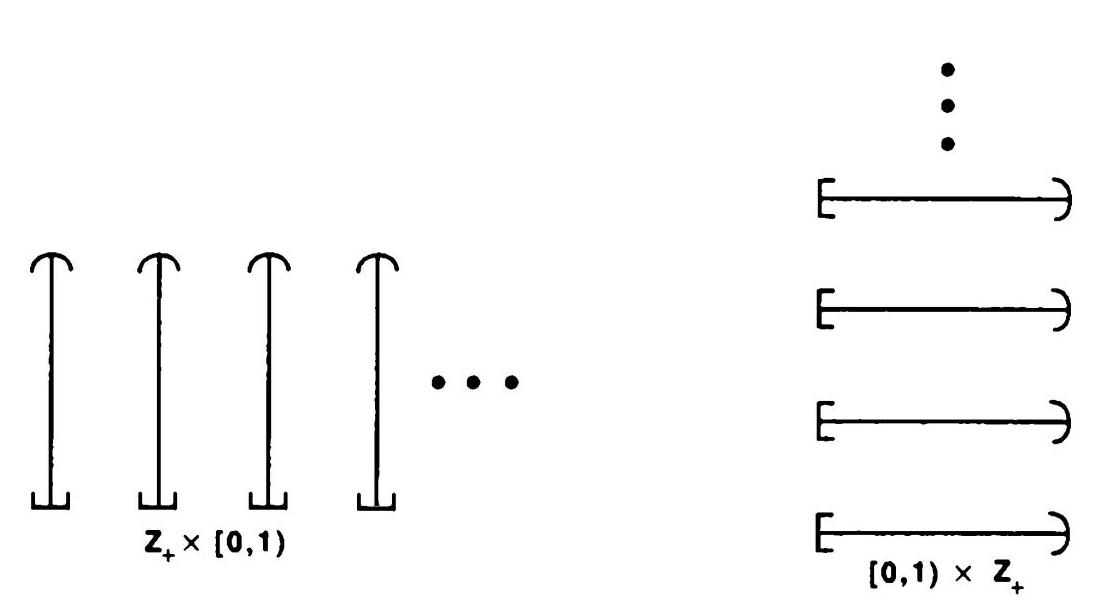
\includegraphics[width=1.0\textwidth]{images/3.3.jpg}
\end{center}
\hspace*{3em}

Figure 3.3

One of the properties of the real numbers that you may have seen before is the “least \idx{upper bound} property.” One can define this property for an arbitrary ordered set. First, we need some preliminary definitions.

Suppose that \(A\) is a set ordered by the relation \(<\) . Let \({A}_{0}\) be a subset of \(A\) . We say that the element \(b\) is the \idx{largest element} of \({A}_{0}\) if \(b \in  {A}_{0}\) and if \(x \leq  b\) for every \(x \in  {A}_{0}\) . Similarly, we say that \(a\) is the \idx{Smallest element of ordered set} smallest element of \({A}_{0}\) if \(a \in  {A}_{0}\) and if \(a \leq  x\) for every \(x \in  {A}_{0}\) . It is easy to see that a set has at most one largest element and at most one smallest element.

We say that the subset \({A}_{0}\) of \(A\) is \idx{bounded above} if there is an element \(b\) of \(A\) such that \(x \leq  b\) for every \(x \in  {A}_{0}\) ; the element \(b\) is called an upper bound for \({A}_{0}\) . If the set of all upper bounds for \({A}_{0}\) has a smallest element, that element is called the least upper bound, or the \idx{supremum}, of \({A}_{0}\) . It is denoted by sup \({A}_{0}\) ; it may or may not belong to \({A}_{0}\) . If it does, it is the largest element of \({A}_{0}\) .

Similarly, \({A}_{0}\) is \idx{bounded below} if there is an element \(a\) of \(A\) such that \(a \leq  x\) for every \(x \in  {A}_{0}\) ; the element \(a\) is called a \idx{lower bound} for \({A}_{0}\) . If the set of all lower bounds for \({A}_{0}\) has a largest element, that element is called the \idx{greatest lower bound}, or the \idx{infimum}, of \({A}_{0}\) . It is denoted by inf \({A}_{0}\) , it may or may not belong to \({A}_{0}\) . If it does, it is the smallest element of \({A}_{0}\) .

Now we can define the least upper bound property.

\begin{definition} An ordered set \(A\) is said to have the least upper bound property if every nonempty subset \({A}_{0}\) of \(A\) that is bounded above has a least upper bound. Analogously, the set \(A\) is said to have the greatest lower bound property if every nonempty subset \({A}_{0}\) of \(A\) that is bounded below has a greatest lower bound.
\end{definition}


We leave it to the exercises to show that \(A\) has the least upper bound property if and only if it has the greatest lower bound property.

\begin{example} Consider the set \(A = \left( {-1,1}\right)\) of real numbers in the usual order. Assuming the fact that the real numbers have the least upper bound property, it follows that the set \(A\) has the least upper bound property. For, given any subset of \(A\) having an upper bound in \(A\) , it follows that its least upper bound (in the real numbers) must be in \(A\) . For example, the subset \(\left\{  {-1/{2n} \mid  n \in  {\mathbb{Z}}_{ + }}\right\}\) of \(A\) , though it has no largest element, does have a least upper bound in \(A\) , the number 0 .

On the other hand, the set \(B = \left( {-1,0}\right)  \cup  \left( {0,1}\right)\) does not have the least upper bound property. The subset \(\left\{  {-1/{2n} \mid  n \in  {\mathbb{Z}}_{ + }}\right\}\) of \(B\) is bounded above by any element of(0,1), but it has no least upper bound in \(B\) .
\end{example}

\section*{Exercises}

Equivalence Relations

1. Define two points \(\left( {{x}_{0},{y}_{0}}\right)\) and \(\left( {{x}_{1},{y}_{1}}\right)\) of the plane to be equivalent if \({y}_{0} - {x}_{0}^{2} =\)  \({y}_{1} - {x}_{1}^{2}\) . Check that this is an equivalence relation and describe the equivalence classes

2. Let \(C\) be a relation on a set \(A\) . If \({A}_{0} \subset  A\) , define the restriction of \(C\) to \({A}_{0}\) to be the relation \(C \cap  \left( {{A}_{0} \times  {A}_{0}}\right)\) . Show that the restriction of an equivalence relation is an equivalence relation.

3. Here is a ``proof'' that every relation \(C\) that is both symmetric and transitive is also reflexive: ``Since \(C\) is symmetric, \({aCb}\) implies \({bCa}\) . Since \(C\) is transitive, \({aCb}\) and \({bCa}\) together imply \({aCa}\) , as desired.'' Find the flaw in this argument.

4. Let \(f : A \rightarrow  B\) be a surjective function. Let us define a relation on \(A\) by setting \({a}_{0} \sim  {a}_{1}\) if

\[
f\left( {a}_{0}\right)  = f\left( {a}_{1}\right) .
\]

(a) Show that this is an equivalence relation.

(b) Let \({A}^{ * }\) be the set of equivalence classes. Show there is a bijective correspondence of \({A}^{ * }\) with \(B\) .

5. Let \(S\) and \({S}^{\prime }\) be the following subsets of the plane.

\[
S = \{ \left( {x,y}\right)  \mid  y = x + 1\text{ and }0 < x < 2\} ,
\]

\[
{S}^{\prime } = \{ \left( {x,y}\right)  \mid  y - x\text{ is an integer }\} .
\]

(a) Show that \({S}^{\prime }\) is an equivalence relation on the real line and \({S}^{\prime } \supset  S\) . Describe the equivalence classes of \({S}^{\prime }\) .

(b) Show that given any collection of equivalence relations on a set \(A\) , their intersection is an equivalence relation on \(A\) .

(c) Describe the equivalence relation \(T\) on the real line that is the intersection of all equivalence relations on the real line that contain \(S\) . Describe the equivalence classes of \(T\) .

\section*{Order Relations}

6. Define a relation on the plane by setting

\[
\left( {{x}_{0},{y}_{0}}\right)  < \left( {{x}_{1},{y}_{1}}\right)
\]

if either \({y}_{0} - {x}_{0}^{2} < {y}_{1} - {x}_{1}^{2}\) , or \({y}_{0} - {x}_{0}^{2} = {y}_{1} - {x}_{1}^{2}\) and \({x}_{0} < {x}_{1}\) . Show that this is an order relation on the plane, and describe it geometrically.

7. Show that the restriction of an order relation is an order relation.

8. Check that the relation defined in Example 7 is an order relation.

9. Check that the dictionary order is an order relation.

10. (a) Show that the map \(f : \left( {-1,1}\right)  \rightarrow  \mathbb{R}\) of Example 9 is order preserving.

(b) Show that the equation \(g\left( y\right)  = {2y}/\left\lbrack  {1 + {\left( 1 + 4{y}^{2}\right) }^{1/2}}\right\rbrack\) defines a function \(g : \mathbb{R} \rightarrow  \left( {-1,1}\right)\) that is both a left and a right inverse for \(f\) .

11. Show that an element in an ordered set has at most one immediate successor and at most one immediate predecessor. Show that a subset of an ordered set has at most one smallest element and at most one largest element.

12. Let \({\mathbb{Z}}_{ + }\) denote the set of positive integers. Consider the following order relations on \({\mathbb{Z}}_{ + } \times  {\mathbb{Z}}_{ + }\) :

(i) The dictionary order.

(ii) \(\left( {{x}_{0},{y}_{0}}\right)  < \left( {{x}_{1},{y}_{1}}\right)\) if either \({x}_{0} - {y}_{0} < {x}_{1} - {y}_{1}\) , or \({x}_{0} - {y}_{0} = {x}_{1} - {y}_{1}\) and \({y}_{0} < {y}_{1}\) .

(iii) \(\left( {{x}_{0},{y}_{0}}\right)  < \left( {{x}_{1},{y}_{1}}\right)\) if either \({x}_{0} + {y}_{0} < {x}_{1} + {y}_{1}\) , or \({x}_{0} + {y}_{0} = {x}_{1} + {y}_{1}\) and \({y}_{0} < {y}_{1}\) .

In these order relations, which elements have immediate predecessors? Does the set have a smallest element? Show that all three order types are different.

13. Prove the following:

\begin{theorem} 
    If an ordered set \(A\) has the least upper bound property, then it has the greatest lower bound property.
\end{theorem}

14. If \(C\) is a relation on a set \(A\) , define a new relation \(D\) on \(A\) by letting \(\left( {b,a}\right)  \in  D\) if \(\left( {a,b}\right)  \in  C\) .

(a) Show that \(C\) is symmetric if and only if \(C = D\) .

(b) Show that if \(C\) is an order relation, \(D\) is also an order relation.

(c) Prove the converse of the theorem in Exercise 13.

15. Assume that the real line has the least upper bound property.

(a) Show that the sets

\[
\left\lbrack  {0,1}\right\rbrack = \{ x \mid  0 \leq  x \leq  1\} ,
\]

\[
\lbrack 0,1) = \{ x \mid  0 \leq  x < 1\rbrack
\]

have the least upper bound property.

(b) Does \(\left\lbrack  {0,1}\right\rbrack \times  \left\lbrack  {0,1}\right\rbrack\) in the dictionary order have the least upper bound property? What about \(\left\lbrack  {0,1}\right\rbrack \times  \lbrack 0,1)\) ? What about \(\lbrack 0,1) \times  \left\lbrack  {0,1}\right\rbrack\) ?

\section*{§ 4 The Integers and the Real Numbers}

Up to now we have been discussing what might be called the logical foundations for our study of topology-the elementary concepts of set theory. Now we turn to what we might call the mathematical foundations for our study-the integers and the real number system. We have already used them in an informal way in the examples and exercises of the preceding sections. Now we wish to deal with them more formally.

One way of establishing these foundations is to construct the real number system, using only the axioms of set theory-to build them with one's bare hands, so to speak. This way of approaching the subject takes a good deal of time and effort and is of greater logical than mathematical interest.

A second way is simply to assume a set of axioms for the real numbers and work from these axioms. In the present section, we shall sketch this approach to the real numbers. Specifically, we shall give a set of axioms for the real numbers and shall indicate how the familiar properties of real numbers and the integers are derived from them. But we shall leave most of the proofs to the exercises. If you have seen all this before, our description should refresh your memory. If not, you may want to work through the exercises in detail in order to make sure of your knowledge of the mathematical foundations.

First we need a definition from set theory.

\section*{Definition. A binary operation on a set \(A\) is a function \(f\) mapping \(A \times  A\) into \(A\) .}

When dealing with a \idx{binary operation} \(f\) on a set \(A\) , we usually use a notation different from the standard functional notation introduced in \(\$ 2\) . Instead of denoting the value of the function \(f\) at the point \(\left( {a,{a}^{\prime }}\right)\) by \(f\left( {a,{a}^{\prime }}\right)\) , we usually write the symbol for the function between the two coordinates of the point in question, writing the value of the function at \(\left( {a,{a}^{\prime }}\right)\) as \({af}{a}^{\prime }\) . Furthermore (just as was the case with relations), it is more common to use some symbol other than a letter to denote an operation. Symbols often used are the plus symbol +, the multiplication symbols - and -, and the asterisk \(*\) ; however, there are many others.

\section*{Assumption}

We assume there exists a set \(\mathbb{R}\) , called the set of real numbers, two binary operations + and \(\cdot\) on \(\mathbb{R}\) , called the addition and multiplication operations, respectively, and an order relation \(<\) on \(\mathbb{R}\) , such that the following properties hold:

Algebraic Properties

(l) \(\left( {x + y}\right)  + z = x + \left( {y + z}\right)\) ,

\(\left( {x \cdot  y}\right)  \cdot  z = x \cdot  \left( {y \cdot  z}\right)\) for all \(x,y,z\) in \(\mathbb{R}\) .

(2) \(x + y = y + x\) .

\(x \cdot  y = y \cdot  x\) for all \(x,y\) in \(\mathbb{R}\) .

(3) There exists a unique element of \(\mathbb{R}\) called zero, denoted by 0, such that \(x + 0 = x\) for all \(x \in  \mathbb{R}\) .

There exists a unique element of \(\mathbb{R}\) called one, different from 0 and denoted by 1, such that \(x \cdot  1 = x\) for all \(x \in  \mathbb{R}\) .

(4) For each \(x\) in \(\mathbb{R}\) , there exists a unique \(y\) in \(\mathbb{R}\) such that \(x + y = 0\) .

For each \(x\) in \(\mathbb{R}\) different from 0, there exists a unique \(y\) in \(\mathbb{R}\) such that \(x \cdot  y = 1\) .

(5) \(x \cdot  \left( {y + z}\right)  = \left( {x \cdot  y}\right)  + \left( {x \cdot  z}\right)\) for all \(x,y,z \in  \mathbb{R}\) .

A Mixed Algebraic and Order Property

(6) If \(x > y\) , then \(x + z > y + z\) .

If \(x > y\) and \(z > 0\) , then \(x \cdot  z > y \cdot  z\) .

\section*{Order Properties}

(7) The order relation \(<\) has the least upper bound property.

(8) If \(x < y\) , there exists an element \(z\) such that \(x < z\) and \(z < y\) .

From properties (1)-(5) follow the familiar ``laws of algebra.'' Given \(x\) , one denotes by \(- x\) that number \(y\) such that \(x + y = 0\) ; it is called the negative of \(x\) . One defines the subtraction operation by the formula \(z - x = z + \left( {-x}\right)\) . Similarly, given \(x \neq  0\) , one denotes by \(1/x\) that number \(y\) such that \(x \cdot  y = 1\) ; it is called the reciprocal of \(x\) . One defines the quotient \(z/x\) by the formula \(z/x = z \cdot  \left( {1/x}\right)\) . The usual laws of signs, and the rules for adding and multiplying fractions, follow as theorems. These laws of algebra are listed in Exercise 1 at the end of the section. We often denote \(xy\)  \(\operatorname{simplyby}{xy}\) .

When one adjoins property (6) to properties (I)-(5), one can prove the usual ``laws of inequalities,'' such as the following:

\[
\text{ If }x > y\text{ and }z < 0\text{ , then }x \cdot  z < y \cdot  z\text{ . }
\]

\[
- 1 < 0\text{ and }0 < 1\text{ . }
\]

The laws of inequalities are listed in Exercise 2.

We define a number \(x\) to be positive if \(x > 0\) , and to be negative if \(x < 0\) . We denote the positive reals by \({\mathbb{R}}_{ + }\) and the nonnegative reals (for reasons to be explained later) by \({\overline{\mathbb{R}}}_{ + }\) . Properties (1)-(6) are familiar properties in modern algebra. Any set with two binary operations satisfying (1)-(5) is called by algebraists afield; if the field has an order relation satisfying (6), it is called an \idx{ordered field}.

Properties (7) and (8), on the other hand, are familiar properties in topology. They involve only the order relation; any set with an order relation satisfying (7) and (8) is called by topologists a \idx{linear continuum}.

Now it happens that when one adjoins to the axioms for an ordered field [properties (l)-(6)] the axioms for a linear continuum [properties (7) and (8)], the resulting list contains some redundancies. Property (8), in particular, can be proved as a consequence of the others; given \(x < y\) one can show that \(z = \left( {x + y}\right) /\left( {1 + 1}\right)\) satisfies the requirements of (8). Therefore, in the standard treatment of the real numbers, properties (1)-(7) are taken as axioms, and property (8) becomes a theorem. We have included (8) in our list merely to emphasize the fact that it and the least upper bound property are the two crucial properties of the order relation for \(\mathbb{R}\) . From these two properties many of the topological properties of \(\mathbb{R}\) may be derived, as we shall see in Chapter 3.

Now there is nothing in this list as it stands to tell us what an integer is. We now define the integers, using only properties (1)-(6).

\begin{definition} A subset \(A\) of the real numbers is said to be inductive if it contains the number 1, and if for every \(x\) in \(A\) , the number \(x + 1\) is also in \(A\) . Let \(\mathcal{A}\) be the collection of all inductive subsets of \(\mathbb{R}\) . Then the set \({\mathbb{Z}}_{ + }\) of positive integers is defined by the equation


\[
{\mathbb{Z}}_{ + } = \mathop{\bigcap }\limits_{{A \in  A}}A
\]
\end{definition}

Note that the set \({\mathbb{R}}_{ + }\) of positive real numbers is inductive, for it contains 1 and the statement \(x > 0\) implies the statement \(x + 1 > 0\) . Therefore, \({\mathbb{Z}}_{ + } \subset  {\mathbb{R}}_{ + }\) , so the elements of \({\mathbb{Z}}_{ + }\) are indeed positive, as the choice of terminology suggests. Indeed, one sees readily that1is the smallest element of \({\mathbb{Z}}_{ + }\) , because the set of all real numbers \(x\) for which \(x \geq  1\) is inductive.

The basic properties of \({\mathbb{Z}}_{ + }\) , which follow readily from the definition, are the following:

(I) \({\mathbb{Z}}_{ + }\) is inductive.

(2) (\idx{Principle of induction}). If \(A\) is an \idx{inductive set} of positive integers, then \(A =\)  \({Z}_{ + }\) .

We define the set \(\mathbb{Z}\) of integers to be the set consisting of the positive integers \({\mathbb{Z}}_{ + }\) , the number 0, and the negatives of the elements of \({\mathbb{Z}}_{ + }\) . One proves that the sum, difference, and product of two integers are integers, but the quotient is not necessarily an integer. The set \(\mathbb{Q}\) of quotients of integers is called the set of \idx{rational number}s.

One proves also that, given the integer \(n\) , there is no integer \(a\) such that \(n < a <\)  \(n + 1\) .

If \(n\) is a positive integer, we use the symbol \({S}_{n}\) to denote the set of all positive integers less than \(n\) ; we call it a section of the positive integers. The set \({S}_{1}\) is empty, and \({S}_{n + 1}\) denotes the set of positive integers between1and \(n\) , inclusive. We also use the notation

\[
\{ 1,\ldots ,n\}  = {S}_{n + 1}
\]

for the latter set.

Now we prove two properties of the positive integers that may not be quite so familiar, but are quite useful. They may be thought of as alternative versions of the \idx{induction principle}.

\begin{theorem}[Well-ordering property] Every nonempty subset of \({\mathbb{Z}}_{ + }\) has a smallest element.
\end{theorem}
\begin{proof} We first prove that, for each \(n \in  {\mathbb{Z}}_{ + }\) , the following statement holds: Every nonempty subset of \(\{ 1,\ldots ,n\}\) has a smallest element.

Let \(A\) be the set of all positive integers \(\mathrm{n}\) for which this statement holds. Then \(A\) contains 1, since if \(n = 1\) , the only nonempty subset of \(\{ 1,\ldots ,n\}\) is the set \(\{ 1\}\) itself. Then, supposing \(A\) contains \(n\) , we show that it contains \(n + 1\) . So let \(C\) be a nonempty subset of the set \(\{ 1,\ldots ,n + 1\}\) . If \(C\) consists of the single element \(n + 1\) , then that element is the smallest element of \(C\) . Otherwise, consider the set \(C \cap  \{ 1,\ldots ,n\}\) , which is nonempty. Because \(n \in  A\) , this set has a smallest element, which will automatically be the smallest element of \(C\) also. Thus \(A\) is inductive, so we conclude that \(A = {\mathbb{Z}}_{ + }\) ; hence the statement is true for all \(n \in  {\mathbb{Z}}_{ + }\) .

Now we prove the theorem. Suppose that \(D\) is a nonempty subset of \({\mathbb{Z}}_{ + }\) . Choose an element \(n\) of \(D\) . Then the set \(A = D \cap  \{ 1,\ldots ,n\}\) is nonempty, so that \(A\) has a smallest element \(k\) . The element \(k\) is automatically the smallest element of \(D\) as well.
\end{proof}

\begin{theorem}[\idx{Strong induction principle}] Let \(A\) be a set of positive integers. Suppose that for each posiave integer \(n\) , the statement \({S}_{n} \subset  A\) implies the statement \(n \in  A\) . Then \(A = {\mathbb{Z}}_{ + }\) .
\end{theorem}

\begin{proof}If \(A\) does not equal all of \({\mathbb{Z}}_{ + }\) , let \(n\) be the smallest positive integer that is not in \(A\) . Then every positive integer less than \(n\) is in \(A\) , so that \({S}_{n} \subset  A\) . Our hypothesis implies that \(n \in  A\) , contrary to assumption.
Everything we have done up to now has used only the axioms for an ordered field, properties (1)-(6) of the real numbers. At what point do you need (7), the least upper bound axiom?

For one thing, you need the least upper bound axiom to prove that the set \({\mathbb{Z}}_{ + }\) of positive integers has no upper bound in \(\mathbb{R}\) . This is the \idx{Archimedean ordering} property of the real line. To prove it, we assume that \({\mathbb{Z}}_{ + }\) has an upper bound and derive a contradiction. If \({\mathbb{Z}}_{ + }\) has an upper bound, it has a least upper bound \(b\) . There exists \(n \in  {\mathbb{Z}}_{ + }\) such that \(n > b - 1\) ; for otherwise, \(b - 1\) would be an upper bound for \({\mathbb{Z}}_{ + }\) smaller than \(b\) . Then \(n + 1 > b\) , contrary to the fact that \(b\) is an upper bound for \({\mathbb{Z}}_{ + }\) .

The least upper bound axiom is also used to prove a number of other things about \(\mathbb{R}\) . It is used for instance to show that \(\mathbb{R}\) has the greatest lower bound property. It is also used to prove the existence of a unique positive square root \(\sqrt{x}\) for every positive real number. This fact, in turn, can be used to demonstrate the existence of real numbers that are not rational numbers; the number \(\sqrt{2}\) is an easy example.

We use the symbol 2 to denote \(l + l\) , the symbol 3 to denote \(2 + l\) , and so on through the standard symbols for the positive integers. It is a fact that this procedure assigns to each positive integer a unique symbol, but we never need this fact and shall not prove it.

Proofs of these properties of the integers and real numbers, along with a few other properties we shall need later, are outlined in the exercises that follow.
\end{proof}
\section*{Exercises}


1. Prove the following ``laws of algebra'' for \(\mathbb{R}\) , using only axioms (1)-(5)

(a) If \(x + y = x\) , then \(y = 0\) .

(b) \(0 \cdot  x = 0\) . [Hint: Compute \(\left( {x + 0}\right)  \cdot  x\) .]

(c) \(- 0 = 0\) .

(d) \(- \left( {-x}\right)  = x\) .

(e) \(x\left( {-y}\right)  =  - \left( {xy}\right)  = \left( {-x}\right) y\) .

(f) \(\left( {-1}\right) x =  - x\) .

(g) \(x\left( {y - z}\right)  = {xy} - {xz}\) .

(h) \(- \left( {x + y}\right)  =  - x - y; - \left( {x - y}\right)  =  - x + y\) .

(i) If \(x \neq  0\) and \(x \cdot  y = x\) , then \(y = 1\) .

(j) \(x/x = 1\) if \(x \neq  0\) .

(k) \(x/1 = x\) .

(l) \(x \neq  0\) and \(y \neq  0 \Rightarrow  {xy} \neq  0\) .

(m) \(\left( {1/y}\right) \left( {1/z}\right)  = 1/\left( {yz}\right)\) if \(y,z \neq  0\) .

(n) \(\left( {x/y}\right) \left( {w/z}\right)  = \left( {xw}\right) /\left( {yz}\right)\) if \(y,z \neq  0\) .

(o) \(\left( {x/y}\right)  + \left( {w/z}\right)  = \left( {{xz} + {wy}}\right) /\left( {yz}\right)\) if \(y,z \neq  0\) .

(p) \(x \neq  0 \Rightarrow  1/x \neq  0\) .

(q) \(1/\left( {w/z}\right)  = z/w\) if \(w,z \neq  0\) .

(r) \(\left( {x/y}\right) /\left( {w/z}\right)  = \left( {xz}\right) /\left( {yw}\right)\) if \(y,w,z \neq  0\) .

(s) \(\left( {ax}\right) /y = a\left( {x/y}\right)\) if \(y \neq  0\) .

(t) \(\left( {-x}\right) /y = x/\left( {-y}\right)  =  - \left( {x/y}\right)\) if \(y \neq  0\) .

2. Prove the following ``laws of inequalities'' for \(\mathbb{R}\) , using axioms (1)-(6) along with

the results of Exercise 1:

(a) \(x > y\) and \(w > z \Rightarrow  x + w > y + z\) .

(b) \(x > 0\) and \(y > 0 \Rightarrow  x + y > 0\) and \(x \cdot  y > 0\) .

(c) \(x > 0 \Leftrightarrow - x < 0\) .

(d) \(x > y \Leftrightarrow - x <  - y\) .

(e) \(x > y\) and \(z < 0 \Rightarrow  {xz} < {yz}\) .

(f) \(x \neq  0 \Rightarrow  {x}^{2} > 0\) , where \({x}^{2} = x \cdot  x\) .

(g) \(- 1 < 0 < 1\)

(h) \({xy} > 0 \Leftrightarrow  x\) and \(y\) are both positive or both negative.

(i) \(x > 0 \Rightarrow  1/x > 0\) .

(j) \(x > y > 0 \Rightarrow  1/x < 1/y\) .

(k) \(x < y \Rightarrow  x < \left( {x + y}\right) /2 < y\) .

3. (a) Show that if \(\mathcal{A}\) is a collection of inductive sets, then the intersection of the elements of \(\mathcal{A}\) is an inductive set.

(b) Prove the basic properties (l) and (2) of \({\mathbb{Z}}_{ + }\) .

4. (a) Prove by induction that given \(n \in  {\mathbb{Z}}_{ + }\) , every nonempty subset of \(\{ 1,\ldots ,n\rbrack\) has a largest element.

(b) Explain why you cannot conclude from (a) that every nonempty subset of \({\mathbb{Z}}_{ + }\) has a largest element.

5. Prove the following properties of \(\mathbb{Z}\) and \({\mathbb{Z}}_{ + }\) :

(a) \(a,b \in  {\mathbb{Z}}_{ + } \Rightarrow  a + b \in  {\mathbb{Z}}_{ + }\) . [Hint: Show that given \(a \in  {\mathbb{Z}}_{ + }\) , the set \(X = \left\{  {x \mid  x \in  \mathbb{R}\text{ and }a + x \in  {\mathbb{Z}}_{ + }}\right\}\) is inductive.

(b) \(a,b \in  {\mathbb{Z}}_{ + } \Rightarrow  a \cdot  b \in  {\mathbb{Z}}_{ + }\) .

(c) Show that \(a \in  {\mathbb{Z}}_{ + } \Rightarrow  a - 1 \in  {\mathbb{Z}}_{ + } \cup  \{ 0\}\) . [Hint: Let \(X = \{ x \mid  x \in  \mathbb{R}\) and \(x - 1 \in  {\mathbb{Z}}_{ + } \cup  \{ 0\}\) ; show that \(X\) is inductive.

(d) \(c,d \in  \mathbb{Z} \Rightarrow  c + d \in  \mathbb{Z}\) and \(c - d \in  \mathbb{Z}\) . [Hint. Prove it first for \(d = 1\) .\}

(e) \(c,d \in  \mathbb{Z} \Rightarrow  c \cdot  d \in  \mathbb{Z}\) .

6. Let \(a \in  \mathbb{R}\) . Define inductively

\[
{a}^{1} = a,
\]

\[
{a}^{n + 1} = {a}^{n} \cdot  a
\]

for \(n \in  {\mathbb{Z}}_{ + }\) . (See \(§7\) for a discussion of the process of \idx{inductive definition}.) Show that for \(n,m \in  {\mathbb{Z}}_{ + }\) and \(a,b \in  \mathbb{R}\) ,

\[
{a}^{n}{a}^{m} = {a}^{n + m},
\]

\[
{\left( {a}^{n}\right) }^{m} = {a}^{nm},
\]

\[
{a}^{m}{b}^{m} = {\left( ab\right) }^{m}.
\]

These are called the laws of exponents [Hint: For fixed \(n\) , prove the formulas by induction on \(m\) .\}

7. Let \(a \in  \mathbb{R}\) and \(a \neq  0\) . Define \({a}^{0} = 1\) , and for \(n \in  {\mathbb{Z}}_{ + },{a}^{-n} = 1/{a}^{n}\) . Show that the laws of exponents hold for \(a,b \neq  0\) and \(n,m \in  \mathbb{Z}\) .

8. (a) Show that \(\mathbb{R}\) has the greatest lower bound property.

(b) Show that \(\inf \left\{  {1/n \mid  n \in  {\mathbb{Z}}_{ + }}\right\} = 0\) .

(c) Show that given \(a\) with \(0 < a < 1\) , inf \(\left\{  {{a}^{n} \mid  n \in  {\mathbb{Z}}_{ + }}\right\} = 0\) . [Hint: Let \(h = \left( {1 - a}\right) /a\) , and show that \({\left( 1 + h\right) }^{n} \geq  1 + {nh}\) .]

9. (a) Show that every nonempty subset of \(\mathbb{Z}\) that is bounded above has a largest element.

(b) If \(x \notin  \mathbb{Z}\) , show there is exactly one \(n \in  \mathbb{Z}\) such that \(n < x < n + 1\) .

(c) If \(x - y > 1\) , show there is at least one \(n \in  \mathbb{Z}\) such that \(y < n < x\) .

(d) If \(y < x\) , show there is a rational number \(z\) such that \(y < z < x\) .

10. Show that every positive number \(a\) has exactly one positive square root, as follows:

(a) Show that if \(x > 0\) and \(0 \leq  h < 1\) , then

\[
{\left( x + h\right) }^{2} \leq  {x}^{2} + h\left( {{2x} + 1}\right) ,
\]

\[
{\left( x - h\right) }^{2} \geq  {x}^{2} - h\left( {2x}\right)
\]

(b) Let \(x > 0\) . Show that if \({x}^{2} < a\) , then \({\left( x + h\right) }^{2} < a\) for some \(h > 0\) ; and if \({x}^{2} > a\) , then \({\left( x - h\right) }^{2} > a\) for some \(h > 0\) .

(c) Given \(a > 0\) , let \(B\) be the set of all real numbers \(x\) such that \({x}^{2} < a\) . Show that \(B\) is bounded above and contains at least one positive number. Let \(b = \sup B\) ; show that \({b}^{2} = a\) .

(d) Show that if \(b\) and \(c\) are positive and \({b}^{2} = {c}^{2}\) , then \(b = c\) .

11. Given \(m \in  \mathbb{Z}\) , we say that \(m\) is even if \(m/2 \in  \mathbb{Z}\) , and \(m\) is odd otherwise.

(a) Show that if \(m\) is odd, \(m = {2n} + 1\) for some \(n \in  \mathbb{Z}\) . [Hint: Choose \(n\) so that \(n < m/2 < n + 1\) .\}

(b) Show that if \(p\) and \(q\) are odd, so are \(p \cdot  q\) and \({p}^{n}\) , for any \(n \in  {\mathbb{Z}}_{ + }\) .

(c) Show that if \(a > 0\) is rational, then \(a = m/n\) for some \(m,n \in  {\mathbb{Z}}_{ + }\) where not both \(m\) and \(n\) are even. [Hint: Let \(n\) be the smallest element of the set \(\left\{  {x \mid  x \in  {\mathbb{Z}}_{ + }\text{ and }x \cdot  a \in  {\mathbb{Z}}_{ + }}\right\}\) .

(d) Theorem. \(\sqrt{2}\) is irrational.

\section*{§ 5 Cartesian Products}

We have already defined what we mean by the cartesian product \(A \times  B\) of two sets. Now we introduce more general cartesian products.

\begin{definition} Let \(\mathcal{A}\) be a nonempty collection of sets. An \idx{indexing function} for \(\mathcal{A}\) is a surjective function \(f\) from some set \(J\) , called the \idx{index set}, to \(\mathcal{A}\) . The collection \(\mathcal{A}\) , together with the indexing function \(f\) , is called an indexed \idx{family of sets}. Given \(\alpha  \in  J\) , we shall denote the set \(f\left( \alpha \right)\) by the symbol \({A}_{\alpha }\) . And we shall denote the indexed family itself by the symbol

\[
{\left\{  {A}_{\alpha }\right\}  }_{\alpha  \in  J},
\]

which is read ``the family of all \({A}_{\alpha }\) , as \(\alpha\) ranges over \(J\) .'' Sometimes we write merely \(\left\{  {A}_{\alpha }\right\}\) , if it is clear what the index set is.
\end{definition}

Note that although an indexing function is required to be surjective, it is not required to be injective. It is entirely possible for \({A}_{\alpha }\) and \({A}_{\beta }\) to be the same set of \(\mathcal{A}\) , even though \(\alpha  \neq  \beta\) .


One way in which indexing functions are used is to give a new notation for arbitrary unions and intersections of sets. Suppose that \(f : J \rightarrow  \mathcal{A}\) is an indexing function for \(\mathcal{A}\) ; let \({A}_{\alpha }\) denote \(f\left( \alpha \right)\) . Then we define

\[
\mathop{\bigcup }\limits_{{\alpha  \in  J}}{A}_{\alpha } = \left\{  {x \mid  \text{ for at least one }\alpha  \in  J,x \in  {A}_{\alpha }}\right\}  ,
\]

and

\[
\mathop{\bigcap }\limits_{{\alpha  \in  J}}{A}_{\alpha } = \left\{  {x \mid  \text{ for every }\alpha  \in  J,x \in  {A}_{\alpha }}\right\}
\]

These are simply new notations for previously defined concepts; one sees at once (using the surjectivity of the index function) that the first equals the union of all the elements of \(\mathcal{A}\) and the second equals the intersection of all the elements of \(\mathcal{A}\) .

Two especially useful index sets are the set \(\{ 1,\ldots ,n\}\) of positive integers from 1 to \(n\) , and the set \({\mathbb{Z}}_{ + }\) of all positive integers. For these index sets, we introduce some special notation. If a collection of sets is indexed by the set \(\{ 1,\ldots ,n\}\) , we denote the indexed family by the symbol \(\left\{  {{A}_{1},\ldots ,{A}_{n}}\right\}\) , and we denote the union and intersection, respectively, of the members of this family by the symbols

\[
{A}_{1} \cup  \cdots  \cup  {A}_{n}\;\text{ and }\;{A}_{1} \cap  \cdots  \cap  {A}_{n}.
\]

In the case where the index set is the set \({\mathbb{Z}}_{ + }\) , we denote the indexed family by the symbol \(\left\{  {{A}_{1},{A}_{2},\ldots }\right\}\) , and the union and intersection by the respective symbols

\[
{A}_{1} \cup  {A}_{2} \cup  \cdots \;\text{ and }\;{A}_{1} \cap  {A}_{2} \cap  \cdots \text{ . }
\]

\begin{definition} Let \(m\) be a positive integer. Given a set \(X\) , we define an \(m\) -tuple of elements of \(X\) to be a function

\[
\mathbf{x} : \{ 1,\ldots ,m\}  \rightarrow  X.
\]

If \(\mathbf{x}\) is an \(m\) -tuple, we often denote the value of \(\mathbf{x}\) at \(i\) by the symbol \({x}_{i}\) rather than \(\mathbf{x}\left( i\right)\) and call it the ith coordinate of \(\mathbf{x}\) . And we often denote the function \(\mathbf{x}\) itself by the symbol

\[
\left( {{x}_{1},\ldots ,{x}_{m}}\right) \text{ . }
\]
\end{definition}


Now let \(\left\{  {{A}_{1},\ldots ,{A}_{m}}\right\}\) be a family of sets indexed with the set \(\{ 1,\ldots ,m\}\) . Let \(X =\)  \({A}_{1} \cup  \cdots  \cup  {A}_{m}\) . We define the cartesian product of this indexed family, denoted by

\[
\mathop{\prod }\limits_{{i = 1}}^{m}{A}_{i}\;\text{ or }\;{A}_{1} \times  \cdots  \times  {A}_{m}
\]

to be the set of all \(m\) -tuples \(\left( {{x}_{1},\ldots ,{x}_{m}}\right)\) of elements of \(X\) such that \({x}_{i} \in  {A}_{i}\) for each \(i\) .

\begin{example} We now have two definitions for the symbol \(A \times  B\) . One definition is, of course, the one given earlier, under which \(A \times  B\) denotes the set of all ordered pairs (a, b)such that \(a \in  A\) and \(b \in  B\) . The second definition, just given, defines \(A \times  B\) as the set of all functions \(\mathbf{x} : \{ 1,2\}  \rightarrow  A \cup  B\) such that \(\mathbf{x}\left( 1\right)  \in  A\) and \(\mathbf{x}\left( 2\right)  \in  B\) . There is an obvious bijective correspondence between these two sets, under which the ordered pair(a, b)corresponds to the function \(\mathbf{x}\) defined by \(\mathbf{x}\left( 1\right)  = a\) and \(\mathbf{x}\left( 2\right)  = b\) . Since we commonly denote this function \(\mathbf{x}\) in ``tuple notation'' by the symbol(a, b), the notation itself suggests the correspondence. Thus for the cartesian product of two sets, the general definition of cartesian product reduces essentially to the earlier one.
\end{example}

\begin{example} How does the cartesian product \(A \times  B \times  C\) differ from the cartesian products \(A \times  \left( {B \times  C}\right)\) and \(\left( {A \times  B}\right)  \times  {C}^{7}\) Very little. There are obvious bijective correspondences between these sets, indicated as follows

\[
\left( {a,b,c}\right)  \leftrightarrow  \left( {a,\left( {b,c}\right) }\right)  \leftrightarrow  \left( {\left( {a,b}\right) ,c}\right) .
\]
\end{example}

\begin{definition} Given a set \(X\) , we define an \(\omega\) -tuple of elements of \(X\) to be a function

\[
\mathbf{x} : {\mathbb{Z}}_{ + } \rightarrow  X
\]

we also call such a function a sequence, or an \idx{infinite sequence}, of elements of \(X\) . If \(\mathbf{x}\) is an \(\omega\) -tuple, we often denote the value of \(\mathbf{x}\) at \(i\) by \({x}_{i}\) rather than \(\mathbf{x}\left( i\right)\) , and call it the i th coordinate of \(x\) . We denote \(x\) itself by the symbol

\[
\left( {{x}_{1},{x}_{2},\ldots }\right) \;\text{ or }\;{\left( {x}_{n}\right) }_{n \in  {\mathbb{Z}}_{ + }}.
\]
\end{definition}


Now let \(\left\{  {{A}_{1},{A}_{2},\ldots }\right\}\) be a family of sets, indexed with the positive integers; let \(X\) be the union of the sets in this family. The cartesian product of this indexed family of sets, denoted by

\[
\mathop{\prod }\limits_{{i \in  {\mathbf{Z}}_{ + }}}{A}_{i}\;\text{ or }\;{A}_{1} \times  {A}_{2} \times  \cdots ,
\]

is defined to be the set of all \(\omega\) -tuples \(\left( {{x}_{1},{x}_{2},\ldots }\right)\) of elements of \(X\) such that \({x}_{i} \in  {A}_{i}\) for each \(i\) .

Nothing in these definitions requires the sets \({A}_{l}\) to be different from one another. Indeed, they may all equal the same set \(X\) In that case, the cartesian product \({A}_{1} \times\)  \(\cdots  \times  {A}_{m}\) is just the set of all \(m\) -tuples of elements of \(X\) , which we denote by \(\idxmath{X}{\({X}^{m}\)} {X}^{m}\) . Similarly, the product \({A}_{1} \times  {A}_{2} \times  \cdots\) is just the set of all \(\omega\) -tuples of elements of \(X\) , which we denote by \(\idxmath{X}{\({X}^{\omega }\)} {X}^{\omega }\) .

Later we will define the cartesian product of an arbitrary indexed family of sets.

\begin{example} If \(\mathbb{R}\) is the set of real numbers, then \({\mathbb{R}}^{m}\) denotes the set of all \(m\) -tuples of real numbers; it is often called euclidean m-space (although Euclid would never recognize it). Analogously, \(\idxmath{R}{\({\mathbb{R}}^{\omega }\)} {\mathbb{R}}^{\omega }\) is sometimes called ``infinite-dimensional \idx{euclidean space}''; it is the set of all \(\omega\) -tuples \(\left( {{x}_{1},{x}_{2},\ldots }\right)\) of real numbers, that is, the set of all functions \(\mathbf{x} : {\mathbb{Z}}_{ + } \rightarrow  \mathbb{R}\) .
\end{example}

\section*{Exercises}

1. Show there is a bijective correspondence of \(A \times  B\) with \(B \times  A\) .

2. (a) Show that if \(n > 1\) there is bijective correspondence of

\[
{A}_{1} \times  \cdots  \times  {A}_{n}\;\text{ with }\;\left( {{A}_{1} \times  \cdots  \times  {A}_{n - 1}}\right)  \times  {A}_{n}.
\]

(b) Given the indexed family \(\left\{  {{A}_{1},{A}_{2},\ldots }\right\}\) , let \({B}_{t} = {A}_{{2i} - 1} \times  {A}_{2i}\) for each positive integer \(i\) . Show there is bijective correspondence of \({A}_{1} \times  {A}_{2} \times  \cdots\) with \({B}_{1} \times  {B}_{2} \times  \cdots\)

3. Let \(A = {A}_{1} \times  {A}_{2} \times  \cdots\) and \(B = {B}_{1} \times  {B}_{2} \times  \cdots\) .

(a) Show that if \({B}_{i} \subset  {A}_{i}\) for all \(i\) , then \(B \subset  A\) . (Structly speaking, if we are given a function mapping the index set \({\mathbb{Z}}_{ + }\) into the union of the sets \({B}_{i}\) , we must change its range before it can be considered as a function mapping \({\mathbb{Z}}_{ + }\) into the union of the sets \({A}_{i}\) . We shall ignore this technicality when dealing with cartesian products).

(b) Show the converse of (a) holds if \(B\) is nonempty.

(c) Show that if \(A\) is nonempty, each \({A}_{t}\) is nonempty. Does the converse hold? (We will return to this question in the exercises of §19.)

(d) What is the relation between the set \(A \cup  B\) and the cartesian product of the sets \({A}_{i} \cup  {B}_{i}\) ? What is the relation between the set \(A \cap  B\) and the cartesian product of the sets \({A}_{i} \cap  {B}_{i}\) ?

4. Let \(m,n \in  {\mathbb{Z}}_{ + }\) . Let \(X \neq  \varnothing\) .

(a) If \(m \leq  n\) , find an injective map \(f : {X}^{m} \rightarrow  {X}^{n}\) .

(b) Find a bijective map \(g : {X}^{m} \times  {X}^{n} \rightarrow  {X}^{m + n}\) .

(c) Find an injective map \(h : {X}^{n} \rightarrow  {X}^{\omega }\) .

(d) Find a bijective map \(k : {X}^{n} \times  {X}^{\omega } \rightarrow  {X}^{\omega }\) .

(e) Find a bijective map \(l : {X}^{\omega } \times  {X}^{\omega } \rightarrow  {X}^{\omega }\) .

(f) If \(A \subset  B\) , find an injective map \(m : {\left( {A}^{\omega }\right) }^{n} \rightarrow  {B}^{\omega }\) .

5. Which of the following subsets of \({\mathbb{R}}^{\omega }\) can be expressed as the cartesian product of subsets of \(\mathbb{R}\) ?

(a) \(\left\{  {\mathbf{x} \mid  {x}_{i}\text{ is an integer for all }i}\right\}\) .

(b) \(\left\{  {\mathbf{x} \mid  {x}_{i} \geq  i\text{ for all }i}\right\}\) .

(c) \(\left\{  {\mathbf{x} \mid  {x}_{i}\text{ is an integer for all }i \geq  {100}}\right\}\) .

(d) \(\left\{  {x \mid  {x}_{2} = {x}_{3}}\right\}\) .

\section*{§ 6 \idx{Finite Set}s}

Finite sets and \idx{infinite set}s, \idx{countable set}s and \idx{uncountable set}s, these are types of sets that you may have encountered before. Nevertheless, we shall discuss them in this section and the next, not only to make sure you understand them thoroughly, but also to elucidate some particular points of logic that will arise later on. First we consider finite sets.

Recall that if \(n\) is a positive integer, we use \({S}_{n}\) to denote the set of positive integers less than \(n\) ; it is called a section of the positive integers. The sets \({S}_{n}\) are the prototypes for what we call the finite sets.

\begin{definition} A set is said to be finite if there is a bijective correspondence of \(A\) with some section of the positive integers. That is, \(A\) is finite if it is empty or if there is a bijection

\[
f : A \rightarrow  \{ 1,\ldots ,n\}
\]

for some positive integer \(n\) . In the former case, we say that \(A\) has \idx{Cardinality: comparability} cardinality 0; in the latter case, we say that \(A\) has cardinality \(n\) .
\end{definition}

For instance, the set \(\{ 1,\ldots ,n\}\) itself has cardinality \(n\) , for it is in bijective correspondence with itself under the identity function.

Now note carefully: We have not yet shown that the cardinality of a finite set is uniquely determined by the set. It is of course clear that the empty set must have cardinality zero. But as far as we know, there might exist bijective correspondences of a given nonempty set \(A\) with two different sets \(\{ 1,\ldots ,n\}\) and \(\{ 1,\ldots ,m\}\) . The possibility may seem ridiculous, for it is like saying that it is possible for two people to count the marbles in a box and come out with two different answers, both correct. Our experience with counting in everyday life suggests that such is impossible, and in fact this is easy to prove when \(n\) is a small number such as 1,2, or 3 . But a direct proof when \(n\) is 5 million would be impossibly demanding.

Even empirical demonstration would be difficult for such a large value of \(n\) . One might, for instance, construct an experiment by taking a freight car full of marbles and hiring 10 different people to count them independently. If one thinks of the physical problems involved, it seems likely that the counters would not all arrive at the same answer. Of course, the conclusion one could draw is that at least one person made a mistake. But that would mean assuming the correctness of the result one was trying to demonstrate empirically An alternative explanation could be that there do exist bijective correspondences between the given set of marbles and two different sections of the positive integers

In real life, we accept the first explanation. We simply take it on faith that our experience in counting comparatively small sets of objects demonstrates a truth that holds for arbitrarily large sets as well.

However, in mathematics (as opposed to real life), one does not have to take this statement on faith. If it is formulated in terms of the existence of bijective correspondences rather than in terms of the physical act of counting, it is capable of mathematical proof. We shall prove shortly that if \(n \neq  m\) , there do not exist bijective functions mapping a given set \(A\) onto both the sets \(\{ 1,\ldots ,n\}\) and \(\{ 1,\ldots ,m\}\) .

There are a number of other ``intuitively obvious'' facts about finite sets that are capable of mathematical proof, we shall prove some of them in this section and leave the rest to the exercises. Here is an easy fact to start with:

\begin{lemma} Let \(n\) be a positive integer. Let \(A\) be a set; let \({a}_{0}\) be an element of \(A\) . Then there exists a bijective correspondence \(f\) of the set \(A\) with the set \(\{ 1,\ldots ,n + 1\}\) if and only if there exists a bijective correspondence \(g\) of the set \(A - \left\{  {a}_{0}\right\}\) with the set \(\{ 1,\ldots ,n\}\) .
\end{lemma}

\begin{proof}There are two implications to be proved. Let us first assume that there is a bijective correspondence
\[
g : A - \left\{  {a}_{0}\right\} \rightarrow  \{ 1,\ldots ,n\} .
\]

We then define a function \(f : A \rightarrow  \{ 1,\ldots ,n + 1\}\) by setting

\[
f\left( x\right)  = g\left( x\right) \;\text{ for }x \in  A - \left\{  {a}_{0}\right\}  ,
\]

\[
f\left( {a}_{0}\right)  = n + 1
\]

One checks at once that \(f\) is bijective.

To prove the converse, assume there is a bijective correspondence

\[
f : A \rightarrow  \{ 1,\ldots ,n + 1\} .
\]

If \(f\) maps \({a}_{0}\) to the number \(n + 1\) , things are especially easy; in that case, the restriction \(f \mid  A - \left\{  {a}_{0}\right\}\) is the desired bijective correspondence of \(A - \left\{  {a}_{0}\right\}\) with \(\{ 1,\ldots ,n\}\) . Otherwise, let \(f\left( {a}_{0}\right)  = m\) , and let \({a}_{1}\) be the point of \(A\) such that \(f\left( {a}_{1}\right)  = n + 1\) . Then \({a}_{1} \neq  {a}_{0}\) . Define a new function

\[
h : A \rightarrow  \{ 1,\ldots ,n + 1\}
\]

by setting

\[
h\left( {a}_{0}\right)  = n + 1
\]

\[
h\left( {a}_{1}\right)  = m,
\]

\[
h\left( x\right)  = f\left( x\right) \;\text{ for }x \in  A - \left\{  {a}_{0}\right\} - \left\{  {a}_{1}\right\}  .
\]

See Figure 6.1. It is easy to check that \(h\) is a bijection.

Now we are back in the easy case; the restriction \(h \mid  A - \left\{  {a}_{0}\right\}\) is the desired bijection of \(A - \left\{  {a}_{0}\right\}\) with \(\{ 1,\ldots ,n\}\) .

\begin{center}
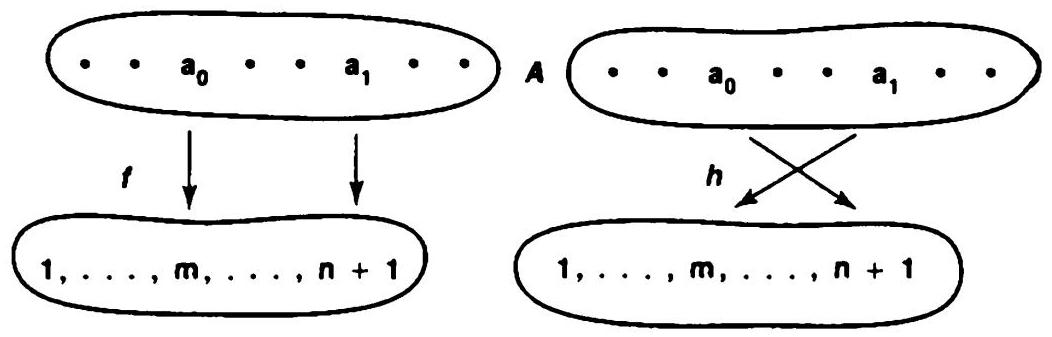
\includegraphics[width=0.9\textwidth]{images/6.1.jpg}
\end{center}
\hspace*{3em} 

Figure 6.1

From this lemma a number of useful con\idx{sequences} follow:
\end{proof}
\begin{theorem} Let \(A\) be a set; suppose that there exists a bijection \(f : A \rightarrow  \{ 1,\ldots ,n\}\) for some \(n \in  {\mathbb{Z}}_{ + }\) . Let \(B\) be a proper subset of \(A\) Then there exists no bijection \(g : B \rightarrow  \{ 1,\ldots ,n\}\) ; but (provided \(B \neq  \varnothing\) ) there does exist a bijection \(h : B \rightarrow  \{ 1,\ldots ,m\}\) for some \(m < n\) .
\end{theorem}

\begin{proof}The case in which \(B = \varnothing\) is trivial, for there cannot exist a bijection of the empty set \(B\) with the nonempty set \(\{ 1,\ldots ,n\}\) .
We prove the theorem ``by induction.'' Let \(C\) be the subset of \({\mathbb{Z}}_{ + }\) consisting of those integers \(n\) for which the theorem holds. We shall show that \(C\) is inductive. From this we conclude that \(C = {\mathbb{Z}}_{ + }\) , so the theorem is true for all positive integers \(n\) .

First we show the theorem is true for \(n = 1\) . In this case \(A\) consists of a single element \(\{ a\}\) , and its only proper subset \(B\) is the empty set.

Now assume that the theorem is true for \(n\) ; we prove it true for \(n + 1\) . Suppose that \(f : A \rightarrow  \{ 1,\ldots ,n + 1\}\) is a bijection, and \(B\) is a nonempty proper subset of \(A\) . Choose an element \({a}_{0}\) of \(B\) and an element \({a}_{1}\) of \(A - B\) . We apply the preceding lemma to conclude there is a bijection

\[
g : A - \left\{  {a}_{0}\right\} \rightarrow  \{ 1,\ldots ,n\} .
\]

Now \(B - \left\{  {a}_{0}\right\}\) is a proper subset of \(A - \left\{  {a}_{0}\right\}\) , for \({a}_{1}\) belongs to \(A - \left\{  {a}_{0}\right\}\) and not to \(B - \left\{  {a}_{0}\right\}\) . Because the theorem has been assumed to hold for the integer \(n\) , we conclude the following

(1) There exists no bijection \(h : B - \left\{  {a}_{0}\right\} \rightarrow  \{ 1,\ldots ,n\}\) .

(2) Either \(B - \left\{  {a}_{0}\right\} = \varnothing\) , or there exists a bijection

\[
k : B - \left\{  {a}_{0}\right\} \rightarrow  \{ 1,\ldots ,p\} \;\text{ for some }p < n.
\]

The preceding lemma, combined with (1), implies that there is no bijection of \(B\) with \(\{ 1,\ldots ,n + 1\}\) . This is the first half of what we wanted to proved. To prove the second half, note that if \(B - \left\{  {a}_{0}\right\} = \varnothing\) , there is a bijection of \(B\) with the set \(\{ 1\}\) ; while if \(B - \left\{  {a}_{0}\right\} \neq  \varnothing\) , we can apply the preceding lemma, along with (2), to conclude that there is a bijection of \(B\) with \(\{ 1,\ldots ,p + 1\}\) . In either case, there is a bijection of \(B\) with \(\{ 1,\ldots ,m\}\) for some \(m < n + 1\) , as desired. The induction principle now shows that the theorem is true for all \(n \in  {\mathbb{Z}}_{ + }\) .
\end{proof}
\begin{corollary} If \(A\) is finite, there is no bijection of \(A\) with a proper subset of itself.
\end{corollary}

\begin{proof}Assume that \(B\) is a proper subset of \(A\) and that \(f : A \rightarrow  B\) is a bijection. By assumption, there is a bijection \(g : A \rightarrow  \{ 1,\ldots ,n\}\) for some \(n\) . The composite \(g \circ  {f}^{-1}\) is then a bijection of \(B\) with \(\{ 1,\ldots ,n\}\) . This contradicts the preceding theorem.\end{proof}
\begin{corollary} \({\mathbb{Z}}_{ + }\) is not finite.
\end{corollary}

\begin{proof}The function \(f : {\mathbb{Z}}_{ + } \rightarrow  {\mathbb{Z}}_{ + } - \{ 1\}\) defined by \(f\left( n\right)  = n + 1\) is a bijection of \({\mathbb{Z}}_{ + }\) with a proper subset of itself.\end{proof}
\begin{corollary} The cardinality of a finite set \(A\) is uniquely determined by \(A\) .
\end{corollary}

\begin{proof}Let \(m < n\) . Suppose there are bijections
\[
f : A \rightarrow  \{ 1,\ldots ,n\}
\]

\[
g : A \rightarrow  \{ 1,\ldots ,m\} \text{ . }
\]

Then the composite

\[
g \circ  {f}^{-1} : \{ 1,\ldots ,n\}  \rightarrow  \{ 1,\ldots ,m\}
\]

is a bijection of the finite set \(\{ 1,\ldots ,n\}\) with a proper subset of itself, contradicting the corollary just proved.
\end{proof}
\begin{corollary} If \(B\) is a subset of the finite set \(A\) , then \(B\) is finite. If \(B\) is a proper subset of \(A\) , then the cardinality of \(B\) is less than the cardinality of \(A\) .
\end{corollary}

\begin{corollary} Let \(B\) be a nonempty set. Then the following are equivalent

(1) \(B\) is finite.

(2) There is a surjective function from a section of the positive integers onto \(B\) .

(3) There is an injective function from \(B\) into a section of the positive integers.
\end{corollary}

\begin{proof}(1) \(\Rightarrow\) (2). Since \(B\) is nonempty, there is, for some \(n\) , a bijective function \(f : \{ 1,\ldots ,n\}  \rightarrow  B\) .
\(\left( 2\right)  \Rightarrow  \left( 3\right)\) . If \(f : \{ 1,\ldots ,n\}  \rightarrow  B\) is surjective, define \(g : B \rightarrow  \{ 1,\ldots ,n\}\) by the equation

\[
g\left( b\right)  = \text{ smallest element of }{f}^{-1}\left( {\{ b\} }\right) .
\]

Because \(f\) is surjective, the set \({f}^{-1}\{ \left( b\right) \}\) is nonempty; then the well-ordering property of \({\mathbb{Z}}_{ + }\) tells us that \(g\left( b\right)\) is uniquely defined. The map \(g\) is injective, for if \(b \neq  {b}^{\prime }\) , then the sets \({f}^{-1}\left( {\{ b\} }\right)\) and \({f}^{-1}\left( \left\{  {b}^{\prime }\right\}  \right)\) are disjoint, so their smallest elements must be different.

\(\left( 3\right)  \Rightarrow  \left( 1\right)\) . If \(g : B \rightarrow  \{ 1,\ldots ,n\}\) is injective, then changing the range of \(g\) gives a bijection of \(B\) with a subset of \(\{ 1,\ldots ,n\}\) . It follows from the preceding corollary that \(B\) is finite.
\end{proof}
\begin{corollary} Finite unions and finite cartesian products of finite sets are finite.
\end{corollary}

\begin{proof}We first show that if \(A\) and \(B\) are finite, so is \(A \cup  B\) . The result is trivial if \(A\) or \(B\) is empty. Otherwise, there are bijections \(f : \{ 1,\ldots ,m\}  \rightarrow  \mathbf{A}\) and \(g\) : \(\{ 1,\ldots ,n\}  \rightarrow  B\) for some choice of \(m\) and \(n\) . Define a function \(h.\{ 1,\ldots ,m +\)  \(n\}  \rightarrow  A \cup  B\) by setting \(h\left( i\right)  = f\left( i\right)\) for \(i = 1,2,\ldots ,m\) and \(h\left( i\right)  = g\left( {i - m}\right)\) for \(i = m + 1,\ldots ,m + n\) . It is easy to check that \(h\) is surjective, from which it follows that \(A \cup  B\) is finite.
Now we show by induction that \idx{Finiteness: of cartesian products} finiteness of the sets \({A}_{1},\ldots ,{A}_{n}\) implies finiteness of their union. This result is trivial for \(n = 1\) Assuming it true for \(n - 1\) , we note that \({A}_{1} \cup  \cdots  \cup  {A}_{n}\) is the union of the two finite sets \({A}_{1} \cup  \cdots  \cup  {A}_{n - 1}\) and \({A}_{n}\) , so the result of the preceding paragraph applies.

Now we show that the cartesian product of two finite sets \(A\) and \(B\) is finite. Given \(a \in  A\) , the set \(\{ a\}  \times  B\) is finite, being in bijective correspondence with \(B\) . The set \(A \times  B\) is the union of these sets; since there are only finitely many of them, \(A \times  B\) is a finite union of finite sets and thus finite.

To prove that the product \({A}_{1} \times  \cdots  \times  {A}_{n}\) is finite if each \({A}_{i}\) is finite, one proceeds by induction.
\end{proof}
\section*{Exercises}

1. (a) Make a list of all the injective maps

\[
f : \{ 1,2,3\}  \rightarrow  \{ 1,2,3,4\} .
\]

Show that none is bijective. (This constitutes a direct proof that a set \(A\) of cardinality three does not have cardinality four.)

(b) How many injective maps

\[
f.\{ 1,\ldots ,8\}  \rightarrow  \{ 1,\ldots ,{10}\}
\]

are there? (You can see why one would not wish to try to prove directly that there is no bijective correspondence between these sets.)

2. Show that if \(B\) is not finite and \(B \subset  A\) , then \(A\) is not finite.

3. Let \(X\) be the two-element set \(\{ 0,1\}\) . Find a bijective correspondence between \({X}^{\omega }\) and a proper subset of itself.

4. Let \(A\) be a nonempty finite simply ordered set.

(a) Show that \(A\) has a largest element. [Hint: Proceed by induction on the cardinality of \(A\) .

(b) Show that \(A\) has the order type of a section of the positive integers.

5. If \(A \times  B\) is finite, does it follow that \(A\) and \(B\) are finite?

6. (a) Let \(A = \{ 1,\ldots ,n\}\) . Show there is a bijection of \(\mathcal{P}\left( A\right)\) with the cartesian product \({X}^{n}\) , where \(X\) is the two-element set \(X = \{ 0,1\}\) .

(b) Show that if \(A\) is finite, then \(\mathcal{P}\left( A\right)\) is finite.

7. If \(A\) and \(B\) are finite, show that the set of all functions \(f : A \rightarrow  B\) is finite.

\section*{§ 7 Countable and Uncountable Sets}

Just as sections of the positive integers are the prototypes for the finite sets, the set of all the positive integers is the prototype for what we call the \idx{countably infinite} sets. In this section, we shall study such sets; we shall also construct some sets that are neither finite nor countably infinite. This study will lead us into a discussion of what we mean by the process of ``inductive definition.''

\begin{definition} A set \(A\) is said to be infinite if it is not finite. It is said to be countably infinite if there is a bijective correspondence

\[
f : A \rightarrow  {\mathbb{Z}}_{ + }\text{ . }
\]
\end{definition}

\begin{example} The set \(\mathbb{Z}\) of all integers is countably infinite. One checks easily that the function \(f : \mathbb{Z} \rightarrow  {\mathbb{Z}}_{ + }\) defined by

\[
f\left( n\right)  = \left\{  \begin{array}{ll} {2n} & \text{ if }n > 0, \\ - {2n} + 1 & \text{ if }n \leq  0 \end{array}\right.
\]

is a bijection.
\end{example}

\begin{example} The product \({\mathbb{Z}}_{ + } \times  {\mathbb{Z}}_{ + }\) is countably infinite. If we represent the elements of the product \({\mathbb{Z}}_{ + } \times  {\mathbb{Z}}_{ + }\) by the integer points in the first quadrant, then the left-hand portion of Figure 7.1 suggests how to ``count'' the points, that is, how to put them in bijective correspondence with the positive integers. A picture is not a proof, of course, but this picture suggests a proof. First, we define a bijection \(f : {\mathbb{Z}}_{ + } \times  {\mathbb{Z}}_{ + } \rightarrow  A\) , where \(A\) is the subset of \({\mathbb{Z}}_{ + } \times  {\mathbb{Z}}_{ + }\) consisting of pairs(x, y)for which \(y \leq  x\) , by the equation

\[
f\left( {x,y}\right)  = \left( {x + y - 1,y}\right) .
\]

Then we construct a bijection of \(A\) with the positive integers, defining \(g : A \rightarrow  {\mathbb{Z}}_{ + }\) by the formula

\[
g\left( {x,y}\right)  = \frac{1}{2}\left( {x - 1}\right) x + y.
\]

We leave it to you to show that \(f\) and \(g\) are bijections.
\end{example}

Another proof that \({\mathbb{Z}}_{ + } \times  {\mathbb{Z}}_{ + }\) is countably infinite will be given later.

\begin{center}
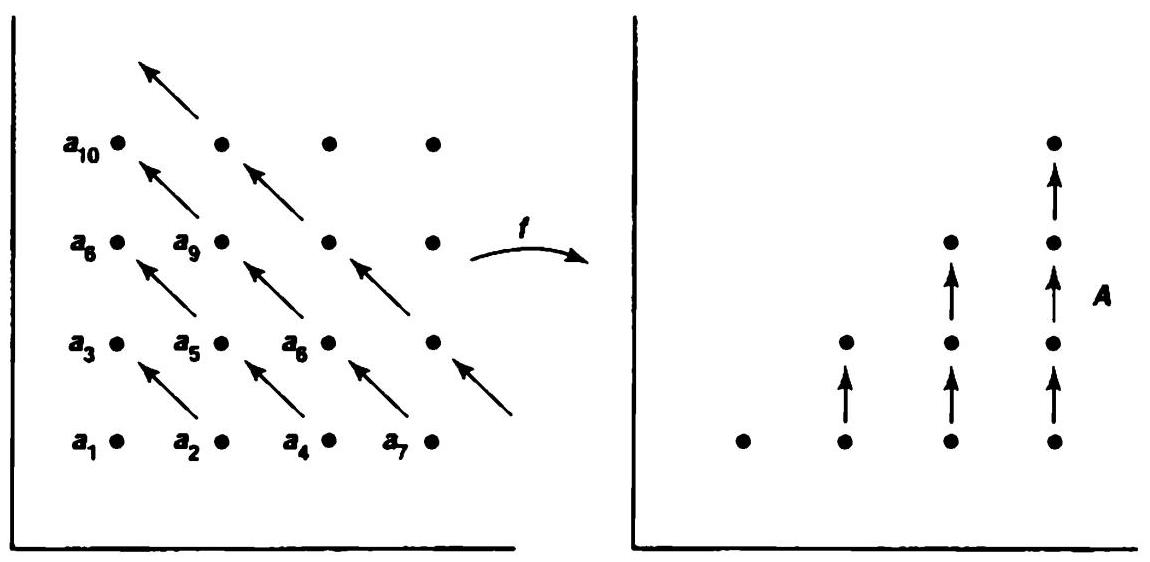
\includegraphics[width=1.0\textwidth]{images/7.1.jpg}
\end{center}
\hspace*{3em} 

Figure 7.1

\begin{definition} A set is said to be countable if it is either finite or countably infinite. A set that is not countable is said to be uncountable.
\end{definition}

There is a very useful criterion for showing that a set is countable. It is the following:

\begin{theorem} Let \(B\) be a nonempty set. Then the following are equivalent:

(1) \(B\) is countable

(2) There is a surjective function \(f : {\mathbb{Z}}_{ + } \rightarrow  B\) .

(3) There is an injective function \(g : B \rightarrow  {\mathbb{Z}}_{ + }\) .

\begin{proof}(1) \(\Rightarrow\) (2). Suppose that \(B\) is countable. If \(B\) is countably infinite, there is a bijection \(f : {\mathbb{Z}}_{ + } \rightarrow  B\) by definition, and we are through. If \(B\) is finite, there is a bijection \(h : \{ 1,\ldots ,n\}  \rightarrow  B\) for some \(n \geq  1\) . (Recall that \(B \neq  \varnothing\) .) We can extend \(h\) to a surjection \(f : {\mathbb{Z}}_{ + } \rightarrow  B\) by defining
\[
f\left( i\right)  = \left\{  \begin{array}{ll} h\left( i\right) & \text{ for }1 \leq  i \leq  n, \\  h\left( 1\right) & \text{ for }i > n. \end{array}\right.
\]

\(\left( 2\right)  \Rightarrow  \left( 3\right)\) . Let \(f : {\mathbb{Z}}_{ + } \rightarrow  B\) be a surjection. Define \(g : B \rightarrow  {\mathbb{Z}}_{ + }\) by the equation

\[
g\left( b\right)  = \text{ smallest element of }{f}^{-1}\left( {\{ b\} }\right) .
\]

Because \(f\) is surjective, \({f}^{-1}\left( {\{ b\} }\right)\) is nonempty; thus \(g\) is well defined. The map \(g\) is injective, for if \(b \neq  {b}^{\prime }\) , the sets \({f}^{-1}\left( {\{ b\} }\right)\) and \({f}^{-1}\left( \left\{  {b}^{\prime }\right\}  \right)\) are disjoint, so their smallest elements are different.

\(\left( 3\right)  \Rightarrow  \left( 1\right)\) . Let \(g : B \rightarrow  {\mathbb{Z}}_{ + }\) be an injection; we wish to prove \(B\) is countable. By changing the range of \(g\) , we can obtain a bijection of \(B\) with a subset of \({\mathbb{Z}}_{ + }\) . Thus to prove our result, it suffices to show that every subset of \({\mathbb{Z}}_{ + }\) is countable. So let \(C\) be a subset of \({\mathbb{Z}}_{ + }\) .

If \(C\) is finite, it is countable by definition. So what we need to prove is that every infinite subset \(C\) of \({\mathbb{Z}}_{ + }\) is countably infinite. This statement is certainly plausible. For the elements of \(C\) can easily be arranged in an infinite sequence; one simply takes the set \({\mathbb{Z}}_{ + }\) in its usual order and ``erases'' all the elements of \({\mathbb{Z}}_{ + }\) that are not in \(C\) !

The plausibility of this argument may make one overlook its informality. Providing a formal proof requires a certain amount of care. We state this result as a separate lemma, which follows.
\end{proof}
\section*{Lemma 7.2. If \(C\) is an infinite subset of \({\mathbb{Z}}_{ + }\) , then \(C\) is countably infinite.}

\begin{proof}We define a bijection \(h : {\mathbb{Z}}_{ + } \rightarrow  C\) . We proceed by induction. Define \(h\left( 1\right)\) to be the smallest element of \(C\) ; it exists because every nonempty subset \(C\) of \({\mathbb{Z}}_{ + }\) has a smallest element. Then assuming that \(h\left( 1\right) ,\ldots ,h\left( {n - 1}\right)\) are defined, define
\[
h\left( n\right)  = \text{ smallest element of }\left\lbrack  {C - h\left( {\{ 1,\ldots ,n - 1\} }\right) }\right\rbrack  .
\]

The set \(C - h\left( {\{ 1,\ldots ,n - 1\} }\right)\) is not empty; for if it were empty, then \(h : \{ 1,\ldots ,n -\)  \(1\}  \rightarrow  C\) would be surjective, so that \(C\) would be finite (by Corollary 6.7). Thus \(h\left( n\right)\) is well defined. By induction, we have defined \(h\left( n\right)\) for all \(n \in  {\mathbb{Z}}_{ + }\) .

To show that \(h\) is injective is easy. Given \(m < n\) , note that \(h\left( m\right)\) belongs to the set \(h\left( {\{ 1,\ldots ,n - 1\} }\right)\) , whereas \(h\left( n\right)\) , by definition, does not. Hence \(h\left( n\right)  \neq  h\left( m\right)\) .

To show that \(h\) is surjective, let \(c\) be any element of \(C\) ; we show that \(c\) lies in the image set of \(h\) . First note that \(h\left( {\mathbb{Z}}_{ + }\right)\) cannot be contained in the finite set \(\{ 1,\ldots ,c\}\) , because \(h\left( {\mathbb{Z}}_{ + }\right)\) is infinite (since \(h\) is injective). Therefore, there is an \(n\) in \({\mathbb{Z}}_{ + }\) , such that \(h\left( n\right)  > c\) . Let \(m\) be the smallest element of \({\mathbb{Z}}_{ + }\) , such that \(h\left( m\right)  \geq  c\) . Then for all \(i < m\) , we must have \(h\left( i\right)  < c\) . Thus, \(c\) does not belong to the set \(h\left( {\{ 1,\ldots ,m - 1\} }\right)\) . Since \(h\left( m\right)\) is defined as the smallest element of the set \(C - h\left( {\{ 1,\ldots ,m - 1\} }\right)\) , we must have \(h\left( m\right)  \leq  c\) . Putting the two inequalities together, we have \(h\left( m\right)  = c\) , as desired.

There is a point in the preceding proof where we stretched the principles of logic a bit. It occurred at the point where we said that ``using the induction principle'' we had defined the function \(h\) for all positive integers \(n\) . You may have seen arguments like this used before, with no questions raised concerning their legitimacy. We have already used such an argument ourselves, in the exercises of \(§4\) , when we defined \({a}^{n}\) .

But there is a problem here. After all, the induction principle states only that if \(A\) is an inductive set of positive integers, then \(A = {\mathbb{Z}}_{ + }\) . To use the principle to prove a theorem ``by induction,'' one begins the proof with the statement ``Let \(A\) be the set of all positive integers \(n\) for which the theorem is true,'' and then one goes ahead to prove that \(A\) is inductive, so that \(A\) must be all of \({\mathbb{Z}}_{ + }\) .

In the preceding theorem, however, we were not really proving a theorem by induction, but defining something by induction. How then should we start the proof? Can we start by saying,''Let \(A\) be the set of all integers \(n\) for which the function \(h\) is defined''? But that’s silly; the symbol \(h\) has no meaning at the outset of the proof. It only takes on meaning in the course of the proof. So something more is needed.

What is needed is another principle, which we call the principle of \idx{Recursive definition, principle} recursive definition. In the proof of the preceding theorem, we wished to assert the following:

Given the infinite subset \(C\) of \({\mathbb{Z}}_{ + }\) , there is a unique function \(h : {\mathbb{Z}}_{ + } \rightarrow  C\) satisfying the formula:

(*)
\[
h\left( 1\right)  = \text{ smallest element of }C\text{ , }
\]

\[
h\left( i\right)  = \text{ smallest element of }\left\lbrack  {C - h\left( {\{ 1,\ldots ,i - 1\} }\right) }\right\rbrack  \;\text{ for all }i > 1\text{ . }
\]

The formula \(\left( *\right)\) is called a recursion formula for \(h\) ; it defines the function \(h\) in terms of itself. A definition given by such a formula is called a recursive definition.

Now one can get into logical difficulties when one tries to define something recursively. Not all recursive formulas make sense. The recursive formula

\[
h\left( i\right)  = \text{ smallest element of }\left\lbrack  {C - h\left( {\{ 1,\ldots ,i + 1\} }\right) }\right\rbrack  .
\]

for example, is self-contradictory; although \(h\left( i\right)\) necessarily is an element of the set \(h\left( {\{ 1,\ldots ,i + 1\} }\right)\) , this formula says that it does not belong to the set. Another example is the classic \idx{Russell's paradox} paradox:

Let the \idx{Barber of Seville paradox} barber of Seville shave every man of Seville who does not shave himself. Who shall shave the barber?

In this statement, the barber appears twice, once in the phrase ``the barber of Seville'' and once as an element of the set ``men of Seville'', this definition of whom the barber shall shave is a recursive one. It also happens to be self-contradictory.

Some recursive formulas do make sense, however Specifically, one has the following principle:

Principle of recursive definition. Let \(A\) be a set. Given a formula that defines \(h\left( 1\right)\) as a unique element of \(A\) , and for \(i > 1\) defines \(h\left( i\right)\) uniquely as an element of \(A\) in terms of the values of \(h\) for positive integers less than \(i\) , this formula determines a unique function \(h : {\mathbb{Z}}_{ + } \rightarrow  A\) .

This principle is the one we actually used in the proof of Lemma 7.2. You can simply accept it on faith if you like. It may however be proved rigorously, using the principle of induction. We shall formulate it more precisely in the next section and indicate how it is proved. Mathematicians seldom refer to this principle specifically. They are much more likely to write a proof like our proof of Lemma 7.2 above, a proof in which they invoke the ``induction principle'' to define a function when what they are really using is the principle of recursive definition. We shall avoid undue pedantry in this book by following their example.
\end{proof}
\begin{corollary} A subset of a countable set is countable.
\end{corollary}

\begin{proof}Suppose \(A \subset  B\) , where \(B\) is countable. There is an injection \(f\) of \(B\) into \({\mathbb{Z}}_{ + }\) ; the restriction of \(f\) to \(A\) is an injection of \(A\) into \({\mathbb{Z}}_{ + }\) .\end{proof}
\begin{corollary} The set \({\mathbb{Z}}_{ + } \times  {\mathbb{Z}}_{ + }\) is countably infinite.
\end{corollary}

\begin{proof}In view of Theorem 7.1, it suffices to construct an injective map \(f : {\mathbb{Z}}_{ + } \times\)  \({\mathbb{Z}}_{ + } \rightarrow  {\mathbb{Z}}_{ + }\) . We define \(f\) by the equation
\[
f\left( {n,m}\right)  = {2}^{n}{3}^{m}.
\]

It is easy to check that \(f\) is injective. For suppose that \({2}^{n}{3}^{m} = {2}^{p}{3}^{q}\) . If \(n < p\) , then \({3}^{m} = {2}^{p - n}{3}^{q}\) , contradicting the fact that \({3}^{m}\) is odd for all \(m\) . Therefore, \(n = p\) . As a result, \({3}^{m} = {3}^{q}\) , Then if \(m < q\) , it follows that \(1 = {3}^{q - m}\) , another contradiction. Hence \(m = q\) .

\begin{example} The set \({\mathbb{Q}}_{ + }\) of positive rational numbers is countably infinite. For we can define a surjection \(g \cdot  {\mathbb{Z}}_{ + } \times  {\mathbb{Z}}_{ + } \rightarrow  {\mathbb{Q}}_{ + }\) by the equation

\[
g\left( {n,m}\right)  = m/n
\]

Because \({\mathbb{Z}}_{ + } \times  {\mathbb{Z}}_{ + }\) is countable, there is a surjection \(f : {\mathbb{Z}}_{ + } \rightarrow  {\mathbb{Z}}_{ + } \times  {\mathbb{Z}}_{ + }\) . Then the composite \(g \circ  f.{\mathbb{Z}}_{ + } \rightarrow  {\mathbb{Q}}_{ + }\) is a surjection, so that \({\mathbb{Q}}_{ + }\) is countable. And, of course, \({\mathbb{Q}}_{ + }\) is infinite because it contains \({\mathbb{Z}}_{ + }\) .
\end{example}

We leave it as an exercise to show the set \(\mathbb{Q}\) of all rational numbers is countably infinite.
\end{proof}
\section*{Theorem 7.5. A countable union of countable sets is countable.}

\begin{proof}Let \({\left\{  {A}_{n}\right\}  }_{n \in  J}\) be an indexed family of countable sets, where the index set \(J\) is either \(\{ 1,\ldots ,N\}\) or \({\mathbb{Z}}_{ + }\) . Assume that each set \({A}_{n}\) is nonempty, for convenience; this assumption does not change anything.
Because each \({A}_{n}\) is countable, we can choose, for each \(n\) , a surjective function \({f}_{n} : {\mathbb{Z}}_{ + } \rightarrow  {A}_{n}\) . Similarly, we can choose a surjective function \(g : {\mathbb{Z}}_{ + } \rightarrow  J\) . Now define

\[
h : {\mathbb{Z}}_{ + } \times  {\mathbb{Z}}_{ + } \rightarrow  \mathop{\bigcup }\limits_{{n \in  J}}{A}_{n}
\]

by the equation

\[
h\left( {k,m}\right)  = {f}_{g\left( k\right) }\left( m\right) .
\]

It is easy to check that \(h\) is surjective. Since \({\mathbb{Z}}_{ + } \times  {\mathbb{Z}}_{ + }\) is in bijective correspondence with \({\mathbb{Z}}_{ + }\) , the \idx{countability} of the union follows from Theorem 7.1.
\end{proof}
\section*{Theorem 7.6. A finite product of countable sets is countable.}

\begin{proof}First let us show that the product of two countable sets \(A\) and \(B\) is countable. The result is trivial if \(A\) or \(B\) is empty. Otherwise, choose surjective functions \(f\) : \({\mathbb{Z}}_{ + } \rightarrow  A\) and \(g : {\mathbb{Z}}_{ + } \rightarrow  B\) . Then the function \(h : {\mathbb{Z}}_{ + } \times  {\mathbb{Z}}_{ + } \rightarrow  A \times  B\) defined by the equation \(h\left( {n,m}\right)  = \left( {f\left( n\right) ,g\left( m\right) }\right)\) is surjective, so that \(A \times  B\) is countable.
In general, we proceed by induction. Assuming that \({A}_{1} \times  \cdots  \times  {A}_{n - 1}\) is countable if each \({A}_{i}\) is countable, we prove the same thing for the product \({A}_{1} \times  \cdots  \times  {A}_{n}\) . First, note that there is a bijective correspondence

\[
g : {A}_{1} \times  \cdots  \times  {A}_{n} \rightarrow  \left( {{A}_{1} \times  \cdots  \times  {A}_{n - 1}}\right)  \times  {A}_{n}
\]

defined by the equation

\[
g\left( {{x}_{1},\ldots ,{x}_{n}}\right)  = \left( {\left( {{x}_{1},\ldots ,{x}_{n - 1}}\right) ,{x}_{n}}\right) .
\]

Because the set \({A}_{1} \times  \cdots  \times  {A}_{n - 1}\) is countable by the induction assumption and \({A}_{n}\) is countable by hypothesis, the product of these two sets is countable, as proved in the preceding paragraph. We conclude that \({A}_{1} \times  \cdots  \times  {A}_{n}\) is countable as well.

It is very tempting to assert that countable products of countable sets should be countable; but this assertion is in fact not true:
\end{proof}
\end{theorem}

\begin{theorem} Let \(X\) denote the two element set \(\{ 0,1\}\) . Then the set \({X}^{\omega }\) is uncountable.
\end{theorem}

\begin{proof}We show that, given any function
\[
g : {\mathbb{Z}}_{ + } \rightarrow  {X}^{\omega }
\]

\(g\) is not surjective. For this purpose, let us denote \(g\left( n\right)\) as follows :

\[
g\left( n\right)  = \left( {{x}_{n1},{x}_{n2},{x}_{n3},\ldots {x}_{nm},\ldots }\right) ,
\]

where each \({x}_{ij}\) is either 0 or 1 . Then we define an element \(\mathbf{y} = \left( {{y}_{1},{y}_{2},\ldots ,{y}_{n},\ldots }\right)\) of \({X}^{\omega }\) by letting

\[
{y}_{n} = \left\{  \begin{array}{ll} 0 & \text{ if }{x}_{nn} = 1, \\  1 & \text{ if }{x}_{nn} = 0. \end{array}\right.
\]

(If we write the numbers \({x}_{n1}\) in a rectangular array, the particular elements \({x}_{nn}\) appear as the diagonal entries in this array; we choose \(\mathbf{y}\) so that its \(n\) th coordinate differs from the diagonal entry \({x}_{nn}\) .)

Now \(\mathbf{y}\) is an element of \({X}^{\omega }\) , and \(\mathbf{y}\) does not lie in the image of \(g\) ; given \(n\) , the point \(g\left( n\right)\) and the point \(y\) differ in at least one coordinate, namely, the \(n\) th. Thus, \(g\) is not surjective.

The cartesian product \(\{ 0,1{\} }^{\omega }\) is one example of an uncountable set. Another is the set \(\mathcal{P}\left( {\mathbb{Z}}_{ + }\right)\) , as the following theorem implies:
\end{proof}
\begin{theorem} Let \(A\) be a set. There is no injective map \(f : \mathcal{P}\left( A\right)  \rightarrow  A\) , and there is no surjective map \(g : A \rightarrow  \mathcal{P}\left( A\right)\) .
\end{theorem}

\begin{proof}In general, if \(B\) is a nonempty set, the existence of an injective map \(f : B \rightarrow\)  \(C\) implies the existence of a surjective map \(g : C \rightarrow  B\) ; one defines \(g\left( c\right)  = {f}^{-1}\left( c\right)\) for each \(c\) in the image set of \(f\) , and defines \(g\) arbitrarily on the rest of \(C\) .
Therefore, it suffices to prove that given a map \(g : A \rightarrow  \mathcal{P}\left( A\right)\) , the map \(g\) is not surjective For each \(a \in  A\) , the image \(g\left( a\right)\) of \(a\) is a subset of \(A\) , which may or may not contain the point \(a\) itself. Let \(B\) be the subset of \(A\) consisting of all those points \(a\) such that \(g\left( a\right)\) does not contain \(a\) ;

\[
B = \{ a \mid  a \in  A - g\left( a\right) \} .
\]

Now, \(B\) may be empty, or it may be all of \(A\) , but that does not matter. We assert that \(B\) is a subset of \(A\) that does not lie in the image of \(g\) . For suppose that \(B = g\left( {a}_{0}\right)\) for some \({a}_{0} \in  A\) . We ask the question: Does \({a}_{0}\) belong to \(B\) or not? By definition of \(B\) ,

\[
{a}_{0} \in  B \Leftrightarrow  {a}_{0} \in  A - g\left( {a}_{0}\right)  \Leftrightarrow  {a}_{0} \in  A - B.
\]

In either case, we have a contradiction.

Now we have proved the existence of uncountable sets. But we have not yet mentioned the most familiar uncountable set of all-the set of real numbers. You have probably seen the uncountability of \(\mathbb{R}\) demonstrated already. If one assumes that every real number can be represented uniquely by an infinite decimal (with the proviso that a representation ending in an infinite string of 9 's is forbidden), then the uncountability of the reals can be proved by a variant of the diagonal procedure used in the proof of Theorem 7.7. But this proof is in some ways not very satisfying. One reason is that the infinite decimal representation of a real number is not at all an elementary consequence of the axioms but requires a good deal of labor to prove. Another reason is that the uncountability of \(\mathbb{R}\) does not, in fact, depend on the infinite decimal expansion of \(\mathbb{R}\) or indeed on any of the algebraic properties of \(\mathbb{R}\) ; it depends on only the order properties of \(\mathbb{R}\) . We shall demonstrate the uncountability of \(\mathbb{R}\) , using only its order properties, in a later chapter.
\end{proof}
\section*{Exercises}

1. Show that \(\mathbb{Q}\) is countably infinite.

2. Show that the maps \(f\) and \(g\) of Examples 1 and 2 are bijections.

3. Let \(X\) be the two-element set \(\{ 0,1\}\) . Show there is a bijective correspondence between the set \(\mathcal{P}\left( {\mathbb{Z}}_{ + }\right)\) and the cartesian product \({X}^{\omega }\) .

4. (a) A real number \(x\) is said to be algebraic (over the rationals) if it satisfies some polynomial equation of positive degree

\[
{x}^{n} + {a}_{n - 1}{x}^{n - 1} + \cdots  + {a}_{1}x + {a}_{0} = 0
\]

with rational coefficients \({a}_{i}\) . Assuming that each polynomial equation has only finitely many roots, show that the set of \idx{algebraic number}s is countable.

(b) A real number is said to be transcendental if it is not algebraic. Assuming the reals are uncountable, show that the \idx{transcendental number}s are uncountable. (It is a somewhat surprising fact that only two transcendental numbers are familiar to us: \(e\) and \(\pi\) . Even proving these two numbers transcendental is highly nontrivial.)

5. Determine, for each of the following sets, whether or not it is countable. Justify your answers.

(a) The set \(A\) of all functions \(f : \{ 0,1\}  \rightarrow  {\mathbb{Z}}_{ + }\) .

(b) The set \({B}_{n}\) of all functions \(f : \{ 1,\ldots ,n\}  \rightarrow  {\mathbb{Z}}_{ + }\) .

(c) The set \(C = \mathop{\bigcup }\limits_{{n \in  {\mathbf{Z}}_{ + }}}{B}_{n}\) .

(d) The set \(D\) of all functions \(f : {\mathbb{Z}}_{ + } \rightarrow  {\mathbb{Z}}_{ + }\) .

(e) The set \(E\) of all functions \(f : {\mathbb{Z}}_{ + } \rightarrow  \{ 0,1\}\) .

(f) The set \(F\) of all functions \(f : {\mathbb{Z}}_{ + } \rightarrow  \{ 0,1\}\) that are ``\idx{eventually zero}.'' [We say that \(f\) is eventually zero if there is a positive integer \(N\) such that \(f\left( n\right)  = 0\) for all \(n \geq  N\) ]

(g) The set \(G\) of all functions \(f : {\mathbb{Z}}_{ + } \rightarrow  {\mathbb{Z}}_{ + }\) that are eventually 1 .

(h) The set \(H\) of all functions \(f : {\mathbb{Z}}_{ + } \rightarrow  {\mathbb{Z}}_{ + }\) that are eventually constant.

(i) The set \(I\) of all two-element subsets of \({\mathbb{Z}}_{ + }\) .

(j) The set \(J\) of all finite subsets of \({\mathbb{Z}}_{ + }\) .

6. We say that two sets \(A\) and \(B\) \idx{have the same cardinality} if there is a bijection of \(A\) with \(B\) .

(a) Show that if \(B \subset  A\) and if there is an injection

\[
f : A \rightarrow  B,
\]

then \(A\) and \(B\) have the same cardinality. [Hint: Define \({A}_{1} = A,{B}_{1} = B\) . and for \(n > 1,{A}_{n} = f\left( {A}_{n - 1}\right)\) and \({B}_{n} = f\left( {B}_{n - 1}\right)\) . (Recursive definition again!) Note that \({A}_{1} \supset  {B}_{1} \supset  {A}_{2} \supset  {B}_{2} \supset  {A}_{3} \supset  \cdots\) . Define a bijection \(h : A \rightarrow  B\) by the rule

\[
h\left( x\right)  = \left\{  \begin{array}{ll} f\left( x\right) & \text{ if }x \in  {A}_{n} - {B}_{n}\text{ for some }n, \\  x & \text{ otherwise.] } \end{array}\right.
\]

(b) Theorem (\idx{Schroeder-Bernstein theorem}). If there are injections \(f : A \rightarrow\)  \(C\) and \(g : C \rightarrow  A\) , then \(A\) and \(C\) have the same cardinality.

7. Show that the sets \(D\) and \(E\) of Exercise 5 have the same cardinality.

8. Let \(X\) denote the two-element set \(\{ 0,1\}\) ; let \(\mathcal{B}\) be the set of countable subsets of \({X}^{\omega }\) . Show that \({X}^{\omega }\) and \(\mathcal{B}\) have the same cardinality.

9. (a) The formula

\[
h\left( 1\right)  = 1,
\]

(*)
\[
h\left( 2\right)  = 2\text{ , }
\]

\[
h\left( n\right)  = {\left\lbrack  h\left( n + 1\right) \right\rbrack  }^{2} - {\left\lbrack  h\left( n - 1\right) \right\rbrack  }^{2}\;\text{ for }n \geq  2
\]

is not one to which the principle of recursive definition applies. Show that nevertheless there does exist a function \(h : {\mathbb{Z}}_{ + } \rightarrow  \mathbb{R}\) satisfying this formula. [Hint: Reformulate (*) so that the principle will apply and require \(h\) to be positive.]

(b) Show that the formula (*) of part (a) does not determine \(h\) uniquely. [Hint: If \(h\) is a positive function satisfying \(\left( *\right)\) , let \(f\left( i\right)  = h\left( i\right)\) for \(i \neq  3\) , and let \(f\left( 3\right)  =  - h\left( 3\right)\) .]

(c) Show that there is no function \(h : {\mathbb{Z}}_{ + } \rightarrow  \mathbb{R}\) satisfying the formula

\[
h\left( 1\right)  = 1,
\]

\[
h\left( 2\right)  = 2,
\]

\[
h\left( n\right)  = {\left\lbrack  h\left( n + 1\right) \right\rbrack  }^{2} + {\left\lbrack  h\left( n - 1\right) \right\rbrack  }^{2}\;\text{ for }n \geq  2.
\]

\section*{*§ 8 The Principle of Recursive Definition}

Before considering the general form of the principle of recursive definition, let us first prove it in a specific case, that of Lemma 7.2. That should make the underlying idea of the proof much clearer when we consider the general case.

So, given the infinite subset \(C\) of \({\mathbb{Z}}_{ + }\) , let us consider the following recursion formula for a function \(h : {\mathbb{Z}}_{ + } \rightarrow  C\) :

(*)
\[
h\left( 1\right)  = \text{ smallest element of }C\text{ , }
\]

\[
h\left( i\right)  = \text{ smallest element of }\left\lbrack  {C - h\left( {\{ 1,\ldots ,i - 1\} }\right) }\right\rbrack  \;\text{ for }i > 1\text{ . }
\]

We shall prove that there exists a unique function \(h : {\mathbb{Z}}_{ + } \rightarrow  C\) satisfying this recursion formula.

The first step is to prove that there exist functions defined on sections \(\{ 1,\ldots ,n\}\) of \({\mathbb{Z}}_{ + }\) that satisfy \(\left( *\right)\) :

\begin{lemma} Given \(n \in  {\mathbb{Z}}_{ + }\) , there exists a function

\[
f : \{ 1,\ldots ,n\}  \rightarrow  C
\]

that satisfies \(\left( *\right)\) for all \(i\) in its domain.
\end{lemma}
\begin{proof} The point of this lemma is that it is a statement that depends on \(n\) ; therefore, it is capable of being proved by induction. Let \(A\) be the set of all \(n\) for which the lemma holds. We show that \(A\) is inductive. It then follows that \(A = {\mathbb{Z}}_{ + }\) .

The lemma is true for \(n = 1\) , since the function \(f : \{ 1\}  \rightarrow  C\) defined by the equation

\[
f\left( 1\right)  = \text{ smallest element of }C
\]

satisfies (*).

Supposing the lemma to be true for \(n - 1\) , we prove it true for \(n\) . By hypothesis, there is a function \({f}^{\prime } : \{ 1,\ldots ,n - 1\}  \rightarrow  C\) satisfying \(\left( *\right)\) for all \(i\) in its domain. Define \(f : \{ 1,\ldots ,n\}  \rightarrow  C\) by the equations

\[
f\left( i\right)  = {f}^{\prime }\left( i\right) \;\text{ for }i \in  \{ 1,\ldots ,n - 1\} ,
\]

\[
f\left( n\right)  = \text{ smallest element of }\left\lbrack  {C - {f}^{\prime }\left( {\{ 1,\ldots ,n - 1\} }\right) }\right\rbrack  .
\]

Since \(C\) is infinite, \({f}^{\prime }\) is not surjective; hence the set \(C - {f}^{\prime }\left( {\{ 1,\ldots ,n - 1\} }\right)\) is not empty, and \(f\left( n\right)\) is well defined. Note that this definition is an acceptable one; it does not define \(f\) in terms of itself but in terms of the given function \({f}^{\prime }\) .

It is easy to check that \(f\) satisfies \(\left( *\right)\) for all \(i\) in its domain. The function \(f\) satisfies \(\left( *\right)\) for \(i \leq  n - 1\) because it equals \({f}^{\prime }\) there. And \(f\) satisfies \(\left( *\right)\) for \(i = n\) because, by definition,

\[
f\left( n\right)  = \text{ smallest element of }\left\lbrack  {C - {f}^{\prime }\left( {\{ 1,\ldots ,n - 1\} }\right) }\right\rbrack
\]

and \({f}^{\prime }\left( {\{ 1,\ldots ,n - 1\} }\right)  = f\left( {\{ 1,\ldots ,n - 1\} }\right)\) .
\end{proof}

\begin{lemma} Suppose that \(f.\{ 1,\ldots ,n\}  \rightarrow  C\) and \(g : \{ 1,\ldots ,m\}  \rightarrow  C\) both satisfy \(\left( *\right)\) for all \(i\) in their respective domains. Then \(f\left( i\right)  = g\left( i\right)\) for all \(i\) in both domains.
\end{lemma}

\begin{proof}Suppose not. Let \(i\) be the smallest integer for which \(f\left( i\right)  \neq  g\left( i\right)\) . The integer \(i\) is not 1, because
\[
f\left( 1\right)  = \text{ smallest element of }C = g\left( 1\right) ,
\]

by \(\left( *\right)\) . Now for all \(j < i\) , we have \(f\left( j\right)  = g\left( j\right)\) . Because \(f\) and \(g\) satisfy \(\left( *\right)\) ,

\[
f\left( i\right)  = \text{ smallest element of }\lbrack C - f\left( {\{ 1,\ldots ,i - 1\} }\right) \} ,
\]

\[
g\left( i\right)  = \text{ smallest element of }\left\lbrack  {C - g\left( {\{ 1,\ldots ,i - 1\} }\right) }\right\rbrack  \text{ . }
\]

Since \(f\left( {\{ 1,\ldots ,i - 1\} }\right)  = g\left( {\{ 1,\ldots ,i - 1\} }\right)\) , we have \(f\left( i\right)  = g\left( i\right)\) , contrary to the choice of \(i\) .
\end{proof}
\begin{theorem} There exists a unique function \(h : {\mathbb{Z}}_{ + } \rightarrow  C\) satisfying \(\left( *\right)\) for all \(i \in  {\mathbb{Z}}_{ + }\) .
\end{theorem}

\begin{proof}By Lemma 8.1, there exists for each \(n\) a function that maps \(\{ 1,\ldots ,n\}\) into \(C\) and satisfies \(\left( *\right)\) for all \(i\) in its domain. Given \(n\) , Lemma 8.2 shows that this function is unique; two such functions having the same domain must be equal. Let \({f}_{n}\) : \(\{ 1,\ldots ,n\}  \rightarrow  C\) denote this unique function.
Now comes the crucial step. We define a function \(h : {\mathbb{Z}}_{ + } \rightarrow  C\) by defining its rule to be the union \(U\) of the rules of the functions \({f}_{n}\) . The rule for \({f}_{n}\) is a subset of \(\{ 1,\ldots ,n\}  \times  C\) ; therefore, \(U\) is a subset of \({\mathbb{Z}}_{ + } \times  C\) . We must show that \(U\) is the rule for a function \(h : {\mathbb{Z}}_{ + } \rightarrow  C\)

That is, we must show that each element \(i\) of \({\mathbb{Z}}_{ + }\) appears as the first coordinate of exactly one element of \(U\) . This is easy. The integer \(i\) lies in the domain of \({f}_{n}\) if and only if \(n > i\) . Therefore, the set of elements of \(U\) of which \(i\) is the first coordinate is precisely the set of all pairs of the form \(\left( {i,{f}_{n}\left( i\right) }\right)\) , for \(n \geq  i\) . Now Lemma 8.2 tells us that \({f}_{n}\left( i\right)  = {f}_{m}\left( i\right)\) if \(n,m \geq  i\) . Therefore, all these elements of \(U\) are equal; that is, there is only one element of \(U\) that has \(i\) as its first coordinate.

To show that \(h\) satisfies \(\left( *\right)\) is also easy; it is a consequence of the following facts:

\[
h\left( i\right)  = {f}_{n}\left( i\right) \;\text{ for }i \leq  n,
\]

\[
{f}_{n}\text{ satisfies }\left( *\right) \text{ for all }i\text{ in its domain. }
\]

The proof of uniqueness is a copy of the proof of Lemma 8.2.

Now we formulate the general principle of recursive definition. There are no new ideas involved in its proof, so we leave it as an exercise.
\end{proof}
\begin{theorem}[Principle of recursive definition] Let \(A\) be a set; let \({a}_{0}\) be an element of \(A\) . Suppose \(\rho\) is a function that assigns, to each function \(f\) mapping a nonempty section of the positive integers into \(A\) , an element of \(A\) . Then there exists a unique function

\[
h : {\mathbb{Z}}_{ + } \rightarrow  A
\]

such that

(*)
\[
h\left( 1\right)  = {a}_{0},
\]

\[
h\left( i\right)  = \rho \left( {h|\{ 1,\ldots ,i - 1\} }\right) \;\text{ for }i > 1.
\]

The formula \(\left( *\right)\) is called a recursion formula for \(h\) . It specifies \(h\left( 1\right)\) , and it expresses the value of \(h\) at \(i > 1\) in terms of the values of \(h\) for positive integers less than \(i\) .

\begin{example} Let us show that Theorem 8.3 is a special case of this theorem. Given the infinite subset \(C\) of \({\mathbb{Z}}_{ + }\) , let \({a}_{0}\) be the smallest element of \(C\) , and define \(\rho\) by the equation

\[
\rho \left( f\right)  = \text{ smallest element of }\left\lbrack  {C - \left( {\text{ image set of }f}\right) }\right\rbrack  \text{ . }
\]

Because \(C\) is infinite and \(f\) is a function mapping a finite set into \(C\) , the image set of \(f\) is not all of \(C\) , therefore, \(\rho\) is well defined. By Theorem 8.4 there exists a function \(h \cdot  {\mathbb{Z}}_{ + } \rightarrow\)  \(C\) such that \(h\left( 1\right)  = {a}_{0}\) , and for \(i > 1\) ,

\[
h\left( i\right)  = \rho \left( {h|\{ 1,\ldots ,i - 1\} }\right)
\]

\[
= \text{ smallest element of }\left\lbrack  {C - \left( {\text{ image set of }h \mid  \{ 1,\ldots ,i - 1\} }\right) }\right\rbrack
\]

\[
= \text{ smallest element of }\left\lbrack  {C - h\left( {\{ 1\ldots ,i - 1\} }\right) }\right\rbrack  \text{ , }
\]

as desired.
\end{example}

\begin{example} Given \(a \in  \mathbb{R}\) , we ``defined'' \({a}^{n}\) , in the exercises of \(\$ 4\) , by the recursion formula

\[
{a}^{1} = a
\]

\[
{a}^{n} = {a}^{n - 1} \cdot  a
\]

We wish to apply Theorem 8.4 to define a function \(h : {\mathbb{Z}}_{ + } \rightarrow  \mathbb{R}\) ngorously such that \(h\left( n\right)  = {a}^{n}\) . To apply this theorem, let \({a}_{0}\) denote the element \(a\) of \(\mathbb{R}\) , and define \(\rho\) by the equation \(\rho \left( f\right)  = f\left( m\right)  \cdot  a\) , where \(f.\{ 1,\ldots ,m\}  \rightarrow  \mathbb{R}\) Then there exists a unique function \(h : {\mathbb{Z}}_{ + } \rightarrow  \mathbb{R}\) such that

\[
h\left( 1\right)  = {a}_{0},
\]

\[
h\left( i\right)  = \rho \left( {h|\{ 1,\ldots ,i - 1\} }\right) \;\text{ for }i > 1.
\]

This means that \(h\left( 1\right)  = a\) , and \(h\left( i\right)  = h\left( {i - 1}\right)  \cdot  a\) for \(i > 1\) . If we denote \(h\left( i\right)\) by \({a}^{i}\) , we have

\[
{a}^{1} = a,
\]

\[
{a}^{l} = {a}^{l - 1} \cdot  a
\]

as desired.
\end{example}

\section*{Exercises}

1. Let \(\left( {{b}_{1},{b}_{2},\ldots }\right)\) be an infinite sequence of real numbers. The sum \(\mathop{\sum }\limits_{{k = 1}}^{n}{b}_{k}\) is defined by induction as follows :

\[
\mathop{\sum }\limits_{{k = 1}}^{n}{b}_{k} = {b}_{1}\;\text{ for }n = 1,
\]

\[
\mathop{\sum }\limits_{{k = 1}}^{n}{b}_{k} = \left( {\mathop{\sum }\limits_{{k = 1}}^{{n - 1}}{b}_{k}}\right)  + {b}_{n}\;\text{ for }n > 1.
\]

Let \(A\) be the set of real numbers; choose \(\rho\) so that Theorem 8.4 applies to define this sum rigorously. We sometimes denote the sum \(\mathop{\sum }\limits_{{k = 1}}^{n}{b}_{k}\) by the symbol \({b}_{1} + {b}_{2} + \cdots  + {b}_{n}\) .

2. Let \(\left( {{b}_{1},{b}_{2},\ldots }\right)\) be an infinite sequence of real numbers. We define the product \(\mathop{\prod }\limits_{{k = 1}}^{n}{b}_{k}\) by the equations

\[
\mathop{\prod }\limits_{{k = 1}}^{1}{b}_{k} = {b}_{1}
\]

\[
\mathop{\prod }\limits_{{k = 1}}^{n}{b}_{k} = \left( {\mathop{\prod }\limits_{{k = 1}}^{{n - 1}}{b}_{k}}\right)  \cdot  {b}_{n}\;\text{ for }n > 1.
\]

Use Theorem 8.4 to define this product rigorously. We sometimes denote the product \(\mathop{\prod }\limits_{{k = 1}}^{n}{b}_{k}\) by the symbol \({b}_{1}{b}_{2}\cdots {b}_{n}\) . 3. Obtain the definitions of \({a}^{n}\) and \(n\) ! for \(n \in  {\mathbb{Z}}_{ + }\) as special cases of Exercise 2. 4. The \idx{Fibonacci numbers} of number theory are defined recursively by the formula

\[
{\lambda }_{1} = {\lambda }_{2} = 1
\]

\[
{\lambda }_{n} = {\lambda }_{n - 1} + {\lambda }_{n - 2}\;\text{ for }n > 2.
\]

Define them rigorously by use of Theorem 8.4.

5. Show that there is a unique function \(h : {\mathbb{Z}}_{ + } \rightarrow  {\mathbb{R}}_{ + }\) satisfying the formula

\[
h\left( 1\right)  = 3,
\]

\[
h\left( i\right)  = {\left\lbrack  h\left( i - 1\right)  + 1\right\rbrack  }^{1/2}\;\text{ for }i > 1.
\]

6. (a) Show that there is no function \(h : {\mathbb{Z}}_{ + } \rightarrow  {\mathbb{R}}_{ + }\) satisfying the formula

\[
h\left( 1\right)  = 3,
\]

\[
h\left( i\right)  = {\left\lbrack  h\left( i - 1\right)  - 1\right\rbrack  }^{1/2}\;\text{ for }i > 1.
\]

Explain why this example does not violate the principle of recursive definition.

(b) Consider the recursion formula

\[
h\left( 1\right)  = 3,
\]

\[
h\left( i\right)  = \left\{  \begin{array}{ll} {\left\lbrack  h\left( i - 1\right)  - 1\right\rbrack  }^{1/2} & \text{ if }h\left( {i - 1}\right)  > 1 \\  5 & \text{ if }h\left( {i - 1}\right)  \leq  1 \end{array}\right\}  \;\text{ for }i > 1.
\]

Show that there exists a unique function \(h : {\mathbb{Z}}_{ + } \rightarrow  {\mathbb{R}}_{ + }\) satisfying this formula.

7. Prove Theorem 8.4.

8. Verify the following version of the principle of recursive definition: Let \(A\) be a set. Let \(\rho\) be a function assigning, to every function \(f\) mapping a section \({S}_{n}\) of \({\mathbb{Z}}_{ + }\) into \(A\) , an element \(\rho \left( f\right)\) of \(A\) . Then there is a unique function \(h : {\mathbb{Z}}_{ + } \rightarrow  A\) such that \(h\left( n\right)  = \rho \left( {h \mid  {S}_{n}}\right)\) for each \(n \in  {\mathbb{Z}}_{ + }\) .

\end{theorem}

\section*{§ 9 Infinite Sets and the Axiom of Choice}

We have already obtained several criteria for a set to be infinite. We know, for instance, that a set \(A\) is infinite if it has a countably infinite subset, or if there is a bijection of \(A\) with a proper subset of itself. It turns out that either of these properties is sufficient to characterize infinite sets. This we shall now prove. The proof will lead us into a discussion of a point of logic we have not yet mentioned-the \idx{axiom of choice}.

\begin{theorem} 
Let \(A\) be a set. The following statements about \(A\) are equivalent:

(1) There exists an injective function \(f : {\mathbb{Z}}_{ + } \rightarrow  A\) .

(2) There exists a bijection of \(A\) with a proper subset of itself.

(3) \(A\) is infinite.
\end{theorem}

\begin{proof}We prove the implications \(\left( 1\right)  \Rightarrow  \left( 2\right)  \Rightarrow  \left( 3\right)  \Rightarrow  \left( 1\right)\) . To prove that \(\left( 1\right)  \Rightarrow  \left( 2\right)\) , we assume there is an injective function \(f : {\mathbb{Z}}_{ + } \rightarrow  A\) . Let the image set \(f\left( {\mathbb{Z}}_{ + }\right)\) be denoted by \(B\) ; and let \(f\left( n\right)\) be denoted by \({a}_{n}\) . Because \(f\) is injective, \({a}_{n} \neq  {a}_{m}\) if \(n \neq  m\) . Define
\[
g : A \rightarrow  A - \left\{  {a}_{1}\right\}
\]

by the equations

\[
g\left( {a}_{n}\right)  = {a}_{n + 1}\;\text{ for }{a}_{n} \in  B.
\]

\[
g\left( x\right)  = x\;\text{ for }x \in  A - B.
\]

The map \(g\) is indicated schematically in Figure 9.1; one checks easily that it is a bijection.

\begin{center}
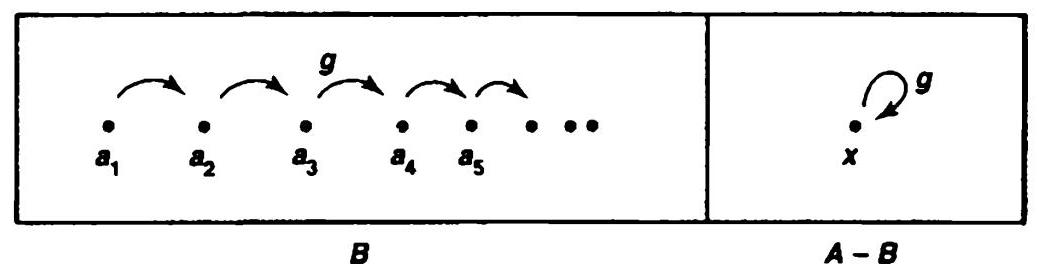
\includegraphics[width=0.9\textwidth]{images/9.1.jpg}
\end{center}
\hspace*{3em} 

Figure 9.1

The implication (2) \(\Rightarrow\) (3) is just the contrapositive of Corollary 6.3, so it has already been proved. To prove that \(\left( 3\right)  \Rightarrow  \left( 1\right)\) , we assume that \(A\) is infinite and construct ``by induction'' an injective function \(f : {\mathbb{Z}}_{ + } \rightarrow  A\) .

First, since the set \(A\) is not empty, we can choose a point \({a}_{1}\) of \(A\) ; define \(f\left( 1\right)\) to be the point so chosen.

Then, assuming that we have defined \(f\left( 1\right) ,\ldots ,f\left( {n - 1}\right)\) , we wish to define \(f\left( n\right)\) . The set \(A - f\left( {\{ 1,\ldots ,n - 1\} }\right)\) is not empty; for if it were empty, the map \(f : \{ 1,\ldots ,n -\)  \(1\}  \rightarrow  A\) would be a surjection and \(A\) would be finite. Hence, we can choose an element of the set \(A - f\left( {\{ 1,\ldots ,n - 1\} }\right)\) and define \(f\left( n\right)\) to be this element. ``Using the induction principle'', we have defined \(f\) for all \(n \in  {\mathbb{Z}}_{ + }\) .

It is easy to see that \(f\) is injective. For suppose that \(m < n\) . Then \(f\left( m\right)\) belongs to the set \(f\left( {\{ 1,\ldots ,n - 1\} }\right)\) , whereas \(f\left( n\right)\) , by definition, does not. Therefore, \(f\left( n\right)  \neq\)  \(f\left( m\right)\) .

Let us try to reformulate this ``induction'' proof more carefully, so as to make explicit our use of the principle of recursive definition.

Given the infinite set \(A\) , we attempt to define \(f : {\mathbb{Z}}_{ + } \rightarrow  A\) recursively by the formula

(*)
\[
f\left( 1\right)  = {a}_{1},
\]

\[
f\left( i\right)  = \text{ an arbitrary element of }\left\lbrack  {A - f\left( {\{ 1,\ldots ,i - 1\} }\right) }\right\rbrack  \;\text{ for }i > 1\text{ . }
\]

But this is not an acceptable recursion formula at all! For it does not define \(f\left( i\right)\) uniquely in terms of \(f \mid  \{ 1,\ldots ,i - 1\}\) .

In this respect this formula differs notably from the recursion formula we considered in proving Lemma 7.2. There we had an infinite subset \(C\) of \({\mathbb{Z}}_{ + }\) , and we defined \(h\) by the formula

\[
h\left( 1\right)  = \text{ smallest element of }C\text{ , }
\]

\[
h\left( i\right)  = \text{ smallest element of }\left\lbrack  {C - h\left( {\{ 1,\ldots ,i - 1\} }\right) }\right\rbrack  \;\text{ for }i > 1\text{ . }
\]

This formula does define \(h\left( i\right)\) uniquely in terms of \(h \mid  \{ 1,\ldots ,i - 1\}\) .

Another way of seeing that \(\left( *\right)\) is not an acceptable recursion formula is to note that if it were, the principle of recursive definition would imply that there is a unique function \(f : {\mathbb{Z}}_{ + } \rightarrow  A\) satisfying \(\left( *\right)\) . But by no stretch of the imagination does \(\left( *\right)\) specify \(f\) uniquely. In fact, this ``definition'' of \(f\) involves infinitely many arbitrary choices.

What we are saying is that the proof we have given for Theorem 9.1 is not actually a proof. Indeed, on the basis of the properties of set theory we have discussed up to now, it is not possible to prove this theorem. Something more is needed.

Previously, we described certain definite allowable methods for specifying sets:

(1) Defining a set by listing its elements, or by taking a given set \(A\) and specifying a subset \(B\) of it by giving a property that the elements of \(B\) are to satisfy.

(2) Taking unions or intersections of the elements of a given collection of sets, or taking the difference of two sets.

(3) Taking the set of all subsets of a given set.

(4) Taking cartesian products of sets.

Now the rule for the function \(f\) is really a set: a subset of \({\mathbb{Z}}_{ + } \times  A\) . Therefore, to prove the existence of the function \(f\) , we must construct the appropriate subset of \({\mathbb{Z}}_{ + } \times  A\) , using the allowed methods for forming sets. The methods already given simply are not adequate for this purpose. We need a new way of asserting the existence of a set. So, we add to the list of allowed methods of forming sets the following: Axiom of choice. Given a collection \(\mathcal{A}\) of disjoint nonempty sets, there exists a set \(C\) consisting of exactly one element from each element of \(\mathcal{A}\) ; that is, a set \(\mathbf{C}\) such that \(\mathbf{C}\) is contained in the union of the elements of \(\mathcal{A}\) , and for each \(A \in  \mathcal{A}\) , the set \(C \cap  A\) contains a single element.

The set \(C\) can be thought of as having been obtained by choosing one element from each of the sets in \(\mathcal{A}\) .

The axiom of choice certainly seems an innocent-enough assertion. And, in fact, most mathematicians today accept it as part of the set theory on which they base their mathematics. But in years past a good deal of controversy raged around this particular assertion concerning set theory, for there are theorems one can prove with its aid that some mathematicians were reluctant to accept. One such is the \idx{well-ordering theorem}, which we shall discuss shortly. For the present we shall simply use the choice axiom to clear up the difficulty we mentioned in the preceding proof. First, we prove an easy consequence of the axiom of choice:
\end{proof}
\begin{lemma}[Existence of a \idx{choice function}] Given a collection \(\mathcal{B}\) of nonempty sets (not necessarily disjoint), there exists a function

\[
c : \mathcal{B} \rightarrow  \mathop{\bigcup }\limits_{{B \in  \mathcal{B}}}B
\]

such that \(c\left( B\right)\) is an element of \(B\) , for each \(B \in  \mathcal{B}\) .

The function \(c\) is called a choice function for the collection \(\mathcal{B}\) .

The difference between this lemma and the axiom of choice is that in this lemma the sets of the collection \(\mathcal{B}\) are not required to be disjoint. For example, one can allow \(\mathcal{B}\) to be the collection of all nonempty subsets of a given set.
\end{lemma}

Proof of the lemma. Given an element \(B\) of \(\mathcal{B}\) , we define a set \({B}^{\prime }\) as follows

\[
{B}^{\prime } = \{ \left( {B,x}\right)  \mid  x \in  B\} .
\]

That is, \({B}^{\prime }\) is the collection of all ordered pairs, where the first coordinate of the ordered pair is the set \(B\) , and the second coordinate is an element of \(B\) . The set \({B}^{\prime }\) is a subset of the cartesian product

\[
\mathcal{B} \times  \mathop{\bigcup }\limits_{{B \in  \mathcal{B}}}B
\]

Because \(B\) contains at least one element \(x\) , the set \({B}^{\prime }\) contains at least the element (B, x), so it is nonempty.

Now we claim that if \({B}_{1}\) and \({B}_{2}\) are two different sets in \(\mathcal{B}\) , then the corresponding sets \({B}_{1}^{\prime }\) and \({B}_{2}^{\prime }\) are disjoint. For the typical element of \({B}_{1}^{\prime }\) is a pair of the form \(\left( {{B}_{1},{x}_{1}}\right)\) and the typical element of \({B}_{2}^{\prime }\) is a pair of the form \(\left( {{B}_{2},{x}_{2}}\right)\) . No two such elements can be equal, for their first coordinates are different. Now let us form the collection

\[
C = \left\{  {{B}^{\prime } \mid  B \in  \mathcal{B}}\right\}  \text{ ; }
\]

it is a collection of disjoint nonempty subsets of

\[
\mathcal{B} \times  \mathop{\bigcup }\limits_{{B \in  \mathcal{B}}}B
\]

By the choice axiom, there exists a set \(c\) consisting of exactly one element from each element of \(\mathcal{C}\) . Our claim is that \(c\) is the rule for the desired choice function.

In the first place, \(c\) is a subset of

\[
\mathcal{B} \times  \mathop{\bigcup }\limits_{{B \in  \mathcal{B}}}B
\]

In the second place, \(c\) contains exactly one element from each set \({B}^{\prime }\) ; therefore, for each \(B \in  \mathcal{B}\) , the set \(c\) contains exactly one ordered pair(B, x)whose first coordinate is \(B\) . Thus \(c\) is indeed the rule for a function from the collection \(\mathcal{B}\) to the set \(\mathop{\bigcup }\limits_{{B \in  \mathcal{B}}}B\) . Finally, if \(\left( {B,x}\right)  \in  c\) , then \(x\) belongs to \(B\) , so that \(c\left( B\right)  \in  B\) , as desired.

A second proof of Theorem 9.1. Using this lemma, one can make the proof of Theorem 9.1 more precise. Given the infinite set \(A\) , we wish to construct an injective function \(f : {\mathbb{Z}}_{ + } \rightarrow  A\) . Let us form the collection \(\mathcal{B}\) of all nonempty subsets of \(A\) . The lemma just proved asserts the existence of a choice function for \(\mathcal{B}\) ; that is, a function

\[
c : \mathcal{B} \rightarrow  \mathop{\bigcup }\limits_{{B \in  \mathcal{B}}}B = A
\]

such that \(c\left( B\right)  \in  B\) for each \(B \in  \mathcal{B}\) . Let us now define a function \(f : {\mathbb{Z}}_{ + } \rightarrow  A\) by the recursion formula

(*)
\[
f\left( 1\right)  = c\left( A\right)
\]

\[
f\left( i\right)  = c\left( {A - f\left( {\{ 1,\ldots ,i - 1\} }\right) }\right) \;\text{ for }i > 1.
\]

Because \(A\) is infinite, the set \(A - f\left( {\{ 1,\ldots ,i - 1\} }\right)\) is nonempty; therefore, the right side of this equation makes sense. Since this formula defines \(f\left( i\right)\) uniquely in terms of \(f \mid  \{ 1,\ldots ,i - 1\}\) , the principle of recursive definition applies. We conclude that there exists a unique function \(f : {\mathbb{Z}}_{ + } \rightarrow  A\) satisfying \(\left( *\right)\) for all \(i \in  {\mathbb{Z}}_{ + }\) . Injectivity of \(f\) follows as before.

Having emphasized that in order to construct a proof of Theorem 9.1 that is logically correct, one must make specific use of a choice function, we now backtrack and admit that in practice most mathematicians do no such thing. They go on with no qualms giving proofs like our first version, proofs that involve an infinite number of arbitrary choices. They know that they are really using the choice axiom; and they know that if it were necessary, they could put their proofs into a logically more satisfactory form by introducing a choice function specifically. But usually they do not bother.

And neither will we. You will find few further specific uses of a choice function in this book; we shall introduce a choice function only when the proof would become confusing without it. But there will be many proofs in which we make an infinite number of arbitrary choices, and in each such case we will actually be using the choice axiom implicitly.

Now we must confess that in an earlier section of this book there is a proof in which we constructed a certain function by making an infinite number of arbitrary choices. And we slipped that proof in without even mentioning the choice axiom. Our apologies for the deception. We leave it to you to ferret out which proof it was!

Let us make one final comment on the choice axiom. There are two forms of this axiom. One can be called the \idx{finite axiom of choice}; it asserts that given a finite collection \(\mathcal{A}\) of disjoint nonempty sets, there exists a set \(C\) consisting of exactly one element from each element of \(\mathcal{A}\) . One needs this weak form of the choice axiom all the time; we have used it freely in the preceding sections with no comment. No mathematician has any qualms about the finite choice axiom; it is part of everyone's set theory. Said differently, no one has qualms about a proof that involves only finitely many arbitrary choices.

The stronger form of the axiom of choice, the one that applies to an arbitrary collection \(\mathcal{A}\) of nonempty sets, is the one that is properly called ``the axiom of choice.'' When a mathematician writes, ``This proof depends on the choice axiom,'' it is invariably this stronger form of the axiom that is meant.

\section*{Exercises}

1. Define an injective map \(f : {\mathbb{Z}}_{ + } \rightarrow  {X}^{\omega }\) , where \(X\) is the two-element set \(\{ 0,1\}\) , without using the choice axiom.

2. Find if possible a choice function for each of the following collections, without using the choice axiom:

(a) The collection \(\mathcal{A}\) of nonempty subsets of \({\mathbb{Z}}_{ + }\) .

(b) The collection \(\mathcal{B}\) of nonempty subsets of \(\mathbb{Z}\) .

(c) The collection \(\mathcal{C}\) of nonempty subsets of the rational numbers \(\mathbb{Q}\) .

(d) The collection \(\mathcal{D}\) of nonempty subsets of \({X}^{\omega }\) , where \(X = \{ 0,1\}\) .

3. Suppose that \(A\) is a set and \({\left\{  {f}_{n}\right\}  }_{n \in  {\mathbf{Z}}_{ + }}\) is a given indexed family of injective functions

\[
{f}_{n} : \{ 1,\ldots ,n\}  \rightarrow  A
\]

Show that \(A\) is infinite. Can you define an injective function \(f : {\mathbb{Z}}_{ + } \rightarrow  A\) without using the choice axiom?

4. There was a theorem in \(§7\) whose proof involved an infinite number of arbitrary choices. Which one was it? Rewrite the proof so as to make explicit the use of the choice axiom. (Several of the earlier exercises have used the choice axiom also.)

5. (a) Use the choice axiom to show that if \(f : A \rightarrow  B\) is surjective, then \(f\) has a right inverse \(h \cdot  B \rightarrow  A\) .

(b) Show that if \(f : A \rightarrow  B\) is injective and \(A\) is not empty, then \(f\) has a left inverse. Is the axiom of choice needed?

6. Most of the famous paradoxes of naive set theory are associated in some way or other with the concept of the ``set of all sets.'' None of the rules we have given for forming sets allows us to consider such a set. And for good reason-the concept itself is self-contradictory. For suppose that \(\mathcal{A}\) denotes the ``set of all sets.''

(a) Show that \(\mathcal{P}\left( \mathcal{A}\right)  \subset  \mathcal{A}\) ; derive a contradiction.

(b) (Russell’s paradox.) Let \(\mathcal{B}\) be the subset of \(\mathcal{A}\) consisting of all sets that are not elements of themselves;

\[
\mathcal{B} = \{ A \mid  A \in  \mathcal{A}\text{ and }A \notin  A\} .
\]

(Of course, there may be no set \(A\) such that \(A \in  A\) ; if such is the case, then \(\mathcal{B} = \mathcal{A}\) .) Is \(\mathcal{B}\) an element of itself or not?

7. Let \(A\) and \(B\) be two nonempty sets. If there is an injection of \(B\) into \(A\) , but no injection of \(A\) into \(B\) , we say that \(A\) has \idx{greater cardinality} than \(B\) .

(a) Conclude from Theorem 9.1 that every uncountable set has greater cardinality than \({\mathbb{Z}}_{ + }\) .

(b) Show that if \(A\) has greater cardinality than \(B\) , and \(B\) has greater cardinality than \(C\) , then \(A\) has greater cardinality than \(C\) .

(c) Find a sequence \({A}_{1},{A}_{2},\ldots\) of infinite sets, such that for each \(n \in  {\mathbb{Z}}_{ + }\) , the set \({A}_{n + 1}\) has greater cardinality than \({A}_{n}\) .

(d) Find a set that for every \(n\) has cardinality greater than \({A}_{n}\) .

*8. Show that \(\mathcal{P}\left( {\mathbb{Z}}_{ + }\right)\) and \(\mathbb{R}\) have the same cardinality. [Hint: You may use the fact that every real number has a decimal expansion, which is unique if expansions that end in an infinite string of 9 ’s are forbidden.]

A famous conjecture of set theory, called the \idx{continuum hypothesis}, asserts that there exists no set having greater cardinality than \({\mathbb{Z}}_{ + }\) and lesser cardinality than \(\mathbb{R}\) . The \idx{generalized continuum hypothesis} asserts that, given the infinite set \(A\) , there is no set having greater cardinality than \(A\) and lesser cardinality than \(\mathcal{P}\left( A\right)\) . Surprisingly enough, both of these assertions have been shown to be independent of the usual axioms for set theory. For a readable expository account, see \cite{Smullyan1969}.

\section*{§ 10 Well-Ordered Sets}

One of the useful properties of the set \({\mathbb{Z}}_{ + }\) of positive integers is the fact that each of its nonempty subsets has a smallest element. Generalizing this property leads to the concept of a \idx{well-ordered set}.

\begin{definition} A set \(A\) with an order relation \(<\) is said to be well-ordered if every nonempty subset of \(A\) has a smallest element.
\end{definition}

\begin{example} Consider the set \(\{ 1,2\}  \times  {\mathbb{Z}}_{ + }\) in the dictionary ordering. Schernatically, it can be represented as one infinite sequence followed by another infinite sequence:

\[
{a}_{1},{a}_{2},{a}_{3},\ldots ;{b}_{1},{b}_{2},{b}_{3},\ldots
\]

with the understanding that each element is less than every element to the right of it. It is not difficult to see that every nonempty subset \(C\) of this ordered set has a smallest element: If \(C\) contains any one of the elements \({a}_{n}\) , we simply take the smallest element of the intersection of \(C\) with the sequence \({a}_{1},{a}_{2},\ldots\) ; while if \(C\) contains no \({a}_{n}\) , then it is a subset of the sequence \({b}_{1},{b}_{2},\ldots\) and as such has a smallest element.
\end{example}

\begin{example} Consider the set \({\mathbb{Z}}_{ + } \times  {\mathbb{Z}}_{ + }\) in the dictionary order. Schematically, it can be represented as an infinite sequence of infinite sequences. We show that it is well-ordered. Let \(X\) be a nonempty subset of \({\mathbb{Z}}_{ + } \times  {\mathbb{Z}}_{ + }\) Let \(A\) be the subset of \({\mathbb{Z}}_{ + }\) consisting of all first coordinates of elements of \(X\) Now \(A\) has a smallest element; call it \({a}_{0}\) . Then the collection

\[
\left\{  {b \mid  {a}_{0} \times  b \in  X}\right\}
\]

is a nonempty subset of \({\mathbb{Z}}_{ + }\) ; let \({b}_{0}\) be its smallest element. By definition of the dictionary order, \({a}_{0} \times  {b}_{0}\) is the smallest element of \(X\) . See Figure 10.1.

\begin{center}
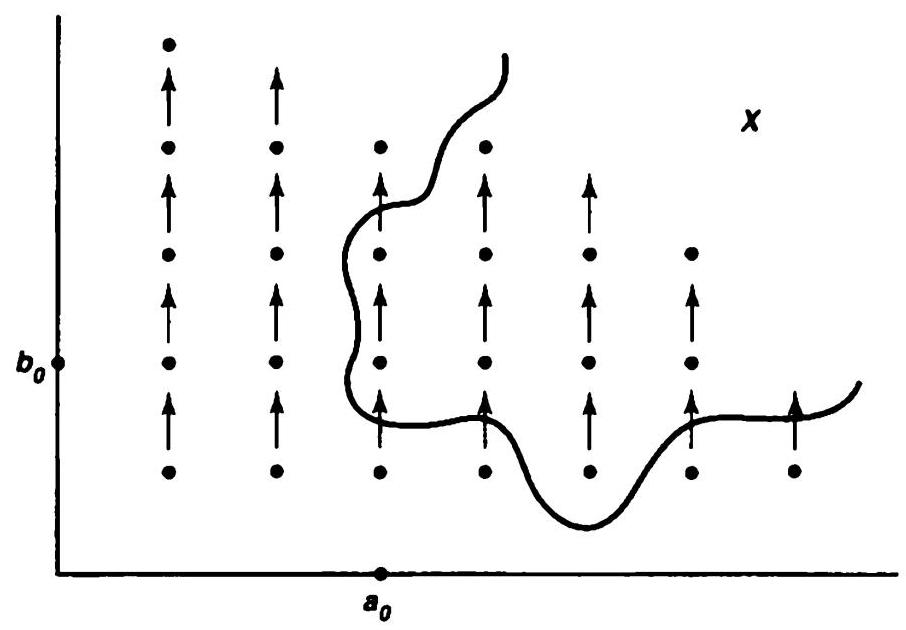
\includegraphics[width=0.8\textwidth]{images/10.1.jpg}
\end{center}
\hspace*{3em} 

Figure 10.1
\end{example}

\begin{example} The set of integers is not well-ordered in the usual order, the subset consisting of the negative integers has no smallest element. Nor is the set of real numbers in the interval \(0 \leq  x \leq  1\) well-ordered; the subset consisting of those \(x\) for which \(0 < x < 1\) has no smallest element (although it has a greatest lower bound, of course).
\end{example}

There are several ways of constructing well-ordered sets. Two of them are the following:

(1) If \(A\) is a well-ordered set, then any subset of \(A\) is well-ordered in the restricted order relation.

(2) If \(A\) and \(B\) are well-ordered sets, then \(A \times  B\) is well-ordered in the dictionary order.

The proof of (1) is trivial; the proof of (2) follows the pattern given in Example 2.

It follows that the set \({\mathbb{Z}}_{ + } \times  \left( {{\mathbb{Z}}_{ + } \times  {\mathbb{Z}}_{ + }}\right)\) is well-ordered in the dictionary order; it can be represented as an infinite sequence of infinite sequences of infinite sequences. Similarly, \({\left( {\mathbb{Z}}_{ + }\right) }^{4}\) is well-ordered in the dictionary order. And so on. But if you try to generalize to an infinite product of \({\mathbb{Z}}_{ + }\) with itself, you will run into trouble. We shall examine this situation shortly.

Now, given a set \(A\) without an order relation, it is natural to ask whether there exists an order relation for \(A\) that makes it into a well-ordered set. If \(A\) is finite, any bijection

\[
f : A \rightarrow  \{ 1,\ldots ,n\}
\]

can be used to define an order relation on \(A\) ; under this relation, \(A\) has the same order type as the ordered set \(\{ 1,\ldots ,n\}\) . In fact, every order relation on a finite set can be obtained in this way:

\begin{theorem} Every nonempty finite ordered set has the order type of a section \(\{ 1,\ldots ,n\}\) of \({\mathbb{Z}}_{ + }\) , so it is well-ordered.
\end{theorem}

\begin{proof}This was given as an exercise in \(\$ 6\) ; we prove it here. First, we show that every finite ordered set \(A\) has a largest element. If \(A\) has one element, this is trivial. Supposing it true for sets having \(n - 1\) elements, let \(A\) have \(n\) elements and let \({a}_{0} \in  A\) . Then \(A - \left\{  {a}_{0}\right\}\) has a largest element \({a}_{1}\) , and the larger of \(\left\{  {{a}_{0},{a}_{1}}\right\}\) is the largest element of \(A\) .
Second, we show there is an order-preserving bijection of \(A\) with \(\{ 1,\ldots ,n\}\) for some \(n\) . If \(A\) has one element, this fact is trivial. Suppose that it is true for sets having \(n - 1\) elements. Let \(b\) be the largest element of \(A\) . By hypothesis, there is an order-preserving bijection

\[
{f}^{\prime } : A - \{ b\}  \rightarrow  \{ 1,\ldots ,n - 1\} .
\]

Define an order-preserving bijection \(f : A \rightarrow  \{ 1,\ldots ,n\}\) by setting

\[
f\left( x\right)  = {f}^{\prime }\left( x\right) \;\text{ for }x \neq  b,
\]

\[
f\left( b\right)  = n\text{ . }
\]

Thus, a finite ordered set has only one possible order type. For an infinite set, things are quite different. The well-ordered sets

\[
{\mathbb{Z}}_{ + }\text{ , }
\]

\[
\{ 1,\ldots ,n\}  \times  {\mathbb{Z}}_{ + },
\]

\[
{\mathbb{Z}}_{ + } \times  {\mathbb{Z}}_{ + }
\]

\[
{\mathbb{Z}}_{ + } \times  \left( {{\mathbb{Z}}_{ + } \times  {\mathbb{Z}}_{ + }}\right)
\]

are all countably infinite, but they all have different order types, as you can check.

All the examples we have given of well-ordered sets are orderings of countable sets. It is natural to ask whether one can find a well-ordered uncountable set.

The obvious uncountable set to try is the countably infinite product

\[
X = {\mathbb{Z}}_{ + } \times  {\mathbb{Z}}_{ + } \times  \cdots  = {\left( {\mathbb{Z}}_{ + }\right) }^{\omega }
\]

of \({\mathbb{Z}}_{ + }\) with itself. One can generalize the dictionary order to this set in a natural way, by defining

\[
\left( {{a}_{1},{a}_{2},\ldots }\right)  < \left( {{b}_{1},{b}_{2},\ldots }\right)
\]

if for some \(n \geq  1\) ,

\[
{a}_{i} = {b}_{i},\;\text{ for }i < n\text{ and }{a}_{n} < {b}_{n}.
\]

This is, in fact, an order relation on the set \(X\) ; but unfortunately it is not a well-ordering. Consider the set \(A\) of all elements \(\mathbf{x}\) of \(X\) of the form

\[
\mathbf{x} = \left( {1,\ldots ,1,2,1,1,\ldots }\right) ,
\]

where exactly one coordinate of \(\mathbf{x}\) equals 2, and the others are all equal to 1 . The set \(A\) clearly has no smallest element.

Thus, the dictionary order at least does not give a well-ordering of the set \({\left( {\mathbb{Z}}_{ + }\right) }^{\omega }\) . Is there some other order relation on this set that is a well-ordering? No one has ever constructed a specific well-ordering of \({\left( {\mathbb{Z}}_{ + }\right) }^{\omega }\) . Nevertheless, there is a famous theorem that says such a well-ordering exists:
\end{proof}
\begin{theorem}[Well-ordering theorem] If \(A\) is a set, there exists an order relation on \(A\) that is a well-ordering.
\end{theorem}

This theorem was proved by \idx{Zermelo} in 1904, and it startled the mathematical world. There was considerable debate as to the correctness of the proof; the lack of any constructive procedure for well-ordering an arbitrary uncountable set led many to be skeptical. When the proof was analyzed closely, the only point at which it was found that there might be some question was a construction involving an infinite number of arbitrary choices, that is, a construction involving-the choice axiom.

Some mathematicians rejected the choice axiom as a result, and for many years a legitimate question about a new theorem was: Does its proof involve the choice axiom or not? A theorem was considered to be on somewhat shaky ground if one had to use the choice axiom in its proof. Present-day mathematicians, by and large, do not have such qualms. They accept the axiom of choice as a reasonable assumption about set theory, and they accept the well-ordering theorem along with it.

The proof that the choice axiom implies the well-ordering theorem is rather long (although not exceedingly difficult) and primarily of interest to logicians, we shall omit it. If you are interested, a proof is outlined in the supplementary exercises at the end of the chapter. Instead, we shall simply assume the well-ordering theorem whenever we need it. Consider it to be an additional axiom of set theory if you like!

We shall in fact need the full strength of this assumption only occasionally. Most of the time, all we need is the following weaker result:

\section*{Corollary. There exists an uncountable well-ordered set.}

We now use this result to construct a particular well-ordered set that will prove to be very useful.

\begin{definition} Let \(X\) be a well-ordered set Given \(\alpha  \in  X\) , let \(\idxmath{S}{\({S}_{\alpha }\) (section of well-ordered set)} {S}_{\alpha }\) denote the set

\[
{S}_{\alpha } = \{ x \mid  x \in  X\text{ and }x < \alpha \} .
\]

It is called the section of \(X\) by \(\alpha\) .
\end{definition}

\begin{lemma} There exists a well-ordered set \(A\) having a largest element \(\Omega\) , such that the section \(\idxmath{S}{\({S}_{\Omega }\)} {S}_{\Omega }\) of \(A\) by \(\Omega\) is uncountable but every other section of \(A\) is countable.
\end{lemma}

\begin{proof}We begin with an uncountable well-ordered set \(B\) Let \(C\) be the well-ordered set \(\{ 1,2\}  \times  B\) in the dictionary order; then some section of \(C\) is uncountable. (Indeed, the section of \(C\) by any element of the form \(2 \times  b\) is uncountable.) Let \(\Omega\) be the smallest element of \(C\) for which the section of \(C\) by \(\Omega\) is uncountable Then let \(A\) consist of this section along with the element \(\Omega\) .
Note that \({S}_{\Omega }\) is an uncountable well-ordered set every section of which is countable Its order type is in fact uniquely determined by this condition. We shall call it a minimal uncountable well-ordered set. Furthermore, we shall denote the well-ordered set \(A = {S}_{\Omega } \cup  \{ \Omega \}\) by the symbol \({\widetilde{S}}_{\Omega }\) (for reasons to be seen later)

The most useful property of the set \({S}_{\Omega }\) for our purposes is expressed in the following theorem
\end{proof}
\begin{theorem} If \(A\) is a countable subset of \({S}_{\Omega }\) , then \(A\) has an upper bound in \({S}_{\Omega }\) .
\end{theorem}

\begin{proof}Let \(A\) be a countable subset of \({S}_{\Omega }\) . For each \(a \in  A\) , the section \({S}_{a}\) is countable. Therefore, the union \(B = \mathop{\bigcup }\limits_{{a \in  A}}{S}_{a}\) is also countable Since \({S}_{\Omega }\) is uncountable, the set \(B\) is not all of \({S}_{\Omega }\) ; let \(x\) be a point of \({S}_{\Omega }\) that is not in \(B\) . Then \(x\) is an upper bound for \(A\) . For if \(x < a\) for some \(a\) in \(A\) , then \(x\) belongs to \({S}_{a}\) and hence to \(B\) , contrary to choice.\end{proof}
\section*{Exercises}

1. Show that every well-ordered set has the least upper bound property.

2. (a) Show that in a well-ordered set, every element except the largest (if one exists) has an immediate successor.

(b) Find a set in which every element has an immediate successor that is not well-ordered.

3. Both \(\{ 1,2\}  \times  {\mathbb{Z}}_{ + }\) and \({\mathbb{Z}}_{ + } \times  \{ 1,2\}\) are well-ordered in the dictionary order. Do they have the same order type?

4. (a) Let \({\mathbb{Z}}_{ - }\) denote the set of negative integers in the usual order. Show that a simply ordered set \(A\) fails to be well-ordered if and only if it contains a subset having the same order type as \({\mathbb{Z}}_{ - }\) .

(b) Show that if \(A\) is simply ordered and every countable subset of \(A\) is well-ordered, then \(A\) is well-ordered.

5. Show the well-ordering theorem implies the choice axiom.

6. Let \({S}_{\Omega }\) be the minimal uncountable well-ordered set.

(a) Show that \({S}_{\Omega }\) has no largest element.

(b) Show that for every \(\alpha  \in  {S}_{\Omega }\) , the subset \(\{ x \mid  \alpha  < x\}\) is uncountable.

(c) Let \({X}_{0}\) be the subset of \({S}_{\Omega }\) consisting of all elements \(x\) such that \(x\) has no immediate predecessor. Show that \({X}_{0}\) is uncountable.

7. Let \(J\) be a well-ordered set. A subset \({J}_{0}\) of \(J\) is said to be inductive if for every \(\alpha  \in  J,\)

\[
\left( {{S}_{\alpha } \subset  {J}_{0}}\right)  \Rightarrow  \alpha  \in  {J}_{0}
\]

\begin{theorem}[The principle of \idx{transfinite induction}] If \(J\) is a well-ordered set and \({J}_{0}\) is an inductive subset of \(J\) , then \({J}_{0} = J\) .
\end{theorem}

8. (a) Let \({A}_{1}\) and \({A}_{2}\) be \idx{disjoint sets}, well-ordered by \({ < }_{1}\) and \({ < }_{2}\) , respectively. Define an order relation on \({A}_{1} \cup  {A}_{2}\) by letting \(a < b\) either if \(a,b \in  {A}_{1}\) and \(a{ < }_{1}b\) , or if \(a,b \in  {A}_{2}\) and \(a{ < }_{2}b\) , or if \(a \in  {A}_{1}\) and \(b \in  {A}_{2}\) . Show that this is a well-ordering

(b) Generalize (a) to an arbitrary family of disjoint well-ordered sets, indexed by a well-ordered set.

9. Consider the subset \(A\) of \({\left( {\mathbb{Z}}_{ + }\right) }^{\omega }\) consisting of all infinite sequences of positive integers \(\mathbf{x} = \left( {{x}_{1},{x}_{2},\ldots }\right)\) that end in an infinite string of 1 ’s. Give \(A\) the following order: \(\mathbf{x} < \mathbf{y}\) if \({x}_{n} < {y}_{n}\) and \({x}_{i} = {y}_{i}\) for \(i > n\) . We call this the ``antidictionary order'' on \(A\) .

(a) Show that for every \(n\) , there is a section of \(A\) that has the same order type as \({\left( {\mathbb{Z}}_{ + }\right) }^{n}\) in the dictionary order.

(b) Show \(A\) is well-ordered.

10. Theorem. Let \(J\) and \(C\) be well-ordered sets; assume that there is no surjective function mapping a section of \(J\) onto \(C\) . Then there exists a unique function \(h : J \rightarrow  C\) satisfying the equation

(*)
\[
h\left( x\right)  = \text{ smallest }\left\lbrack  {C - h\left( {S}_{x}\right) }\right\rbrack
\]

for each \(x \in  J\) , where \({S}_{x}\) is the section of \(J\) by \(x\) .

Proof

(a) If \(h\) and \(k\) map sections of \(J\) , or all of \(J\) , into \(C\) and satisfy (*) for all \(x\) in their respective domains, show that \(h\left( x\right)  = k\left( x\right)\) for all \(x\) in both domains.

(b) If there exists a function \(h : {S}_{\alpha } \rightarrow  C\) satisfying \(\left( *\right)\) , show that there exists a function \(k \cdot  {S}_{\alpha } \cup  \{ \alpha \}  \rightarrow  C\) satisfying \(\left( *\right)\) .

(c) If \(K \subset  J\) and for all \(\alpha  \in  K\) there exists a function \({h}_{\alpha } \cdot  {S}_{\alpha } \rightarrow  C\) satisfying \(\left( *\right)\) , show that there exists a function

\[
k : \mathop{\bigcup }\limits_{{\alpha  \in  K}}{S}_{\alpha } \rightarrow  C
\]

satisfying \(\left( *\right)\) .

(d) Show by transfinite induction that for every \(\beta  \in  J\) , there exists a function \({h}_{\beta } : {S}_{\beta } \rightarrow  C\) satisfying \(\left( *\right)\) . [Hint: If \(\beta\) has an immediate predecessor \(\alpha\) , then \({S}_{\beta } = {S}_{\alpha } \cup  \{ \alpha \}\) . If not, \({S}_{\beta }\) is the union of all \({S}_{\alpha }\) with \(\alpha  < \beta\) .]

(e) Prove the theorem.

11. Let \(A\) and \(B\) be two sets Using the well-ordering theorem, prove that either they have the same cardinality, or one has cardinality greater than the other. [Hint: If there is no surjection \(f : A \rightarrow  B\) , apply the preceding exercise.]

\section*{*§ 11 The Maximum Principle \protect\sectionDagger}

We have already indicated that the axiom of choice leads to the deep theorem that every set can be well-ordered. The axiom of choice has other consequences that are even more important in mathematics. Collectively referred to as ``\idx{maximum principle}s,'' they come in many versions Formulated independently by a number of mathematicians, including F. Hausdorff, K. Kuratowski, S. Bochner, and M. Zorn, during the years 1914-1935, they were typically proved as consequences of the well-ordering theorem. Later, it was realized that they were in fact equivalent to the well-ordering theorem. We consider several of them here.

First, we make a definition. Given a set \(A\) , a relation \(\prec\) on \(A\) is called a strict partial order on \(A\) if it has the following two properties:

(1) (Nonreflexivity) The relation \(a \prec  a\) never holds.

(2) (Transitivity) If \(a \prec  b\) and \(b \prec  c\) , then \(a \prec  c\) .

These are just the second and third of the properties of a simple order (see §3); the comparability property is the one that is omitted. In other words, a strict partial order behaves just like a simple order except that it need not be true that for every pair of distinct points \(x\) and \(y\) in the set, either \(x \prec  y\) or \(y \prec  x\) .

If \(\prec\) is a strict partial order on a set \(A\) , it can easily happen that some subset \(B\) of \(A\) is simply ordered by the relation; all that is needed is for every pair of elements of \(B\) to be comparable under \(\prec\) .

\customfootnote{${}^{\dagger}$ This section will be assumed in Chapters 5 and 14.}



Now we can state the following principle, which was first formulated by Hausdorff in 1914.

\begin{theorem}[The maximum principle] Let \(A\) be a set; let \(\prec\) be a strict partial order on \(A\) . Then there exists a maximal simply ordered subset \(B\) of \(A\) .
\end{theorem}

Said differently, there exists a subset \(B\) of \(A\) such that \(B\) is simply ordered by \(\prec\) and such that no subset of \(A\) that properly contains \(B\) is simply ordered by \(\prec\) .

\begin{example} If \(\mathcal{A}\) is any collection of sets, the relation ``is a proper subset of'' is a strict partial order on \(\mathcal{A}\) . Suppose that \(\mathcal{A}\) is the collection of all circular regions (interiors of circles) in the plane. One maximal simply ordered subcollection of \(\mathcal{A}\) consists of all circular regions with centers at the origin Another maximal simply ordered subcollection consists of all circular regions bounded by circles tangent from the right to the \(y\) -axis at the origin See Figure 11 1.

\begin{center}
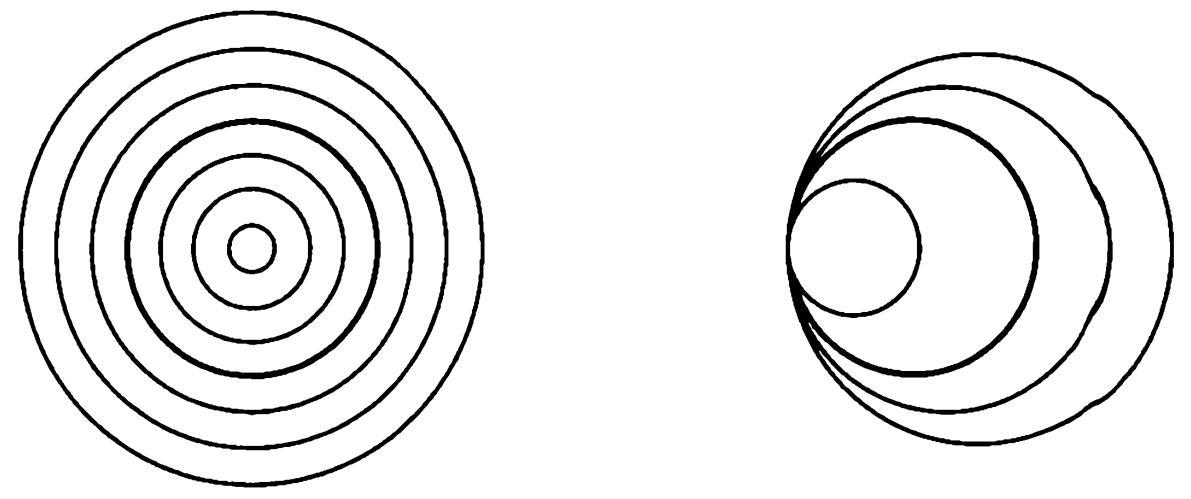
\includegraphics[width=1.0\textwidth]{images/11.1.jpg}
\end{center}
\hspace*{3em}

Figure 11.1
\end{example}

\begin{example} If \(\left( {{x}_{0},{y}_{0}}\right)\) and \(\left( {{x}_{1},{y}_{1}}\right)\) are two points of the plane \({\mathbb{R}}^{2}\) , define

\[
\left( {{x}_{0},{y}_{0}}\right)  \prec  \left( {{x}_{1},{y}_{1}}\right)
\]

If \({y}_{0} = {y}_{1}\) and \({x}_{0} < {x}_{1}\) This is a partial ordering of \({\mathbb{R}}^{2}\) under which two points are comparable only if they lie on the same horizontal line The maximal simply ordered sets are the horizontal lines in \({\mathbb{R}}^{2}\)
\end{example}

One can give an intuitive ``proof'' of the maximum principle that is rather appealing. It involves a step-by-step procedure, which one can describe in physical terms as follows. Suppose we take a box, and put into it some of the elements of \(A\) according to the following plan: First we pick an arbitrary element of \(A\) and put it in the box. Then we pick another element of \(A\) . If it is comparable with the element in the box, we put it in the box too; otherwise, we throw it away. At the general step, we will have a collection of elements in the box and a collection of elements that have been tossed away. Take one of the remaining elements of \(A\) If it is comparable with everything in the box, toss it in the box, too, otherwise, throw it away. Similarly continue. After you have checked all the elements of \(A\) , the elements you have in the box will be comparable with one another, and thus they will form a simply ordered set. Every element not in the box will be noncomparable with at least one element in the box, for that was why it was tossed away. Hence, the simply ordered set in the box is maximal, for no larger subset of \(A\) can satisfy the comparability condution

Now of course the weak point in the preceding ``proof'' comes when we said, ``After you have checked all the elements of \(A\) .'' How do you know you ever ``get through'' checking all the elements of \(A\) ? If \(A\) should happen to be countable, it is not hard to make this intuitive proof into a real proof. Let us take the countably infinite case; the finite case is even easier. Index the elements of \(A\) bijectively with the positive integers, so that \(A = \left\{  {{a}_{1},{a}_{2}\ldots }\right\}\) . This indexing gives a way of deciding what order to test the elements of \(A\) in, and how to know when one has tested them all.

Now we define a function \(h : {\mathbb{Z}}_{ + } \rightarrow  \{ 0,1\}\) , by letting it assign the value 0 to \(i\) if we ``put \({a}_{i}\) in the box,'' and the value 1 if we ``throw \({a}_{i}\) away.'' This means that \(h\left( 1\right)  = 0\) , and for \(i > 1\) , we have \(h\left( i\right)  = 0\) if and only if \({a}_{i}\) is comparable with every element of the set

\[
\left\{  {{a}_{j} \mid  j < i\text{ and }h\left( j\right)  = 0}\right\}  \text{ . }
\]

By the principle of recursive definition, this formula determines a unique function \(h.{\mathbb{Z}}_{ + } \rightarrow  \{ 0,1\}\) It is easy to check that the set of those \({a}_{j}\) for which \(h\left( j\right)  = 0\) is a maximal simply ordered subset of \(A\) .

If \(A\) is not countable, a variant of this procedure will work, if we allow ourselves to use the well-ordering theorem. Instead of indexing the elements of \(A\) with the set \({\mathbb{Z}}_{ + }\) , we index them (in a bijective fashion) with the elements of some well-ordered set \(J\) , so that \(A = \left\{  {{a}_{\alpha } \mid  \alpha  \in  J}\right\}\) . For this we need the well-ordering theorem, so that we know there is a bijection between \(A\) and some well-ordered set \(J\) . Then we can proceed as in the previous paragraph, letting \(\alpha\) replace \(i\) in the argument. Strictly speaking, you need to generalize the principle of recursive definition to well-ordered sets as well, but that is not particularly difficult. (See the Supplementary Exercises.)

Thus, the well-ordering theorem implies the maximum principle.

Although the maximum principle of Hausdorff was the first to be formulated and is probably the simplest to understand, there is another such principle that is nowadays the one most frequently quoted. It is popularly called ``\idx{Zorn's Lemma},'' although Ku-ratowski (1922) and Bochner (1922) preceded Zorn (1935) in enunciating and proving versions of it. For a history and discussion of the tangled history of these ideas, see \cite{Campbell1978} or \cite{Moore1982}. To state this principle, we need some terminology.

\begin{definition} Let \(A\) be a set and let \(\prec\) be a strict partial order on \(A\) . If \(B\) is a subset of \(A\) , an upper bound on \(B\) is an element \(c\) of \(A\) such that for every \(b\) in \(B\) , either \(b = c\) or \(b \prec  c\) . A \idx{maximal element} of \(A\) is an element \(m\) of \(A\) such that for no element \(a\) of \(A\) does the relation \(m \prec  a\) hold.
\end{definition}

Zorn's Lemma. Let \(A\) be a set that is strictly partially ordered. If every simply ordered subset of \(A\) has an upper bound in \(A\) , then \(A\) has a maximal element.

Zorn’s lemma is an easy consequence of the maximum principle: Given \(A\) , the maximum principle implies that \(A\) has a maximal simply ordered subset \(B\) . The hypothesis of Zorn’s lemma tells us that \(B\) has an upper bound \(c\) in \(A\) . The element \(c\) is then automatically a maximal element of \(A\) . For if \(c \prec  d\) for some element \(d\) of \(A\) , then the set \(B \cup  \{ d\}\) , which properly contains \(B\) , is simply ordered because \(b \prec  d\) for every \(b \in  B\) . This fact contradicts maximality of \(B\) .

It is also true that the maximum principle is an easy consequence of Zorn's lemma. See Exercises 5-7.

One final remark. We have defined what we mean by a strict partial order on a set, but we have not said what a partial order itself is. Let \(\prec\) be a strict partial order on a set \(A\) Suppose that we define \(a \preccurlyeq  b\) if either \(a \prec  b\) or \(a = b\) . Then the relation \(\preccurlyeq\) is called a partial order on \(A\) For example, the inclusion relation \(\subset\) on a collection of sets is a partial order, whereas proper inclusion is a strict partial order.

Many authors prefer to deal with partial orderings rather than strict partial orderings, the maximum principle and Zorn's lemma are often expressed in these terms. Which formulation is used is simply a matter of taste and convenience.

\section*{Exercises}

1. If \(a\) and \(b\) are real numbers, define \(a \prec  b\) if \(b - a\) is positive and rational. Show this is a strict partial order on \(\mathbb{R}\) . What are the maximal simply ordered subsets?

2. (a) Let \(\prec\) be a strict partial order on the set \(A\) . Define a relation on \(A\) by letting \(a \preccurlyeq  b\) if either \(a \prec  b\) or \(a = b\) . Show that this relation has the following properties, which are called the partial order axioms:

(i) \(a \preccurlyeq  a\) for all \(a \in  A\) .

(ii) \(a \preccurlyeq  b\) and \(b \preccurlyeq  a \Rightarrow  a = b\) .

(iii) \(a \preccurlyeq  b\) and \(b \preccurlyeq  c \Rightarrow  a \preccurlyeq  c\) .

(b) Let \(P\) be a relation on \(A\) that satisfies properties (i)-(iii). Define a relation \(S\) on \(A\) by letting \({aSb}\) if \({aPb}\) and \(a \neq  b\) . Show that \(S\) is a strict partial order on \(A\) .

3. Let \(A\) be a set with a strict partial order \(\prec\) ; let \(x \in  A\) . Suppose that we wish to find a maximal simply ordered subset \(B\) of \(A\) that contains \(x\) . One plausible way of attempting to define \(B\) is to let \(B\) equal the set of all those elements of \(A\) that are comparable with \(x\) ;

\[
B = \{ y \mid  y \in  A\text{ and either }x \prec  y\text{ or }y \prec  x\} .
\]

But this will not always work. In which of Examples 1 and 2 will this procedure succeed and in which will it not?

4. Given two points \(\left( {{x}_{0},{y}_{0}}\right)\) and \(\left( {{x}_{1},{y}_{1}}\right)\) of \({\mathbb{R}}^{2}\) , define

\[
\left( {{x}_{0},{y}_{0}}\right)  \prec  \left( {{x}_{1},{y}_{1}}\right)
\]

if \({x}_{0} < {x}_{1}\) and \({y}_{0} \leq  {y}_{1}\) . Show that the curves \(y = {x}^{3}\) and \(y = 2\) are maximal simply ordered subsets of \({\mathbb{R}}^{2}\) , and the curve \(y = {x}^{2}\) is not. Find all maximal simply ordered subsets.

5. Show that Zorn's lemma implies the following:

\begin{lemma}[Kuratowski] Let \(\mathcal{A}\) be a collection of sets. Suppose that for every subcollection \(\mathcal{B}\) of \(\mathcal{A}\) that is simply ordered by proper inclusion, the union of the elements of \(\mathcal{B}\) belongs to \(\mathcal{A}\) Then \(\mathcal{A}\) has an element that is properly contained in no other element of \(\mathcal{A}\) .
\end{lemma}

6. A collection \(\mathcal{A}\) of subsets of a set \(X\) is said to be of finite type provided that a subset \(B\) of \(X\) belongs to \(\mathcal{A}\) if and only if every finite subset of \(B\) belongs to \(\mathcal{A}\) . Show that the \idx{Kuratowski lemma} implies the following.

\begin{lemma}[Tukey, 1940] Let \(\mathcal{A}\) be a collection of sets. If \(\mathcal{A}\) is of finite type, then \(\mathcal{A}\) has an element that is properly contained in no other element of \(\mathcal{A}\) .
\end{lemma}

7. Show that the \idx{Tukey lemma} implies the \idx{Hausdorff maximum principle}. [Hint: If \(\prec\) is a strict partial order on \(A\) , let \(\mathcal{A}\) be the collection of all subsets of \(A\) that are simply ordered by \(\prec\) . Show that \(\mathcal{A}\) is of finite type.)

8. A typical use of Zorn's lemma in algebra is the proof that every vector space has a basis. Recall that if \(A\) is a subset of the vector space \(V\) , we say a vector belongs to the span of \(A\) if it equals a finite linear combination of elements of \(A\) . The set \(A\) is independent if the only finite linear combination of elements of \(A\) that equals the zero vector is the trivial one having all coefficients zero. If \(A\) is independent and if every vector in \(V\) belongs to the span of \(A\) , then \(A\) is a basis for \(V\) .

(a) If \(A\) is independent and \(v \in  V\) does not belong to the span of \(A\) , show \(A \cup  \{ v\}\) is independent.

(b) Show the collection of all independent sets in \(V\) has a maximal element.

(c) Show that \(V\) has a basis.

\section*{* Supplementary Exercises: Well-Ordering}

In the following exercises, we ask you to prove the equivalence of the choice axiom, the well-ordering theorem, and the maximum principle. We comment that of these exercises, only Exercise 7 uses the choice axiom.

1. Theorem (General principle of recursive definition). Let \(J\) be a well-ordered set; let \(C\) be a set. Let \(\mathcal{F}\) be the set of all functions mapping sections of \(J\) into \(C\) . Given a function \(\rho  : \mathcal{F} \rightarrow  C\) , there exists a unique function \(h : J \rightarrow  C\) such that \(h\left( \alpha \right)  = \rho \left( {h \mid  {S}_{\alpha }}\right)\) for each \(\alpha  \in  J\) .

[Hint: Follow the pattern outlined in Exercise 10 of \(§{10}\) .]

2. (a) Let \(J\) and \(E\) be well-ordered sets, let \(h : J \rightarrow  E\) . Show the following two statements are equivalent:

(i) \(h\) is order preserving and its image is \(E\) or a section of \(E\) .

(ii) \(h\left( \alpha \right)  =\) smallest \(\left\lbrack  {E - h\left( {S}_{\alpha }\right) }\right\rbrack\) for all \(\alpha\) .

[Hint: Show that each of these conditions implies that \(h\left( {S}_{\alpha }\right)\) is a section of \(E\) , conclude that it must be the section by \(h\left( \alpha \right)\) .]

(b) If \(E\) is a well-ordered set, show that no section of \(E\) has the order type of \(E\) , nor do two different sections of \(E\) have the same order type. [Hint: Given \(J\) , there is at most one order-preserving map of \(J\) into \(E\) whose image is \(E\) or a section of \(E\) .]

3. Let \(J\) and \(E\) be well-ordered sets; suppose there is an order-preserving map \(k : J \rightarrow  E\) . Using Exercises 1 and 2, show that \(J\) has the order type of \(E\) or a section of \(E\) . [Hint: Choose \({e}_{0} \in  E\) . Define \(h : J \rightarrow  E\) by the recursion formula

\[
h\left( \alpha \right)  = \text{ smallest }\left\lbrack  {E - h\left( {S}_{\alpha }\right) }\right\rbrack  \;\text{ if }\;h\left( {S}_{\alpha }\right)  \neq  E,
\]

and \(h\left( \alpha \right)  = {e}_{0}\) otherwise. Show that \(h\left( \alpha \right)  \leq  k\left( \alpha \right)\) for all \(\alpha\) ; conclude that \(\left. {h\left( {S}_{\alpha }\right)  \neq  E\text{ for all }\alpha .}\right\rbrack\)

4. Use Exercises 1-3 to prove the following

(a) If \(A\) and \(B\) are well-ordered sets, then exactly one of the following three conditions holds: \(A\) and \(B\) have the same order type, or \(A\) has the order type of a section of \(B\) , or \(B\) has the order type of a section of \(A\) . [Hint: Form a well-ordered set containing both \(A\) and \(B\) , as in Exercise 8 of \(§{10}\) ; then apply the preceding exercise.]

(b) Suppose that \(A\) and \(B\) are well-ordered sets that are uncountable, such that every section of \(A\) and of \(B\) is countable. Show \(A\) and \(B\) have the same order type.

5. Let \(X\) be a set; let \(\mathcal{A}\) be the collection of all pairs \(\left( {A, < }\right)\) , where \(A\) is a subset of \(X\) and \(<\) is a well-ordering of \(A\) . Define

\[
\left( {A, < }\right)  \prec  \left( {{A}^{\prime },{ < }^{\prime }}\right)
\]

if \(\left( {A, < }\right)\) equals a section of \(\left( {{A}^{\prime },{ < }^{\prime }}\right)\) .

(a) Show that \(\prec\) is a strict partial order on \(\mathcal{A}\) .

(b) Let \(\mathcal{B}\) be a subcollection of \(\mathcal{A}\) that is simply ordered by \(\prec\) . Define \({B}^{\prime }\) to be the union of the sets \(B\) , for all \(\left( {B, < }\right)  \in  \mathcal{B}\) ; and define \({ < }^{\prime }\) to be the union of the relations \(<\) , for all \(\left( {B, < }\right)  \in  \mathcal{B}\) . Show that \(\left( {{B}^{\prime },{ < }^{\prime }}\right)\) is a well-ordered set.

6. Use Exercises 1 and 5 to prove the following:

\begin{theorem} The maximum principle is equivalent to the well-ordering theorem.
\end{theorem}

7. Use Exercises 1-5 to prove the following.

\begin{theorem} The choice axiom is equivalent to the well-ordering theorem.
\end{theorem}
\begin{proof} Let \(X\) be a set, let \(c\) be a fixed choice function for the nonempty subsets of \(X\) . If \(T\) is a subset of \(X\) and \(<\) is a relation on \(T\) , we say that \(\left( {T, < }\right)\) is a tower in \(X\) if \(<\) is a well-ordering of \(T\) and if for each \(x \in  T\) ,

\[
x = c\left( {X - {S}_{x}\left( T\right) }\right) ,
\]

where \({S}_{x}\left( T\right)\) is the section of \(T\) by \(x\) .

(a) Let \(\left( {{T}_{1},{ < }_{1}}\right)\) and \(\left( {{T}_{2},{ < }_{2}}\right)\) be two towers in \(X\) . Show that either these two ordered sets are the same, or one equals a section of the other. [Hint: Switching indices if necessary, we can assume that \(h : {T}_{1} \rightarrow  {T}_{2}\) is order preserving and \(h\left( {T}_{1}\right)\) equals either \({T}_{2}\) or a section of \({T}_{2}\) . Use Exercise 2 to show that \(h\left( x\right)  = x\) for all \(x\) .]

(b) If \(\left( {T, < }\right)\) is a tower in \(X\) and \(T \neq  X\) , show there is a tower in \(X\) of which \(\left( {T, < }\right)\) is a section.

(c) Let \(\left\{  {\left( {{T}_{k},{ < }_{k}}\right)  \mid  k \in  K}\right\}\) be the collection of all towers in \(X\) . Let

\[
T = \mathop{\bigcup }\limits_{{k \in  K}}{T}_{k}\;\text{ and }\; <  = \mathop{\bigcup }\limits_{{k \in  K}}\left( { < }_{k}\right) .
\]

Show that \(\left( {T, < }\right)\) is a tower in \(X\) . Conclude that \(T = X\) .

8. Using Exercises 1-4, construct an uncountable well-ordered set, as follows. Let \(A\) be the collection of all pairs \(\left( {A, < }\right)\) , where \(A\) is a subset of \({\mathbb{Z}}_{ + }\) and \(<\) is a well-ordering of \(A\) . (We allow \(A\) to be empty.) Define \(\left( {A, < }\right)  \sim  \left( {{A}^{\prime },{ < }^{\prime }}\right)\) if \(\left( {A, < }\right)\) and \(\left( {{A}^{\prime },{ < }^{\prime }}\right)\) have the same order type. It is trivial to show this is an equivalence relation. Let \(\left\lbrack  \left( {A, < }\right) \right\rbrack\) denote the equivalence class of \(\left( {A, < }\right)\) ; let \(E\) denote the collection of these equivalence classes. Define

\[
\left\lbrack  \left( {A, < }\right) \right\rbrack \ll  \left\lbrack  \left( {{A}^{\prime },{ < }^{\prime }}\right) \right\rbrack
\]

if \(\left( {A, < }\right)\) has the order type of a section of \(\left( {{A}^{\prime },{ < }^{\prime }}\right)\) .

(a) Show that the relation \(\ll\) is well defined and is a simple order on \(E\) . Note that the equivalence class \(\left\lbrack  \left( {\varnothing ,\varnothing }\right) \right\rbrack\) is the smallest element of \(E\) .

(b) Show that if \(\alpha  = \left\lbrack  \left( {A, < }\right) \right\rbrack\) is an element of \(E\) , then \(\left( {A, < }\right)\) has the same order type as the section \({S}_{\alpha }\left( E\right)\) of \(E\) by \(\alpha\) . [Hint: Define a map \(f : A \rightarrow  E\) by setting \(f\left( x\right)  = \left\lbrack  \left( {{S}_{x}\left( A\right) \text{ , restriction of } < }\right) \right\rbrack\) for each \(x \in  A\) .]

(c) Conclude that \(E\) is well-ordered by \(\ll\) .

(d) Show that \(E\) is uncountable. [Hint: If \(h : E \rightarrow  {\mathbb{Z}}_{ + }\) is a bijection, then \(h\) gives rise to a well-ordering of \({\mathbb{Z}}_{ + }\) .]
\end{proof}

This same argument, with \({\mathbb{Z}}_{ + }\) replaced by an arbitrary well-ordered set \(X\) , proves (without use of the choice axiom) the existence of a well-ordered set \(E\) whose cardinality is greater than that of \(X\) .

This exercise shows that one can construct an uncountable well-ordered set, and hence the minimal uncountable well-ordered set, by an explicit construction that does not use the choice axiom. However, this result is less interesting than it might appear. The crucial property of \({S}_{\Omega }\) , the one we use repeatedly, is the fact that every countable subset of \({S}_{\Omega }\) has an upper bound in \({S}_{\Omega }\) . That fact depends, in turn, on the fact that a countable union of countable sets is countable. And the proof of that result (if you examine it carefully) involves an infinite number of arbitrary choices-that is, it depends on the choice axiom.

Said differently, without the choice axiom we may be able to construct the minimal uncountable well-ordered set, but we can't use it for anything!